\documentclass[twoside]{book}

% Packages required by doxygen
\usepackage{calc}
\usepackage{doxygen}
\usepackage{graphicx}
\usepackage[utf8]{inputenc}
\usepackage{makeidx}
\usepackage{multicol}
\usepackage{multirow}
\usepackage{textcomp}
\usepackage[table]{xcolor}

% Font selection
\usepackage[T1]{fontenc}
\usepackage{mathptmx}
\usepackage[scaled=.90]{helvet}
\usepackage{courier}
\usepackage{amssymb}
\usepackage{sectsty}
\renewcommand{\familydefault}{\sfdefault}
\allsectionsfont{%
  \fontseries{bc}\selectfont%
  \color{darkgray}%
}
\renewcommand{\DoxyLabelFont}{%
  \fontseries{bc}\selectfont%
  \color{darkgray}%
}

% Page & text layout
\usepackage{geometry}
\geometry{%
  a4paper,%
  top=2.5cm,%
  bottom=2.5cm,%
  left=2.5cm,%
  right=2.5cm%
}
\tolerance=750
\hfuzz=15pt
\hbadness=750
\setlength{\emergencystretch}{15pt}
\setlength{\parindent}{0cm}
\setlength{\parskip}{0.2cm}
\makeatletter
\renewcommand{\paragraph}{%
  \@startsection{paragraph}{4}{0ex}{-1.0ex}{1.0ex}{%
    \normalfont\normalsize\bfseries\SS@parafont%
  }%
}
\renewcommand{\subparagraph}{%
  \@startsection{subparagraph}{5}{0ex}{-1.0ex}{1.0ex}{%
    \normalfont\normalsize\bfseries\SS@subparafont%
  }%
}
\makeatother

% Headers & footers
\usepackage{fancyhdr}
\pagestyle{fancyplain}
\fancyhead[LE]{\fancyplain{}{\bfseries\thepage}}
\fancyhead[CE]{\fancyplain{}{}}
\fancyhead[RE]{\fancyplain{}{\bfseries\leftmark}}
\fancyhead[LO]{\fancyplain{}{\bfseries\rightmark}}
\fancyhead[CO]{\fancyplain{}{}}
\fancyhead[RO]{\fancyplain{}{\bfseries\thepage}}
\fancyfoot[LE]{\fancyplain{}{}}
\fancyfoot[CE]{\fancyplain{}{}}
\fancyfoot[RE]{\fancyplain{}{\bfseries\scriptsize Generated on Sun Apr 20 2014 01\-:52\-:46 for Covert Collisions by Doxygen }}
\fancyfoot[LO]{\fancyplain{}{\bfseries\scriptsize Generated on Sun Apr 20 2014 01\-:52\-:46 for Covert Collisions by Doxygen }}
\fancyfoot[CO]{\fancyplain{}{}}
\fancyfoot[RO]{\fancyplain{}{}}
\renewcommand{\footrulewidth}{0.4pt}
\renewcommand{\chaptermark}[1]{%
  \markboth{#1}{}%
}
\renewcommand{\sectionmark}[1]{%
  \markright{\thesection\ #1}%
}

% Indices & bibliography
\usepackage{natbib}
\usepackage[titles]{tocloft}
\setcounter{tocdepth}{3}
\setcounter{secnumdepth}{5}
\makeindex

% Hyperlinks (required, but should be loaded last)
\usepackage{ifpdf}
\ifpdf
  \usepackage[pdftex,pagebackref=true]{hyperref}
\else
  \usepackage[ps2pdf,pagebackref=true]{hyperref}
\fi
\hypersetup{%
  colorlinks=true,%
  linkcolor=blue,%
  citecolor=blue,%
  unicode%
}

% Custom commands
\newcommand{\clearemptydoublepage}{%
  \newpage{\pagestyle{empty}\cleardoublepage}%
}


%===== C O N T E N T S =====

\begin{document}

% Titlepage & ToC
\hypersetup{pageanchor=false}
\pagenumbering{roman}
\begin{titlepage}
\vspace*{7cm}
\begin{center}%
{\Large Covert Collisions }\\
\vspace*{1cm}
{\large Generated by Doxygen 1.8.5}\\
\vspace*{0.5cm}
{\small Sun Apr 20 2014 01:52:46}\\
\end{center}
\end{titlepage}
\clearemptydoublepage
\tableofcontents
\clearemptydoublepage
\pagenumbering{arabic}
\hypersetup{pageanchor=true}

%--- Begin generated contents ---
\chapter{Namespace Index}
\section{Namespace List}
Here is a list of all namespaces with brief descriptions\-:\begin{DoxyCompactList}
\item\contentsline{section}{\hyperlink{namespaceengine}{engine} }{\pageref{namespaceengine}}{}
\end{DoxyCompactList}

\chapter{Hierarchical Index}
\section{Class Hierarchy}
This inheritance list is sorted roughly, but not completely, alphabetically\-:\begin{DoxyCompactList}
\item \contentsline{section}{engine\-:\-:C\-Collidable}{\pageref{classengine_1_1CCollidable}}{}
\begin{DoxyCompactList}
\item \contentsline{section}{engine\-:\-:C\-Movable}{\pageref{classengine_1_1CMovable}}{}
\begin{DoxyCompactList}
\item \contentsline{section}{Game\-Element\-\_\-movable}{\pageref{classGameElement__movable}}{}
\end{DoxyCompactList}
\item \contentsline{section}{Game\-Element\-\_\-static}{\pageref{classGameElement__static}}{}
\end{DoxyCompactList}
\item \contentsline{section}{engine\-:\-:Physics\-Engine}{\pageref{classengine_1_1PhysicsEngine}}{}
\item Sprite\begin{DoxyCompactList}
\item \contentsline{section}{C\-Sprite}{\pageref{classCSprite}}{}
\end{DoxyCompactList}
\item Texture\begin{DoxyCompactList}
\item \contentsline{section}{C\-Texture}{\pageref{classCTexture}}{}
\end{DoxyCompactList}
\item \contentsline{section}{engine\-:\-:T\-Rect$<$ T $>$}{\pageref{classengine_1_1TRect}}{}
\item \contentsline{section}{engine\-:\-:T\-Rect$<$ int $>$}{\pageref{classengine_1_1TRect}}{}
\end{DoxyCompactList}

\chapter{Class Index}
\section{Class List}
Here are the classes, structs, unions and interfaces with brief descriptions\-:\begin{DoxyCompactList}
\item\contentsline{section}{\hyperlink{classengine_1_1CCollidable}{engine\-::\-C\-Collidable} \\*The base class for all physics objects }{\pageref{classengine_1_1CCollidable}}{}
\item\contentsline{section}{\hyperlink{classengine_1_1CMovable}{engine\-::\-C\-Movable} }{\pageref{classengine_1_1CMovable}}{}
\item\contentsline{section}{\hyperlink{classCSprite}{C\-Sprite} \\*Wrapper class for S\-F\-M\-L 2.\-1 Sprite }{\pageref{classCSprite}}{}
\item\contentsline{section}{\hyperlink{classCTexture}{C\-Texture} \\*Wrapper class for S\-F\-M\-L 2.\-1 Texture }{\pageref{classCTexture}}{}
\item\contentsline{section}{\hyperlink{classGameElement__movable}{Game\-Element\-\_\-movable} }{\pageref{classGameElement__movable}}{}
\item\contentsline{section}{\hyperlink{classGameElement__static}{Game\-Element\-\_\-static} }{\pageref{classGameElement__static}}{}
\item\contentsline{section}{\hyperlink{classengine_1_1PhysicsEngine}{engine\-::\-Physics\-Engine} }{\pageref{classengine_1_1PhysicsEngine}}{}
\item\contentsline{section}{\hyperlink{classengine_1_1TRect}{engine\-::\-T\-Rect$<$ T $>$} \\*A template class for a Rectangle that the physics engine uses }{\pageref{classengine_1_1TRect}}{}
\end{DoxyCompactList}

\chapter{File Index}
\section{File List}
Here is a list of all files with brief descriptions\-:\begin{DoxyCompactList}
\item\contentsline{section}{/home/z\-Zelman/\-Dropbox/2\-D-\/\-Game\-Engine/src/\hyperlink{GameElement__gravity_8cpp}{Game\-Element\-\_\-gravity.\-cpp} }{\pageref{GameElement__gravity_8cpp}}{}
\item\contentsline{section}{/home/z\-Zelman/\-Dropbox/2\-D-\/\-Game\-Engine/src/\hyperlink{GameElement__gravity_8h}{Game\-Element\-\_\-gravity.\-h} }{\pageref{GameElement__gravity_8h}}{}
\item\contentsline{section}{/home/z\-Zelman/\-Dropbox/2\-D-\/\-Game\-Engine/src/\hyperlink{GameElement__movable_8cpp}{Game\-Element\-\_\-movable.\-cpp} }{\pageref{GameElement__movable_8cpp}}{}
\item\contentsline{section}{/home/z\-Zelman/\-Dropbox/2\-D-\/\-Game\-Engine/src/\hyperlink{GameElement__movable_8h}{Game\-Element\-\_\-movable.\-h} }{\pageref{GameElement__movable_8h}}{}
\item\contentsline{section}{/home/z\-Zelman/\-Dropbox/2\-D-\/\-Game\-Engine/src/\hyperlink{GameElement__static_8cpp}{Game\-Element\-\_\-static.\-cpp} }{\pageref{GameElement__static_8cpp}}{}
\item\contentsline{section}{/home/z\-Zelman/\-Dropbox/2\-D-\/\-Game\-Engine/src/\hyperlink{GameElement__static_8h}{Game\-Element\-\_\-static.\-h} }{\pageref{GameElement__static_8h}}{}
\item\contentsline{section}{/home/z\-Zelman/\-Dropbox/2\-D-\/\-Game\-Engine/src/\hyperlink{include__sfml_8h}{include\-\_\-sfml.\-h} }{\pageref{include__sfml_8h}}{}
\item\contentsline{section}{/home/z\-Zelman/\-Dropbox/2\-D-\/\-Game\-Engine/src/\hyperlink{main_8cpp}{main.\-cpp} }{\pageref{main_8cpp}}{}
\item\contentsline{section}{/home/z\-Zelman/\-Dropbox/2\-D-\/\-Game\-Engine/src/\-Graphic/\hyperlink{CAnimatable_8h}{C\-Animatable.\-h} }{\pageref{CAnimatable_8h}}{}
\item\contentsline{section}{/home/z\-Zelman/\-Dropbox/2\-D-\/\-Game\-Engine/src/\-Graphic/\hyperlink{CRenderable_8h}{C\-Renderable.\-h} }{\pageref{CRenderable_8h}}{}
\item\contentsline{section}{/home/z\-Zelman/\-Dropbox/2\-D-\/\-Game\-Engine/src/\-Graphic/\hyperlink{CSprite_8h}{C\-Sprite.\-h} }{\pageref{CSprite_8h}}{}
\item\contentsline{section}{/home/z\-Zelman/\-Dropbox/2\-D-\/\-Game\-Engine/src/\-Graphic/\hyperlink{CTexture_8h}{C\-Texture.\-h} }{\pageref{CTexture_8h}}{}
\item\contentsline{section}{/home/z\-Zelman/\-Dropbox/2\-D-\/\-Game\-Engine/src/\-Graphic/\hyperlink{RenderEngine_8h}{Render\-Engine.\-h} }{\pageref{RenderEngine_8h}}{}
\item\contentsline{section}{/home/z\-Zelman/\-Dropbox/2\-D-\/\-Game\-Engine/src/\-Graphic/\-Engine/\hyperlink{RenderEngine_8cpp}{Render\-Engine.\-cpp} }{\pageref{RenderEngine_8cpp}}{}
\item\contentsline{section}{/home/z\-Zelman/\-Dropbox/2\-D-\/\-Game\-Engine/src/\-Graphic/\-Objects/\hyperlink{CAnimatable_8cpp}{C\-Animatable.\-cpp} }{\pageref{CAnimatable_8cpp}}{}
\item\contentsline{section}{/home/z\-Zelman/\-Dropbox/2\-D-\/\-Game\-Engine/src/\-Graphic/\-Objects/\hyperlink{CRenderable_8cpp}{C\-Renderable.\-cpp} }{\pageref{CRenderable_8cpp}}{}
\item\contentsline{section}{/home/z\-Zelman/\-Dropbox/2\-D-\/\-Game\-Engine/src/\-Graphic/\-Objects/\hyperlink{CSprite_8cpp}{C\-Sprite.\-cpp} }{\pageref{CSprite_8cpp}}{}
\item\contentsline{section}{/home/z\-Zelman/\-Dropbox/2\-D-\/\-Game\-Engine/src/\-Graphic/\-Objects/\hyperlink{CTexture_8cpp}{C\-Texture.\-cpp} }{\pageref{CTexture_8cpp}}{}
\item\contentsline{section}{/home/z\-Zelman/\-Dropbox/2\-D-\/\-Game\-Engine/src/\-Physics/\hyperlink{CCollidable_8h}{C\-Collidable.\-h} }{\pageref{CCollidable_8h}}{}
\item\contentsline{section}{/home/z\-Zelman/\-Dropbox/2\-D-\/\-Game\-Engine/src/\-Physics/\hyperlink{CGravityBased_8h}{C\-Gravity\-Based.\-h} }{\pageref{CGravityBased_8h}}{}
\item\contentsline{section}{/home/z\-Zelman/\-Dropbox/2\-D-\/\-Game\-Engine/src/\-Physics/\hyperlink{CMovable_8h}{C\-Movable.\-h} }{\pageref{CMovable_8h}}{}
\item\contentsline{section}{/home/z\-Zelman/\-Dropbox/2\-D-\/\-Game\-Engine/src/\-Physics/\hyperlink{PhysicsEngine_8h}{Physics\-Engine.\-h} }{\pageref{PhysicsEngine_8h}}{}
\item\contentsline{section}{/home/z\-Zelman/\-Dropbox/2\-D-\/\-Game\-Engine/src/\-Physics/\-Engine/\hyperlink{PhysicsEngine_8cpp}{Physics\-Engine.\-cpp} }{\pageref{PhysicsEngine_8cpp}}{}
\item\contentsline{section}{/home/z\-Zelman/\-Dropbox/2\-D-\/\-Game\-Engine/src/\-Physics/\-Engine/\hyperlink{TRect_8h}{T\-Rect.\-h} }{\pageref{TRect_8h}}{}
\item\contentsline{section}{/home/z\-Zelman/\-Dropbox/2\-D-\/\-Game\-Engine/src/\-Physics/\-Objects/\hyperlink{CCollidable_8cpp}{C\-Collidable.\-cpp} }{\pageref{CCollidable_8cpp}}{}
\item\contentsline{section}{/home/z\-Zelman/\-Dropbox/2\-D-\/\-Game\-Engine/src/\-Physics/\-Objects/\hyperlink{CGravityBased_8cpp}{C\-Gravity\-Based.\-cpp} }{\pageref{CGravityBased_8cpp}}{}
\item\contentsline{section}{/home/z\-Zelman/\-Dropbox/2\-D-\/\-Game\-Engine/src/\-Physics/\-Objects/\hyperlink{CMovable_8cpp}{C\-Movable.\-cpp} }{\pageref{CMovable_8cpp}}{}
\end{DoxyCompactList}

\chapter{Namespace Documentation}
\hypertarget{namespaceengine}{\section{engine Namespace Reference}
\label{namespaceengine}\index{engine@{engine}}
}
\subsection*{Classes}
\begin{DoxyCompactItemize}
\item 
class \hyperlink{classengine_1_1CCollidable}{C\-Collidable}
\begin{DoxyCompactList}\small\item\em The base class for all physics objects. \end{DoxyCompactList}\item 
class \hyperlink{classengine_1_1CGravityBased}{C\-Gravity\-Based}
\item 
struct \hyperlink{structengine_1_1SSideBlocked}{S\-Side\-Blocked}
\begin{DoxyCompactList}\small\item\em A plane-\/old-\/data-\/structure to tell whether the directions are \char`\"{}physically\char`\"{} blocked for movement. \end{DoxyCompactList}\item 
class \hyperlink{classengine_1_1CMovable}{C\-Movable}
\item 
class \hyperlink{classengine_1_1PhysicsEngine}{Physics\-Engine}
\item 
class \hyperlink{classengine_1_1TRect}{T\-Rect}
\begin{DoxyCompactList}\small\item\em A template class for a Rectangle that the physics engine uses. \end{DoxyCompactList}\end{DoxyCompactItemize}

\chapter{Class Documentation}
\hypertarget{classengine_1_1CCollidable}{\section{engine\-:\-:C\-Collidable Class Reference}
\label{classengine_1_1CCollidable}\index{engine\-::\-C\-Collidable@{engine\-::\-C\-Collidable}}
}


The base class for all physics objects.  




{\ttfamily \#include $<$C\-Collidable.\-h$>$}



Inheritance diagram for engine\-:\-:C\-Collidable\-:
\nopagebreak
\begin{figure}[H]
\begin{center}
\leavevmode
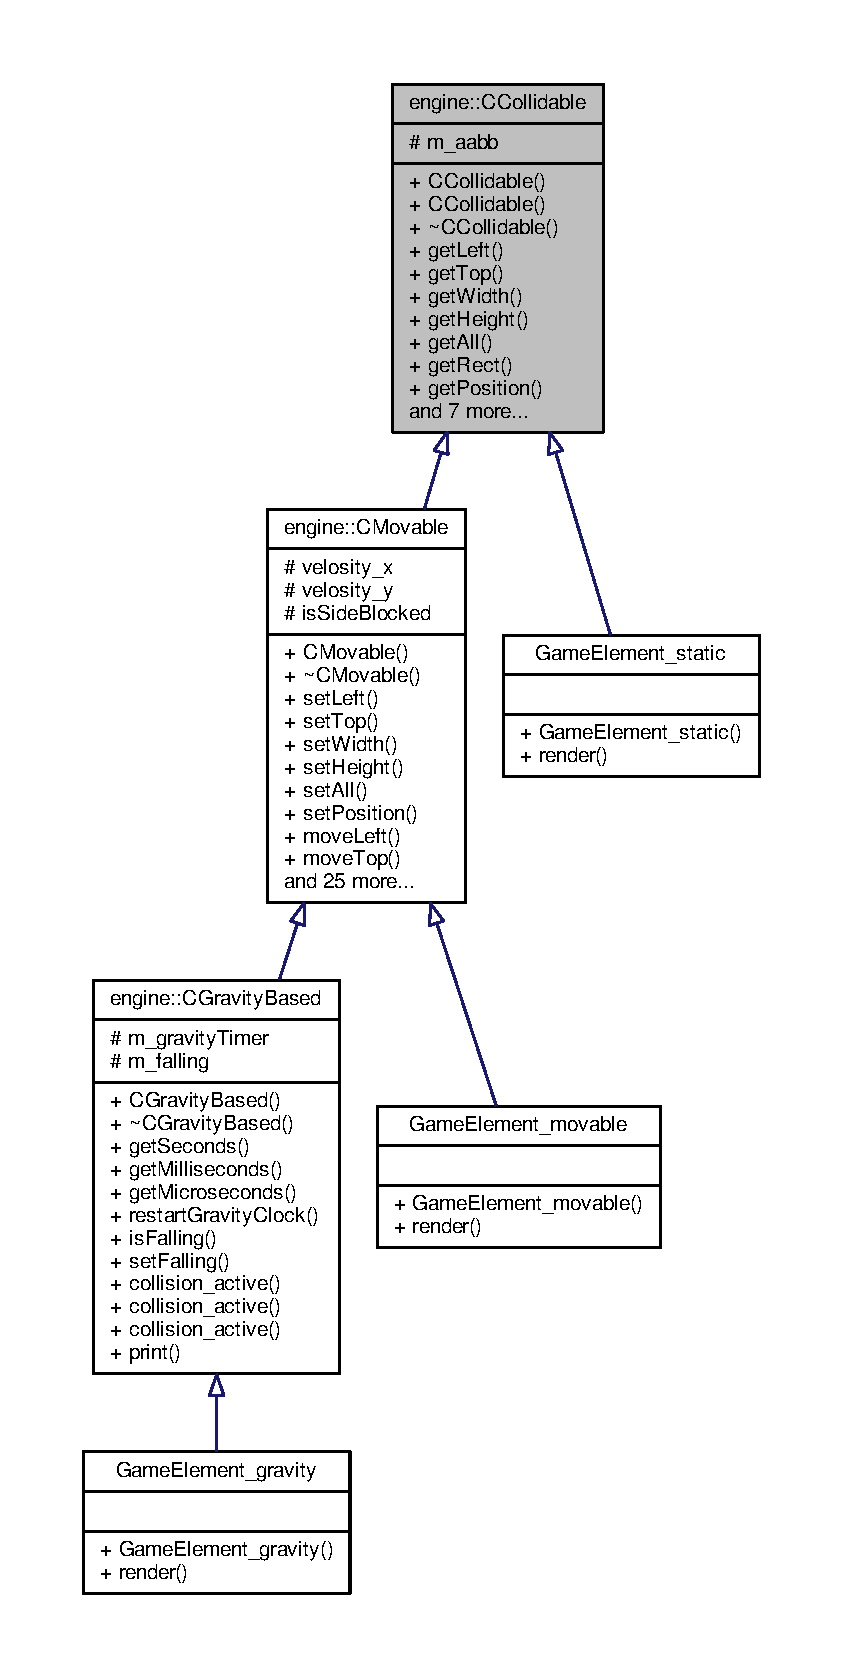
\includegraphics[height=550pt]{classengine_1_1CCollidable__inherit__graph}
\end{center}
\end{figure}


Collaboration diagram for engine\-:\-:C\-Collidable\-:
\nopagebreak
\begin{figure}[H]
\begin{center}
\leavevmode
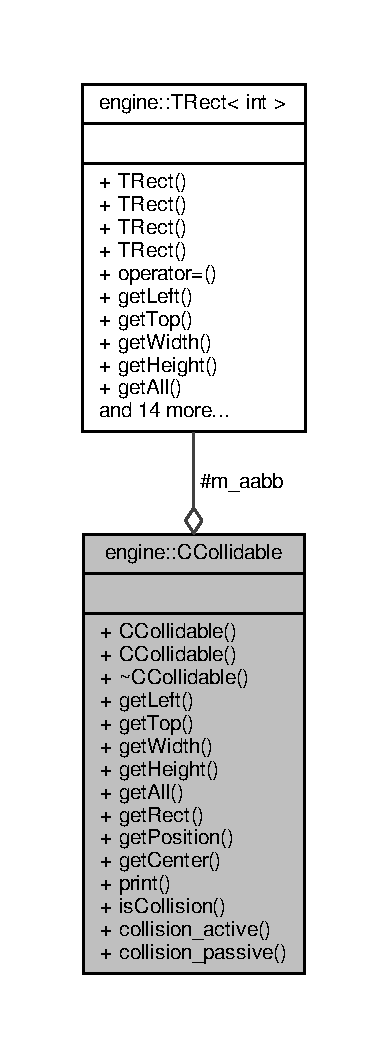
\includegraphics[width=186pt]{classengine_1_1CCollidable__coll__graph}
\end{center}
\end{figure}
\subsection*{Public Member Functions}
\begin{DoxyCompactItemize}
\item 
\hyperlink{classengine_1_1CCollidable_af462862c9147ddecb794456bac7d24af}{C\-Collidable} (\hyperlink{classCSprite}{C\-Sprite} $\ast$sprite)
\item 
\hyperlink{classengine_1_1CCollidable_a0cf5d0adac82ce344fa0a9944739d87b}{C\-Collidable} (const \hyperlink{classengine_1_1TRect}{T\-Rect}$<$ int $>$ $\ast$rect)
\item 
virtual \hyperlink{classengine_1_1CCollidable_aab6e393808cd5f3a6144889df36e9523}{$\sim$\-C\-Collidable} ()
\item 
int \hyperlink{classengine_1_1CCollidable_a4144d3b4711ae7570f6b122e5b4e1435}{get\-Left} () const 
\item 
int \hyperlink{classengine_1_1CCollidable_adb2d96cc98dc4b6ed5a26cd9129e1d2d}{get\-Top} () const 
\item 
int \hyperlink{classengine_1_1CCollidable_afba2923113db4ebde67912978885ec72}{get\-Width} () const 
\item 
int \hyperlink{classengine_1_1CCollidable_a6436c774e28bcbee83472f91c059283a}{get\-Height} () const 
\item 
void \hyperlink{classengine_1_1CCollidable_a0945e8a00846ff20ecdd86102afe04aa}{get\-All} (int \&left, int \&top, int \&width, int \&height) const 
\item 
void \hyperlink{classengine_1_1CCollidable_ae026a66abb2bfa169227255335d9f78b}{get\-Rect} (\hyperlink{classengine_1_1TRect}{T\-Rect}$<$ int $>$ $\ast$rect) const 
\item 
void \hyperlink{classengine_1_1CCollidable_a60fa629f81692094f135d01c2a4f5b69}{get\-Position} (int \&left, int \&top) const 
\item 
void \hyperlink{classengine_1_1CCollidable_a1855752c68f9d17856ce6c48234818fc}{get\-Center} (int \&x, int \&y) const 
\item 
virtual void \hyperlink{classengine_1_1CCollidable_a94c0157c8fdd9fccbfe8cdd726da2473}{print} () const 
\item 
bool \hyperlink{classengine_1_1CCollidable_afd5adee0a4b0a4f18ff2bdcda656c632}{is\-Collision} (const \hyperlink{classengine_1_1TRect}{T\-Rect}$<$ int $>$ $\ast$other\-\_\-rect) const 
\begin{DoxyCompactList}\small\item\em Does 'this' and 'other\-\_\-rect' intersect? \end{DoxyCompactList}\item 
virtual void \hyperlink{classengine_1_1CCollidable_abab887e8665ec79c153461eea5b7ea31}{collision\-\_\-active} ()
\item 
virtual void \hyperlink{classengine_1_1CCollidable_a610b5f5c85eeeee7e73d55a9c064353c}{collision\-\_\-passive} ()
\end{DoxyCompactItemize}
\subsection*{Protected Attributes}
\begin{DoxyCompactItemize}
\item 
\hyperlink{classengine_1_1TRect}{T\-Rect}$<$ int $>$ \hyperlink{classengine_1_1CCollidable_aca283a2f940e99dcd6b0f57e7812968d}{m\-\_\-aabb}
\begin{DoxyCompactList}\small\item\em Axis Aligned Bounding Box (A\-A\-B\-B), the thing that is the defined region of this object. \end{DoxyCompactList}\end{DoxyCompactItemize}


\subsection{Detailed Description}
The base class for all physics objects. 

Objects who inherit from this can collide with other \hyperlink{classengine_1_1CCollidable}{C\-Collidable} objects 

Definition at line 14 of file C\-Collidable.\-h.



\subsection{Constructor \& Destructor Documentation}
\hypertarget{classengine_1_1CCollidable_af462862c9147ddecb794456bac7d24af}{\index{engine\-::\-C\-Collidable@{engine\-::\-C\-Collidable}!C\-Collidable@{C\-Collidable}}
\index{C\-Collidable@{C\-Collidable}!engine::CCollidable@{engine\-::\-C\-Collidable}}
\subsubsection[{C\-Collidable}]{\setlength{\rightskip}{0pt plus 5cm}engine\-::\-C\-Collidable\-::\-C\-Collidable (
\begin{DoxyParamCaption}
\item[{{\bf C\-Sprite} $\ast$}]{sprite}
\end{DoxyParamCaption}
)}}\label{classengine_1_1CCollidable_af462862c9147ddecb794456bac7d24af}


Definition at line 8 of file C\-Collidable.\-cpp.

\hypertarget{classengine_1_1CCollidable_a0cf5d0adac82ce344fa0a9944739d87b}{\index{engine\-::\-C\-Collidable@{engine\-::\-C\-Collidable}!C\-Collidable@{C\-Collidable}}
\index{C\-Collidable@{C\-Collidable}!engine::CCollidable@{engine\-::\-C\-Collidable}}
\subsubsection[{C\-Collidable}]{\setlength{\rightskip}{0pt plus 5cm}engine\-::\-C\-Collidable\-::\-C\-Collidable (
\begin{DoxyParamCaption}
\item[{const {\bf T\-Rect}$<$ int $>$ $\ast$}]{rect}
\end{DoxyParamCaption}
)}}\label{classengine_1_1CCollidable_a0cf5d0adac82ce344fa0a9944739d87b}


Definition at line 14 of file C\-Collidable.\-cpp.

\hypertarget{classengine_1_1CCollidable_aab6e393808cd5f3a6144889df36e9523}{\index{engine\-::\-C\-Collidable@{engine\-::\-C\-Collidable}!$\sim$\-C\-Collidable@{$\sim$\-C\-Collidable}}
\index{$\sim$\-C\-Collidable@{$\sim$\-C\-Collidable}!engine::CCollidable@{engine\-::\-C\-Collidable}}
\subsubsection[{$\sim$\-C\-Collidable}]{\setlength{\rightskip}{0pt plus 5cm}engine\-::\-C\-Collidable\-::$\sim$\-C\-Collidable (
\begin{DoxyParamCaption}
{}
\end{DoxyParamCaption}
)\hspace{0.3cm}{\ttfamily [virtual]}}}\label{classengine_1_1CCollidable_aab6e393808cd5f3a6144889df36e9523}


Definition at line 21 of file C\-Collidable.\-cpp.



\subsection{Member Function Documentation}
\hypertarget{classengine_1_1CCollidable_abab887e8665ec79c153461eea5b7ea31}{\index{engine\-::\-C\-Collidable@{engine\-::\-C\-Collidable}!collision\-\_\-active@{collision\-\_\-active}}
\index{collision\-\_\-active@{collision\-\_\-active}!engine::CCollidable@{engine\-::\-C\-Collidable}}
\subsubsection[{collision\-\_\-active}]{\setlength{\rightskip}{0pt plus 5cm}void engine\-::\-C\-Collidable\-::collision\-\_\-active (
\begin{DoxyParamCaption}
{}
\end{DoxyParamCaption}
)\hspace{0.3cm}{\ttfamily [virtual]}}}\label{classengine_1_1CCollidable_abab887e8665ec79c153461eea5b7ea31}


Definition at line 128 of file C\-Collidable.\-cpp.

\hypertarget{classengine_1_1CCollidable_a610b5f5c85eeeee7e73d55a9c064353c}{\index{engine\-::\-C\-Collidable@{engine\-::\-C\-Collidable}!collision\-\_\-passive@{collision\-\_\-passive}}
\index{collision\-\_\-passive@{collision\-\_\-passive}!engine::CCollidable@{engine\-::\-C\-Collidable}}
\subsubsection[{collision\-\_\-passive}]{\setlength{\rightskip}{0pt plus 5cm}void engine\-::\-C\-Collidable\-::collision\-\_\-passive (
\begin{DoxyParamCaption}
{}
\end{DoxyParamCaption}
)\hspace{0.3cm}{\ttfamily [virtual]}}}\label{classengine_1_1CCollidable_a610b5f5c85eeeee7e73d55a9c064353c}


Definition at line 133 of file C\-Collidable.\-cpp.

\hypertarget{classengine_1_1CCollidable_a0945e8a00846ff20ecdd86102afe04aa}{\index{engine\-::\-C\-Collidable@{engine\-::\-C\-Collidable}!get\-All@{get\-All}}
\index{get\-All@{get\-All}!engine::CCollidable@{engine\-::\-C\-Collidable}}
\subsubsection[{get\-All}]{\setlength{\rightskip}{0pt plus 5cm}void engine\-::\-C\-Collidable\-::get\-All (
\begin{DoxyParamCaption}
\item[{int \&}]{left, }
\item[{int \&}]{top, }
\item[{int \&}]{width, }
\item[{int \&}]{height}
\end{DoxyParamCaption}
) const}}\label{classengine_1_1CCollidable_a0945e8a00846ff20ecdd86102afe04aa}


Definition at line 50 of file C\-Collidable.\-cpp.

\hypertarget{classengine_1_1CCollidable_a1855752c68f9d17856ce6c48234818fc}{\index{engine\-::\-C\-Collidable@{engine\-::\-C\-Collidable}!get\-Center@{get\-Center}}
\index{get\-Center@{get\-Center}!engine::CCollidable@{engine\-::\-C\-Collidable}}
\subsubsection[{get\-Center}]{\setlength{\rightskip}{0pt plus 5cm}void engine\-::\-C\-Collidable\-::get\-Center (
\begin{DoxyParamCaption}
\item[{int \&}]{x, }
\item[{int \&}]{y}
\end{DoxyParamCaption}
) const}}\label{classengine_1_1CCollidable_a1855752c68f9d17856ce6c48234818fc}


Definition at line 72 of file C\-Collidable.\-cpp.

\hypertarget{classengine_1_1CCollidable_a6436c774e28bcbee83472f91c059283a}{\index{engine\-::\-C\-Collidable@{engine\-::\-C\-Collidable}!get\-Height@{get\-Height}}
\index{get\-Height@{get\-Height}!engine::CCollidable@{engine\-::\-C\-Collidable}}
\subsubsection[{get\-Height}]{\setlength{\rightskip}{0pt plus 5cm}int engine\-::\-C\-Collidable\-::get\-Height (
\begin{DoxyParamCaption}
{}
\end{DoxyParamCaption}
) const}}\label{classengine_1_1CCollidable_a6436c774e28bcbee83472f91c059283a}


Definition at line 44 of file C\-Collidable.\-cpp.

\hypertarget{classengine_1_1CCollidable_a4144d3b4711ae7570f6b122e5b4e1435}{\index{engine\-::\-C\-Collidable@{engine\-::\-C\-Collidable}!get\-Left@{get\-Left}}
\index{get\-Left@{get\-Left}!engine::CCollidable@{engine\-::\-C\-Collidable}}
\subsubsection[{get\-Left}]{\setlength{\rightskip}{0pt plus 5cm}int engine\-::\-C\-Collidable\-::get\-Left (
\begin{DoxyParamCaption}
{}
\end{DoxyParamCaption}
) const}}\label{classengine_1_1CCollidable_a4144d3b4711ae7570f6b122e5b4e1435}


Definition at line 26 of file C\-Collidable.\-cpp.

\hypertarget{classengine_1_1CCollidable_a60fa629f81692094f135d01c2a4f5b69}{\index{engine\-::\-C\-Collidable@{engine\-::\-C\-Collidable}!get\-Position@{get\-Position}}
\index{get\-Position@{get\-Position}!engine::CCollidable@{engine\-::\-C\-Collidable}}
\subsubsection[{get\-Position}]{\setlength{\rightskip}{0pt plus 5cm}void engine\-::\-C\-Collidable\-::get\-Position (
\begin{DoxyParamCaption}
\item[{int \&}]{left, }
\item[{int \&}]{top}
\end{DoxyParamCaption}
) const}}\label{classengine_1_1CCollidable_a60fa629f81692094f135d01c2a4f5b69}


Definition at line 65 of file C\-Collidable.\-cpp.

\hypertarget{classengine_1_1CCollidable_ae026a66abb2bfa169227255335d9f78b}{\index{engine\-::\-C\-Collidable@{engine\-::\-C\-Collidable}!get\-Rect@{get\-Rect}}
\index{get\-Rect@{get\-Rect}!engine::CCollidable@{engine\-::\-C\-Collidable}}
\subsubsection[{get\-Rect}]{\setlength{\rightskip}{0pt plus 5cm}void engine\-::\-C\-Collidable\-::get\-Rect (
\begin{DoxyParamCaption}
\item[{{\bf T\-Rect}$<$ int $>$ $\ast$}]{rect}
\end{DoxyParamCaption}
) const}}\label{classengine_1_1CCollidable_ae026a66abb2bfa169227255335d9f78b}


Definition at line 59 of file C\-Collidable.\-cpp.

\hypertarget{classengine_1_1CCollidable_adb2d96cc98dc4b6ed5a26cd9129e1d2d}{\index{engine\-::\-C\-Collidable@{engine\-::\-C\-Collidable}!get\-Top@{get\-Top}}
\index{get\-Top@{get\-Top}!engine::CCollidable@{engine\-::\-C\-Collidable}}
\subsubsection[{get\-Top}]{\setlength{\rightskip}{0pt plus 5cm}int engine\-::\-C\-Collidable\-::get\-Top (
\begin{DoxyParamCaption}
{}
\end{DoxyParamCaption}
) const}}\label{classengine_1_1CCollidable_adb2d96cc98dc4b6ed5a26cd9129e1d2d}


Definition at line 32 of file C\-Collidable.\-cpp.

\hypertarget{classengine_1_1CCollidable_afba2923113db4ebde67912978885ec72}{\index{engine\-::\-C\-Collidable@{engine\-::\-C\-Collidable}!get\-Width@{get\-Width}}
\index{get\-Width@{get\-Width}!engine::CCollidable@{engine\-::\-C\-Collidable}}
\subsubsection[{get\-Width}]{\setlength{\rightskip}{0pt plus 5cm}int engine\-::\-C\-Collidable\-::get\-Width (
\begin{DoxyParamCaption}
{}
\end{DoxyParamCaption}
) const}}\label{classengine_1_1CCollidable_afba2923113db4ebde67912978885ec72}


Definition at line 38 of file C\-Collidable.\-cpp.

\hypertarget{classengine_1_1CCollidable_afd5adee0a4b0a4f18ff2bdcda656c632}{\index{engine\-::\-C\-Collidable@{engine\-::\-C\-Collidable}!is\-Collision@{is\-Collision}}
\index{is\-Collision@{is\-Collision}!engine::CCollidable@{engine\-::\-C\-Collidable}}
\subsubsection[{is\-Collision}]{\setlength{\rightskip}{0pt plus 5cm}bool engine\-::\-C\-Collidable\-::is\-Collision (
\begin{DoxyParamCaption}
\item[{const {\bf T\-Rect}$<$ int $>$ $\ast$}]{other\-\_\-rect}
\end{DoxyParamCaption}
) const}}\label{classengine_1_1CCollidable_afd5adee0a4b0a4f18ff2bdcda656c632}


Does 'this' and 'other\-\_\-rect' intersect? 

Note\-: the equals to in the equalities means that being 1 pixel away is not a collision, ie a ray-\/cast through it will not pass, but they are not colliding

Definition at line 84 of file C\-Collidable.\-cpp.

\hypertarget{classengine_1_1CCollidable_a94c0157c8fdd9fccbfe8cdd726da2473}{\index{engine\-::\-C\-Collidable@{engine\-::\-C\-Collidable}!print@{print}}
\index{print@{print}!engine::CCollidable@{engine\-::\-C\-Collidable}}
\subsubsection[{print}]{\setlength{\rightskip}{0pt plus 5cm}void engine\-::\-C\-Collidable\-::print (
\begin{DoxyParamCaption}
{}
\end{DoxyParamCaption}
) const\hspace{0.3cm}{\ttfamily [virtual]}}}\label{classengine_1_1CCollidable_a94c0157c8fdd9fccbfe8cdd726da2473}


Reimplemented in \hyperlink{classengine_1_1CMovable_a18299a0373464c4e1aadcdc9824eed9a}{engine\-::\-C\-Movable}.



Definition at line 78 of file C\-Collidable.\-cpp.



\subsection{Member Data Documentation}
\hypertarget{classengine_1_1CCollidable_aca283a2f940e99dcd6b0f57e7812968d}{\index{engine\-::\-C\-Collidable@{engine\-::\-C\-Collidable}!m\-\_\-aabb@{m\-\_\-aabb}}
\index{m\-\_\-aabb@{m\-\_\-aabb}!engine::CCollidable@{engine\-::\-C\-Collidable}}
\subsubsection[{m\-\_\-aabb}]{\setlength{\rightskip}{0pt plus 5cm}{\bf T\-Rect}$<$int$>$ engine\-::\-C\-Collidable\-::m\-\_\-aabb\hspace{0.3cm}{\ttfamily [protected]}}}\label{classengine_1_1CCollidable_aca283a2f940e99dcd6b0f57e7812968d}


Axis Aligned Bounding Box (A\-A\-B\-B), the thing that is the defined region of this object. 



Definition at line 45 of file C\-Collidable.\-h.



The documentation for this class was generated from the following files\-:\begin{DoxyCompactItemize}
\item 
/home/z\-Zelman/\-Dropbox/2\-D-\/\-Game\-Engine/src/\-Physics/\hyperlink{CCollidable_8h}{C\-Collidable.\-h}\item 
/home/z\-Zelman/\-Dropbox/2\-D-\/\-Game\-Engine/src/\-Physics/\hyperlink{CCollidable_8cpp}{C\-Collidable.\-cpp}\end{DoxyCompactItemize}

\hypertarget{classengine_1_1CMovable}{\section{engine\-:\-:C\-Movable Class Reference}
\label{classengine_1_1CMovable}\index{engine\-::\-C\-Movable@{engine\-::\-C\-Movable}}
}


{\ttfamily \#include $<$C\-Movable.\-h$>$}



Inheritance diagram for engine\-:\-:C\-Movable\-:\nopagebreak
\begin{figure}[H]
\begin{center}
\leavevmode
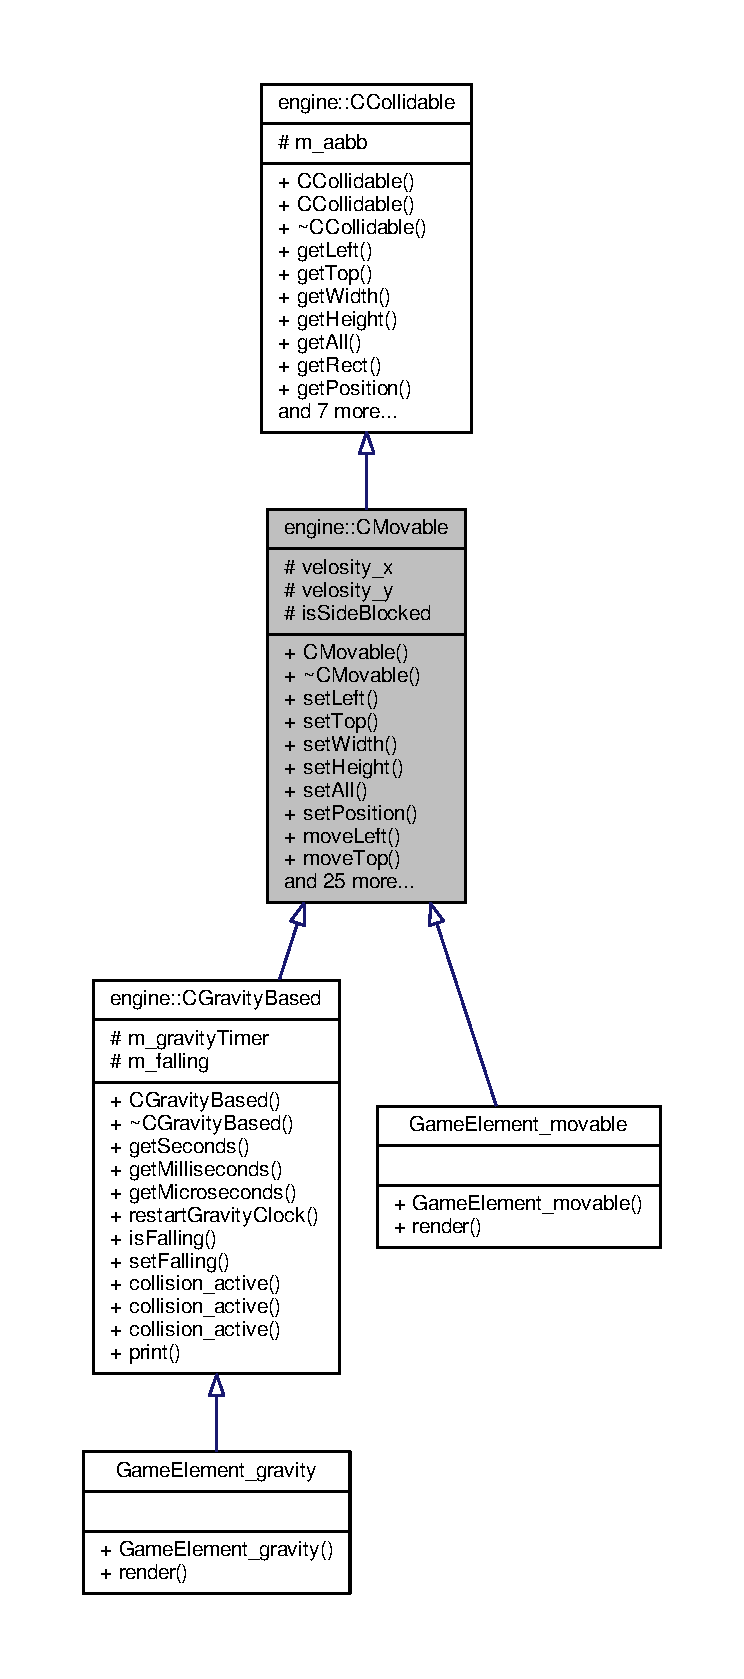
\includegraphics[height=550pt]{classengine_1_1CMovable__inherit__graph}
\end{center}
\end{figure}


Collaboration diagram for engine\-:\-:C\-Movable\-:\nopagebreak
\begin{figure}[H]
\begin{center}
\leavevmode
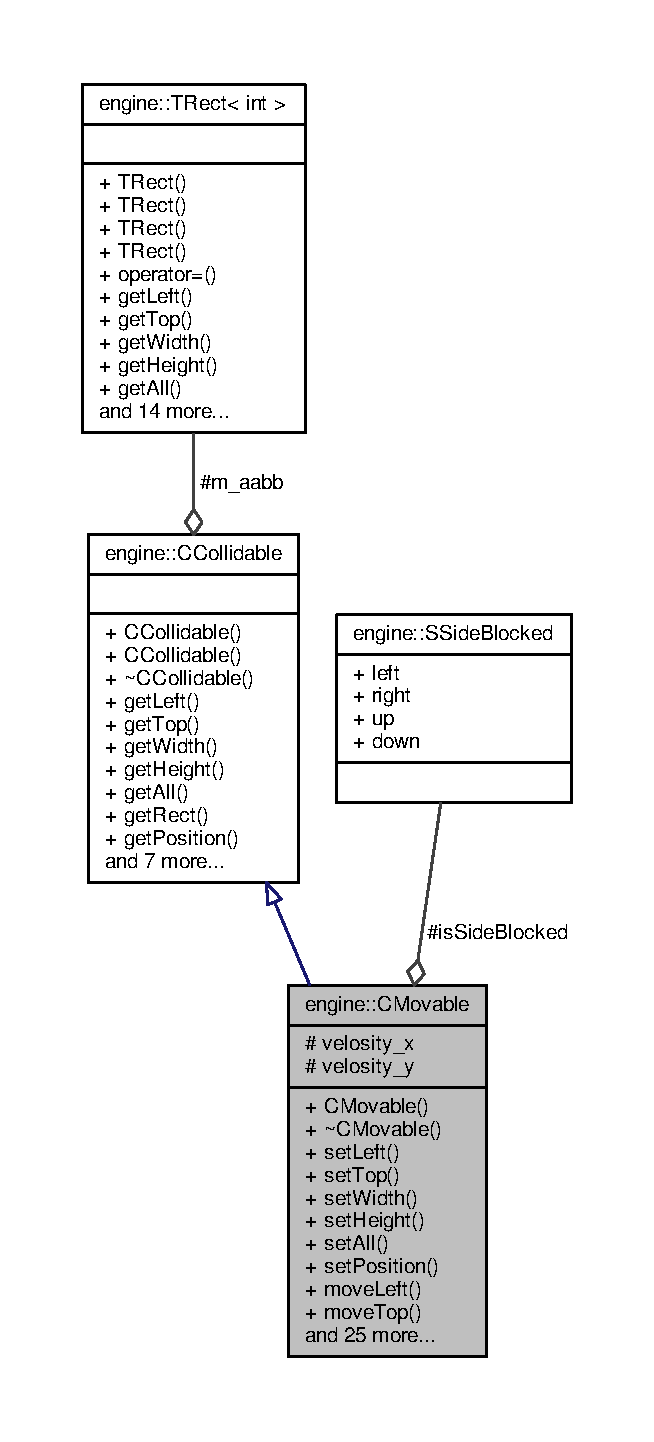
\includegraphics[height=550pt]{classengine_1_1CMovable__coll__graph}
\end{center}
\end{figure}
\subsection*{Public Member Functions}
\begin{DoxyCompactItemize}
\item 
\hyperlink{classengine_1_1CMovable_af28d9429a4bf12fc37fb807bb0ae9c05}{C\-Movable} (\hyperlink{classCSprite}{C\-Sprite} $\ast$sprite)
\item 
virtual \hyperlink{classengine_1_1CMovable_a2a8adce4d82128afdde96d0c9eb724b7}{$\sim$\-C\-Movable} ()
\item 
void \hyperlink{classengine_1_1CMovable_aa4b25f57e8b5613035463f28eaa4fc36}{set\-Left} (int left)
\item 
void \hyperlink{classengine_1_1CMovable_a680ee306f10a10a79616e3483300edb0}{set\-Top} (int top)
\item 
void \hyperlink{classengine_1_1CMovable_af8a646f2cebafb3f1cec4934132e3128}{set\-Width} (int width)
\item 
void \hyperlink{classengine_1_1CMovable_a6e78d43b1968931da9c91e4657502025}{set\-Height} (int height)
\item 
void \hyperlink{classengine_1_1CMovable_a98ef52dedd948dc2cc6fd5cad92444c0}{set\-All} (int left, int top, int width, int height)
\item 
void \hyperlink{classengine_1_1CMovable_ad6342adfc04b24120e5b19cf77fe44f5}{set\-Position} (int left, int top)
\item 
void \hyperlink{classengine_1_1CMovable_aba30b69bd14b16076f3d11c7b0471b83}{move\-Left} (int d\-\_\-left)
\item 
void \hyperlink{classengine_1_1CMovable_ad8f9971aa2d8c6a056d9ca04a2aba195}{move\-Top} (int d\-\_\-top)
\item 
void \hyperlink{classengine_1_1CMovable_a680b7faa861881cca82952f01d0fb20e}{move\-Position} (int d\-\_\-left, int d\-\_\-top)
\item 
void \hyperlink{classengine_1_1CMovable_aa9c441a7c6ea04959db6968f78dd9158}{get\-Velosity\-\_\-x} (float \&x) const 
\item 
void \hyperlink{classengine_1_1CMovable_a082d0f378616726256e96724c3009493}{get\-Velosity\-\_\-y} (float \&y) const 
\item 
void \hyperlink{classengine_1_1CMovable_a7fa5504cad44efed5da9cc2298bed93b}{get\-Velosity} (float \&x, float \&y) const 
\item 
void \hyperlink{classengine_1_1CMovable_a9f1674b45a63529f2cf1bcbfd65c1a28}{set\-Velosity\-\_\-x} (float x)
\item 
void \hyperlink{classengine_1_1CMovable_ac1ed31991776939ada3d50e551017ab4}{set\-Velosity\-\_\-y} (float y)
\item 
void \hyperlink{classengine_1_1CMovable_a5e7a42eb65b12035d2c6104f28f2f0fc}{set\-Velosity} (float x, float y)
\item 
void \hyperlink{classengine_1_1CMovable_a5774652cd5369fad6b08cf4de56f91c0}{get\-Is\-Side\-Blocked\-\_\-left} (bool \&left) const 
\item 
void \hyperlink{classengine_1_1CMovable_a7790f286b529e31de0226f72c574faef}{get\-Is\-Side\-Blocked\-\_\-right} (bool \&right) const 
\item 
void \hyperlink{classengine_1_1CMovable_a542748edb84d3e43bb479278c8b38e06}{get\-Is\-Side\-Blocked\-\_\-up} (bool \&up) const 
\item 
void \hyperlink{classengine_1_1CMovable_a85d5cf13541670517f1a49d57d49107a}{get\-Is\-Side\-Blocked\-\_\-down} (bool \&down) const 
\item 
void \hyperlink{classengine_1_1CMovable_a7252ea478abaab25c1774ccfd1f52554}{get\-Is\-Side\-Blocked} (\hyperlink{structengine_1_1SSideBlocked}{S\-Side\-Blocked} \&s) const 
\item 
void \hyperlink{classengine_1_1CMovable_a19c9b69038fe22d0a08228b7eaed8c1b}{get\-Is\-Side\-Blocked} (bool \&left, bool \&right, bool \&up, bool \&down) const 
\item 
void \hyperlink{classengine_1_1CMovable_aa7f9177dee6821517c845f1d369f8cde}{set\-Is\-Side\-Blocked\-\_\-left} (bool left)
\item 
void \hyperlink{classengine_1_1CMovable_af1059fe2fbaf39598efe0a234d8cbc9e}{set\-Is\-Side\-Blocked\-\_\-right} (bool right)
\item 
void \hyperlink{classengine_1_1CMovable_a73ec50c7ed0037c4abe4aaa41ffe68d7}{set\-Is\-Side\-Blocked\-\_\-up} (bool up)
\item 
void \hyperlink{classengine_1_1CMovable_a454f67c854ad8f16c7251bc1011a2673}{set\-Is\-Side\-Blocked\-\_\-down} (bool down)
\item 
void \hyperlink{classengine_1_1CMovable_aafcffa645994fb19515bcb84cf083c9f}{set\-Is\-Side\-Blocked} (\hyperlink{structengine_1_1SSideBlocked}{S\-Side\-Blocked} s)
\item 
void \hyperlink{classengine_1_1CMovable_a61e5537f10e7ff0f111c1ad355f0f6ed}{set\-Is\-Side\-Blocked} (bool left, bool right, bool up, bool down)
\item 
virtual void \hyperlink{classengine_1_1CMovable_a6184018afcab4be164c3b02228175a9c}{move\-\_\-normally} ()
\begin{DoxyCompactList}\small\item\em Update position based on x and y velocities. \end{DoxyCompactList}\item 
void \hyperlink{classengine_1_1CMovable_a9643f34424f25ec389cb784c84988f14}{determine\-\_\-side\-Blocked} (\hyperlink{classengine_1_1CCollidable}{C\-Collidable} $\ast$c)
\begin{DoxyCompactList}\small\item\em Given the \hyperlink{classengine_1_1CCollidable}{C\-Collidable} object, does it block one of your sides? \end{DoxyCompactList}\item 
virtual void \hyperlink{classengine_1_1CMovable_a7ac299dcc08c6c783b2d77ec665041f4}{collision\-\_\-active} (\hyperlink{classengine_1_1CCollidable}{C\-Collidable} $\ast$c)
\item 
virtual void \hyperlink{classengine_1_1CMovable_ad04d949e3d7e2e182df9fbffae48ecd8}{collision\-\_\-active} (\hyperlink{classengine_1_1CMovable}{C\-Movable} $\ast$m)
\item 
virtual void \hyperlink{classengine_1_1CMovable_ae4173fad2cbd60a3929c42aee9916cb4}{collision\-\_\-active} (\hyperlink{classengine_1_1CGravityBased}{C\-Gravity\-Based} $\ast$g)
\item 
virtual void \hyperlink{classengine_1_1CMovable_a18299a0373464c4e1aadcdc9824eed9a}{print} () const 
\end{DoxyCompactItemize}
\subsection*{Protected Attributes}
\begin{DoxyCompactItemize}
\item 
float \hyperlink{classengine_1_1CMovable_a7bc34defa8ea4190a6c3011ef254e48b}{velosity\-\_\-x}
\item 
float \hyperlink{classengine_1_1CMovable_a7a1a4581926122ae31753261d1d35cf3}{velosity\-\_\-y}
\item 
struct \hyperlink{structengine_1_1SSideBlocked}{S\-Side\-Blocked} \hyperlink{classengine_1_1CMovable_afa7eb7bff0a1475aab175c9de7cd428a}{is\-Side\-Blocked}
\begin{DoxyCompactList}\small\item\em Blocked == true. \end{DoxyCompactList}\end{DoxyCompactItemize}


\subsection{Detailed Description}


Definition at line 19 of file C\-Movable.\-h.



\subsection{Constructor \& Destructor Documentation}
\hypertarget{classengine_1_1CMovable_af28d9429a4bf12fc37fb807bb0ae9c05}{\index{engine\-::\-C\-Movable@{engine\-::\-C\-Movable}!C\-Movable@{C\-Movable}}
\index{C\-Movable@{C\-Movable}!engine::CMovable@{engine\-::\-C\-Movable}}
\subsubsection[{C\-Movable}]{\setlength{\rightskip}{0pt plus 5cm}engine\-::\-C\-Movable\-::\-C\-Movable (
\begin{DoxyParamCaption}
\item[{{\bf C\-Sprite} $\ast$}]{sprite}
\end{DoxyParamCaption}
)}}\label{classengine_1_1CMovable_af28d9429a4bf12fc37fb807bb0ae9c05}


Definition at line 9 of file C\-Movable.\-cpp.

\hypertarget{classengine_1_1CMovable_a2a8adce4d82128afdde96d0c9eb724b7}{\index{engine\-::\-C\-Movable@{engine\-::\-C\-Movable}!$\sim$\-C\-Movable@{$\sim$\-C\-Movable}}
\index{$\sim$\-C\-Movable@{$\sim$\-C\-Movable}!engine::CMovable@{engine\-::\-C\-Movable}}
\subsubsection[{$\sim$\-C\-Movable}]{\setlength{\rightskip}{0pt plus 5cm}engine\-::\-C\-Movable\-::$\sim$\-C\-Movable (
\begin{DoxyParamCaption}
{}
\end{DoxyParamCaption}
)\hspace{0.3cm}{\ttfamily [virtual]}}}\label{classengine_1_1CMovable_a2a8adce4d82128afdde96d0c9eb724b7}


Definition at line 19 of file C\-Movable.\-cpp.



\subsection{Member Function Documentation}
\hypertarget{classengine_1_1CMovable_a7ac299dcc08c6c783b2d77ec665041f4}{\index{engine\-::\-C\-Movable@{engine\-::\-C\-Movable}!collision\-\_\-active@{collision\-\_\-active}}
\index{collision\-\_\-active@{collision\-\_\-active}!engine::CMovable@{engine\-::\-C\-Movable}}
\subsubsection[{collision\-\_\-active}]{\setlength{\rightskip}{0pt plus 5cm}void engine\-::\-C\-Movable\-::collision\-\_\-active (
\begin{DoxyParamCaption}
\item[{{\bf C\-Collidable} $\ast$}]{c}
\end{DoxyParamCaption}
)\hspace{0.3cm}{\ttfamily [virtual]}}}\label{classengine_1_1CMovable_a7ac299dcc08c6c783b2d77ec665041f4}


Reimplemented in \hyperlink{classengine_1_1CGravityBased_aedf5cefc210d802cd219366b30ced9f8}{engine\-::\-C\-Gravity\-Based}.



Definition at line 267 of file C\-Movable.\-cpp.

\hypertarget{classengine_1_1CMovable_ad04d949e3d7e2e182df9fbffae48ecd8}{\index{engine\-::\-C\-Movable@{engine\-::\-C\-Movable}!collision\-\_\-active@{collision\-\_\-active}}
\index{collision\-\_\-active@{collision\-\_\-active}!engine::CMovable@{engine\-::\-C\-Movable}}
\subsubsection[{collision\-\_\-active}]{\setlength{\rightskip}{0pt plus 5cm}void engine\-::\-C\-Movable\-::collision\-\_\-active (
\begin{DoxyParamCaption}
\item[{{\bf C\-Movable} $\ast$}]{m}
\end{DoxyParamCaption}
)\hspace{0.3cm}{\ttfamily [virtual]}}}\label{classengine_1_1CMovable_ad04d949e3d7e2e182df9fbffae48ecd8}


Reimplemented in \hyperlink{classengine_1_1CGravityBased_a47f5f1081f356b4941401e0648a2a3f9}{engine\-::\-C\-Gravity\-Based}.



Definition at line 274 of file C\-Movable.\-cpp.

\hypertarget{classengine_1_1CMovable_ae4173fad2cbd60a3929c42aee9916cb4}{\index{engine\-::\-C\-Movable@{engine\-::\-C\-Movable}!collision\-\_\-active@{collision\-\_\-active}}
\index{collision\-\_\-active@{collision\-\_\-active}!engine::CMovable@{engine\-::\-C\-Movable}}
\subsubsection[{collision\-\_\-active}]{\setlength{\rightskip}{0pt plus 5cm}void engine\-::\-C\-Movable\-::collision\-\_\-active (
\begin{DoxyParamCaption}
\item[{{\bf C\-Gravity\-Based} $\ast$}]{g}
\end{DoxyParamCaption}
)\hspace{0.3cm}{\ttfamily [virtual]}}}\label{classengine_1_1CMovable_ae4173fad2cbd60a3929c42aee9916cb4}


Reimplemented in \hyperlink{classengine_1_1CGravityBased_ac04bb2389041ba872a22cd575ae52dd6}{engine\-::\-C\-Gravity\-Based}.



Definition at line 281 of file C\-Movable.\-cpp.

\hypertarget{classengine_1_1CMovable_a9643f34424f25ec389cb784c84988f14}{\index{engine\-::\-C\-Movable@{engine\-::\-C\-Movable}!determine\-\_\-side\-Blocked@{determine\-\_\-side\-Blocked}}
\index{determine\-\_\-side\-Blocked@{determine\-\_\-side\-Blocked}!engine::CMovable@{engine\-::\-C\-Movable}}
\subsubsection[{determine\-\_\-side\-Blocked}]{\setlength{\rightskip}{0pt plus 5cm}void engine\-::\-C\-Movable\-::determine\-\_\-side\-Blocked (
\begin{DoxyParamCaption}
\item[{{\bf C\-Collidable} $\ast$}]{c}
\end{DoxyParamCaption}
)}}\label{classengine_1_1CMovable_a9643f34424f25ec389cb784c84988f14}


Given the \hyperlink{classengine_1_1CCollidable}{C\-Collidable} object, does it block one of your sides? 



Definition at line 232 of file C\-Movable.\-cpp.

\hypertarget{classengine_1_1CMovable_a7252ea478abaab25c1774ccfd1f52554}{\index{engine\-::\-C\-Movable@{engine\-::\-C\-Movable}!get\-Is\-Side\-Blocked@{get\-Is\-Side\-Blocked}}
\index{get\-Is\-Side\-Blocked@{get\-Is\-Side\-Blocked}!engine::CMovable@{engine\-::\-C\-Movable}}
\subsubsection[{get\-Is\-Side\-Blocked}]{\setlength{\rightskip}{0pt plus 5cm}void engine\-::\-C\-Movable\-::get\-Is\-Side\-Blocked (
\begin{DoxyParamCaption}
\item[{{\bf S\-Side\-Blocked} \&}]{s}
\end{DoxyParamCaption}
) const}}\label{classengine_1_1CMovable_a7252ea478abaab25c1774ccfd1f52554}


Definition at line 167 of file C\-Movable.\-cpp.

\hypertarget{classengine_1_1CMovable_a19c9b69038fe22d0a08228b7eaed8c1b}{\index{engine\-::\-C\-Movable@{engine\-::\-C\-Movable}!get\-Is\-Side\-Blocked@{get\-Is\-Side\-Blocked}}
\index{get\-Is\-Side\-Blocked@{get\-Is\-Side\-Blocked}!engine::CMovable@{engine\-::\-C\-Movable}}
\subsubsection[{get\-Is\-Side\-Blocked}]{\setlength{\rightskip}{0pt plus 5cm}void engine\-::\-C\-Movable\-::get\-Is\-Side\-Blocked (
\begin{DoxyParamCaption}
\item[{bool \&}]{left, }
\item[{bool \&}]{right, }
\item[{bool \&}]{up, }
\item[{bool \&}]{down}
\end{DoxyParamCaption}
) const}}\label{classengine_1_1CMovable_a19c9b69038fe22d0a08228b7eaed8c1b}


Definition at line 175 of file C\-Movable.\-cpp.

\hypertarget{classengine_1_1CMovable_a85d5cf13541670517f1a49d57d49107a}{\index{engine\-::\-C\-Movable@{engine\-::\-C\-Movable}!get\-Is\-Side\-Blocked\-\_\-down@{get\-Is\-Side\-Blocked\-\_\-down}}
\index{get\-Is\-Side\-Blocked\-\_\-down@{get\-Is\-Side\-Blocked\-\_\-down}!engine::CMovable@{engine\-::\-C\-Movable}}
\subsubsection[{get\-Is\-Side\-Blocked\-\_\-down}]{\setlength{\rightskip}{0pt plus 5cm}void engine\-::\-C\-Movable\-::get\-Is\-Side\-Blocked\-\_\-down (
\begin{DoxyParamCaption}
\item[{bool \&}]{down}
\end{DoxyParamCaption}
) const}}\label{classengine_1_1CMovable_a85d5cf13541670517f1a49d57d49107a}


Definition at line 161 of file C\-Movable.\-cpp.

\hypertarget{classengine_1_1CMovable_a5774652cd5369fad6b08cf4de56f91c0}{\index{engine\-::\-C\-Movable@{engine\-::\-C\-Movable}!get\-Is\-Side\-Blocked\-\_\-left@{get\-Is\-Side\-Blocked\-\_\-left}}
\index{get\-Is\-Side\-Blocked\-\_\-left@{get\-Is\-Side\-Blocked\-\_\-left}!engine::CMovable@{engine\-::\-C\-Movable}}
\subsubsection[{get\-Is\-Side\-Blocked\-\_\-left}]{\setlength{\rightskip}{0pt plus 5cm}void engine\-::\-C\-Movable\-::get\-Is\-Side\-Blocked\-\_\-left (
\begin{DoxyParamCaption}
\item[{bool \&}]{left}
\end{DoxyParamCaption}
) const}}\label{classengine_1_1CMovable_a5774652cd5369fad6b08cf4de56f91c0}


Definition at line 143 of file C\-Movable.\-cpp.

\hypertarget{classengine_1_1CMovable_a7790f286b529e31de0226f72c574faef}{\index{engine\-::\-C\-Movable@{engine\-::\-C\-Movable}!get\-Is\-Side\-Blocked\-\_\-right@{get\-Is\-Side\-Blocked\-\_\-right}}
\index{get\-Is\-Side\-Blocked\-\_\-right@{get\-Is\-Side\-Blocked\-\_\-right}!engine::CMovable@{engine\-::\-C\-Movable}}
\subsubsection[{get\-Is\-Side\-Blocked\-\_\-right}]{\setlength{\rightskip}{0pt plus 5cm}void engine\-::\-C\-Movable\-::get\-Is\-Side\-Blocked\-\_\-right (
\begin{DoxyParamCaption}
\item[{bool \&}]{right}
\end{DoxyParamCaption}
) const}}\label{classengine_1_1CMovable_a7790f286b529e31de0226f72c574faef}


Definition at line 149 of file C\-Movable.\-cpp.

\hypertarget{classengine_1_1CMovable_a542748edb84d3e43bb479278c8b38e06}{\index{engine\-::\-C\-Movable@{engine\-::\-C\-Movable}!get\-Is\-Side\-Blocked\-\_\-up@{get\-Is\-Side\-Blocked\-\_\-up}}
\index{get\-Is\-Side\-Blocked\-\_\-up@{get\-Is\-Side\-Blocked\-\_\-up}!engine::CMovable@{engine\-::\-C\-Movable}}
\subsubsection[{get\-Is\-Side\-Blocked\-\_\-up}]{\setlength{\rightskip}{0pt plus 5cm}void engine\-::\-C\-Movable\-::get\-Is\-Side\-Blocked\-\_\-up (
\begin{DoxyParamCaption}
\item[{bool \&}]{up}
\end{DoxyParamCaption}
) const}}\label{classengine_1_1CMovable_a542748edb84d3e43bb479278c8b38e06}


Definition at line 155 of file C\-Movable.\-cpp.

\hypertarget{classengine_1_1CMovable_a7fa5504cad44efed5da9cc2298bed93b}{\index{engine\-::\-C\-Movable@{engine\-::\-C\-Movable}!get\-Velosity@{get\-Velosity}}
\index{get\-Velosity@{get\-Velosity}!engine::CMovable@{engine\-::\-C\-Movable}}
\subsubsection[{get\-Velosity}]{\setlength{\rightskip}{0pt plus 5cm}void engine\-::\-C\-Movable\-::get\-Velosity (
\begin{DoxyParamCaption}
\item[{float \&}]{x, }
\item[{float \&}]{y}
\end{DoxyParamCaption}
) const}}\label{classengine_1_1CMovable_a7fa5504cad44efed5da9cc2298bed93b}


Definition at line 117 of file C\-Movable.\-cpp.

\hypertarget{classengine_1_1CMovable_aa9c441a7c6ea04959db6968f78dd9158}{\index{engine\-::\-C\-Movable@{engine\-::\-C\-Movable}!get\-Velosity\-\_\-x@{get\-Velosity\-\_\-x}}
\index{get\-Velosity\-\_\-x@{get\-Velosity\-\_\-x}!engine::CMovable@{engine\-::\-C\-Movable}}
\subsubsection[{get\-Velosity\-\_\-x}]{\setlength{\rightskip}{0pt plus 5cm}void engine\-::\-C\-Movable\-::get\-Velosity\-\_\-x (
\begin{DoxyParamCaption}
\item[{float \&}]{x}
\end{DoxyParamCaption}
) const}}\label{classengine_1_1CMovable_aa9c441a7c6ea04959db6968f78dd9158}


Definition at line 105 of file C\-Movable.\-cpp.

\hypertarget{classengine_1_1CMovable_a082d0f378616726256e96724c3009493}{\index{engine\-::\-C\-Movable@{engine\-::\-C\-Movable}!get\-Velosity\-\_\-y@{get\-Velosity\-\_\-y}}
\index{get\-Velosity\-\_\-y@{get\-Velosity\-\_\-y}!engine::CMovable@{engine\-::\-C\-Movable}}
\subsubsection[{get\-Velosity\-\_\-y}]{\setlength{\rightskip}{0pt plus 5cm}void engine\-::\-C\-Movable\-::get\-Velosity\-\_\-y (
\begin{DoxyParamCaption}
\item[{float \&}]{y}
\end{DoxyParamCaption}
) const}}\label{classengine_1_1CMovable_a082d0f378616726256e96724c3009493}


Definition at line 111 of file C\-Movable.\-cpp.

\hypertarget{classengine_1_1CMovable_a6184018afcab4be164c3b02228175a9c}{\index{engine\-::\-C\-Movable@{engine\-::\-C\-Movable}!move\-\_\-normally@{move\-\_\-normally}}
\index{move\-\_\-normally@{move\-\_\-normally}!engine::CMovable@{engine\-::\-C\-Movable}}
\subsubsection[{move\-\_\-normally}]{\setlength{\rightskip}{0pt plus 5cm}void engine\-::\-C\-Movable\-::move\-\_\-normally (
\begin{DoxyParamCaption}
{}
\end{DoxyParamCaption}
)\hspace{0.3cm}{\ttfamily [virtual]}}}\label{classengine_1_1CMovable_a6184018afcab4be164c3b02228175a9c}


Update position based on x and y velocities. 



Definition at line 226 of file C\-Movable.\-cpp.

\hypertarget{classengine_1_1CMovable_aba30b69bd14b16076f3d11c7b0471b83}{\index{engine\-::\-C\-Movable@{engine\-::\-C\-Movable}!move\-Left@{move\-Left}}
\index{move\-Left@{move\-Left}!engine::CMovable@{engine\-::\-C\-Movable}}
\subsubsection[{move\-Left}]{\setlength{\rightskip}{0pt plus 5cm}void engine\-::\-C\-Movable\-::move\-Left (
\begin{DoxyParamCaption}
\item[{int}]{d\-\_\-left}
\end{DoxyParamCaption}
)}}\label{classengine_1_1CMovable_aba30b69bd14b16076f3d11c7b0471b83}


Definition at line 76 of file C\-Movable.\-cpp.

\hypertarget{classengine_1_1CMovable_a680b7faa861881cca82952f01d0fb20e}{\index{engine\-::\-C\-Movable@{engine\-::\-C\-Movable}!move\-Position@{move\-Position}}
\index{move\-Position@{move\-Position}!engine::CMovable@{engine\-::\-C\-Movable}}
\subsubsection[{move\-Position}]{\setlength{\rightskip}{0pt plus 5cm}void engine\-::\-C\-Movable\-::move\-Position (
\begin{DoxyParamCaption}
\item[{int}]{d\-\_\-left, }
\item[{int}]{d\-\_\-top}
\end{DoxyParamCaption}
)}}\label{classengine_1_1CMovable_a680b7faa861881cca82952f01d0fb20e}


Definition at line 98 of file C\-Movable.\-cpp.

\hypertarget{classengine_1_1CMovable_ad8f9971aa2d8c6a056d9ca04a2aba195}{\index{engine\-::\-C\-Movable@{engine\-::\-C\-Movable}!move\-Top@{move\-Top}}
\index{move\-Top@{move\-Top}!engine::CMovable@{engine\-::\-C\-Movable}}
\subsubsection[{move\-Top}]{\setlength{\rightskip}{0pt plus 5cm}void engine\-::\-C\-Movable\-::move\-Top (
\begin{DoxyParamCaption}
\item[{int}]{d\-\_\-top}
\end{DoxyParamCaption}
)}}\label{classengine_1_1CMovable_ad8f9971aa2d8c6a056d9ca04a2aba195}


Definition at line 87 of file C\-Movable.\-cpp.

\hypertarget{classengine_1_1CMovable_a18299a0373464c4e1aadcdc9824eed9a}{\index{engine\-::\-C\-Movable@{engine\-::\-C\-Movable}!print@{print}}
\index{print@{print}!engine::CMovable@{engine\-::\-C\-Movable}}
\subsubsection[{print}]{\setlength{\rightskip}{0pt plus 5cm}void engine\-::\-C\-Movable\-::print (
\begin{DoxyParamCaption}
{}
\end{DoxyParamCaption}
) const\hspace{0.3cm}{\ttfamily [virtual]}}}\label{classengine_1_1CMovable_a18299a0373464c4e1aadcdc9824eed9a}


Reimplemented from \hyperlink{classengine_1_1CCollidable_a94c0157c8fdd9fccbfe8cdd726da2473}{engine\-::\-C\-Collidable}.



Reimplemented in \hyperlink{classengine_1_1CGravityBased_a1fd898d6529eeb9bb8651d7d9bcdb89c}{engine\-::\-C\-Gravity\-Based}.



Definition at line 288 of file C\-Movable.\-cpp.

\hypertarget{classengine_1_1CMovable_a98ef52dedd948dc2cc6fd5cad92444c0}{\index{engine\-::\-C\-Movable@{engine\-::\-C\-Movable}!set\-All@{set\-All}}
\index{set\-All@{set\-All}!engine::CMovable@{engine\-::\-C\-Movable}}
\subsubsection[{set\-All}]{\setlength{\rightskip}{0pt plus 5cm}void engine\-::\-C\-Movable\-::set\-All (
\begin{DoxyParamCaption}
\item[{int}]{left, }
\item[{int}]{top, }
\item[{int}]{width, }
\item[{int}]{height}
\end{DoxyParamCaption}
)}}\label{classengine_1_1CMovable_a98ef52dedd948dc2cc6fd5cad92444c0}


Definition at line 60 of file C\-Movable.\-cpp.

\hypertarget{classengine_1_1CMovable_a6e78d43b1968931da9c91e4657502025}{\index{engine\-::\-C\-Movable@{engine\-::\-C\-Movable}!set\-Height@{set\-Height}}
\index{set\-Height@{set\-Height}!engine::CMovable@{engine\-::\-C\-Movable}}
\subsubsection[{set\-Height}]{\setlength{\rightskip}{0pt plus 5cm}void engine\-::\-C\-Movable\-::set\-Height (
\begin{DoxyParamCaption}
\item[{int}]{height}
\end{DoxyParamCaption}
)}}\label{classengine_1_1CMovable_a6e78d43b1968931da9c91e4657502025}


Definition at line 53 of file C\-Movable.\-cpp.

\hypertarget{classengine_1_1CMovable_aafcffa645994fb19515bcb84cf083c9f}{\index{engine\-::\-C\-Movable@{engine\-::\-C\-Movable}!set\-Is\-Side\-Blocked@{set\-Is\-Side\-Blocked}}
\index{set\-Is\-Side\-Blocked@{set\-Is\-Side\-Blocked}!engine::CMovable@{engine\-::\-C\-Movable}}
\subsubsection[{set\-Is\-Side\-Blocked}]{\setlength{\rightskip}{0pt plus 5cm}void engine\-::\-C\-Movable\-::set\-Is\-Side\-Blocked (
\begin{DoxyParamCaption}
\item[{{\bf S\-Side\-Blocked}}]{s}
\end{DoxyParamCaption}
)}}\label{classengine_1_1CMovable_aafcffa645994fb19515bcb84cf083c9f}


Definition at line 208 of file C\-Movable.\-cpp.

\hypertarget{classengine_1_1CMovable_a61e5537f10e7ff0f111c1ad355f0f6ed}{\index{engine\-::\-C\-Movable@{engine\-::\-C\-Movable}!set\-Is\-Side\-Blocked@{set\-Is\-Side\-Blocked}}
\index{set\-Is\-Side\-Blocked@{set\-Is\-Side\-Blocked}!engine::CMovable@{engine\-::\-C\-Movable}}
\subsubsection[{set\-Is\-Side\-Blocked}]{\setlength{\rightskip}{0pt plus 5cm}void engine\-::\-C\-Movable\-::set\-Is\-Side\-Blocked (
\begin{DoxyParamCaption}
\item[{bool}]{left, }
\item[{bool}]{right, }
\item[{bool}]{up, }
\item[{bool}]{down}
\end{DoxyParamCaption}
)}}\label{classengine_1_1CMovable_a61e5537f10e7ff0f111c1ad355f0f6ed}


Definition at line 217 of file C\-Movable.\-cpp.

\hypertarget{classengine_1_1CMovable_a454f67c854ad8f16c7251bc1011a2673}{\index{engine\-::\-C\-Movable@{engine\-::\-C\-Movable}!set\-Is\-Side\-Blocked\-\_\-down@{set\-Is\-Side\-Blocked\-\_\-down}}
\index{set\-Is\-Side\-Blocked\-\_\-down@{set\-Is\-Side\-Blocked\-\_\-down}!engine::CMovable@{engine\-::\-C\-Movable}}
\subsubsection[{set\-Is\-Side\-Blocked\-\_\-down}]{\setlength{\rightskip}{0pt plus 5cm}void engine\-::\-C\-Movable\-::set\-Is\-Side\-Blocked\-\_\-down (
\begin{DoxyParamCaption}
\item[{bool}]{down}
\end{DoxyParamCaption}
)}}\label{classengine_1_1CMovable_a454f67c854ad8f16c7251bc1011a2673}


Definition at line 202 of file C\-Movable.\-cpp.

\hypertarget{classengine_1_1CMovable_aa7f9177dee6821517c845f1d369f8cde}{\index{engine\-::\-C\-Movable@{engine\-::\-C\-Movable}!set\-Is\-Side\-Blocked\-\_\-left@{set\-Is\-Side\-Blocked\-\_\-left}}
\index{set\-Is\-Side\-Blocked\-\_\-left@{set\-Is\-Side\-Blocked\-\_\-left}!engine::CMovable@{engine\-::\-C\-Movable}}
\subsubsection[{set\-Is\-Side\-Blocked\-\_\-left}]{\setlength{\rightskip}{0pt plus 5cm}void engine\-::\-C\-Movable\-::set\-Is\-Side\-Blocked\-\_\-left (
\begin{DoxyParamCaption}
\item[{bool}]{left}
\end{DoxyParamCaption}
)}}\label{classengine_1_1CMovable_aa7f9177dee6821517c845f1d369f8cde}


Definition at line 184 of file C\-Movable.\-cpp.

\hypertarget{classengine_1_1CMovable_af1059fe2fbaf39598efe0a234d8cbc9e}{\index{engine\-::\-C\-Movable@{engine\-::\-C\-Movable}!set\-Is\-Side\-Blocked\-\_\-right@{set\-Is\-Side\-Blocked\-\_\-right}}
\index{set\-Is\-Side\-Blocked\-\_\-right@{set\-Is\-Side\-Blocked\-\_\-right}!engine::CMovable@{engine\-::\-C\-Movable}}
\subsubsection[{set\-Is\-Side\-Blocked\-\_\-right}]{\setlength{\rightskip}{0pt plus 5cm}void engine\-::\-C\-Movable\-::set\-Is\-Side\-Blocked\-\_\-right (
\begin{DoxyParamCaption}
\item[{bool}]{right}
\end{DoxyParamCaption}
)}}\label{classengine_1_1CMovable_af1059fe2fbaf39598efe0a234d8cbc9e}


Definition at line 190 of file C\-Movable.\-cpp.

\hypertarget{classengine_1_1CMovable_a73ec50c7ed0037c4abe4aaa41ffe68d7}{\index{engine\-::\-C\-Movable@{engine\-::\-C\-Movable}!set\-Is\-Side\-Blocked\-\_\-up@{set\-Is\-Side\-Blocked\-\_\-up}}
\index{set\-Is\-Side\-Blocked\-\_\-up@{set\-Is\-Side\-Blocked\-\_\-up}!engine::CMovable@{engine\-::\-C\-Movable}}
\subsubsection[{set\-Is\-Side\-Blocked\-\_\-up}]{\setlength{\rightskip}{0pt plus 5cm}void engine\-::\-C\-Movable\-::set\-Is\-Side\-Blocked\-\_\-up (
\begin{DoxyParamCaption}
\item[{bool}]{up}
\end{DoxyParamCaption}
)}}\label{classengine_1_1CMovable_a73ec50c7ed0037c4abe4aaa41ffe68d7}


Definition at line 196 of file C\-Movable.\-cpp.

\hypertarget{classengine_1_1CMovable_aa4b25f57e8b5613035463f28eaa4fc36}{\index{engine\-::\-C\-Movable@{engine\-::\-C\-Movable}!set\-Left@{set\-Left}}
\index{set\-Left@{set\-Left}!engine::CMovable@{engine\-::\-C\-Movable}}
\subsubsection[{set\-Left}]{\setlength{\rightskip}{0pt plus 5cm}void engine\-::\-C\-Movable\-::set\-Left (
\begin{DoxyParamCaption}
\item[{int}]{left}
\end{DoxyParamCaption}
)}}\label{classengine_1_1CMovable_aa4b25f57e8b5613035463f28eaa4fc36}


Definition at line 24 of file C\-Movable.\-cpp.

\hypertarget{classengine_1_1CMovable_ad6342adfc04b24120e5b19cf77fe44f5}{\index{engine\-::\-C\-Movable@{engine\-::\-C\-Movable}!set\-Position@{set\-Position}}
\index{set\-Position@{set\-Position}!engine::CMovable@{engine\-::\-C\-Movable}}
\subsubsection[{set\-Position}]{\setlength{\rightskip}{0pt plus 5cm}void engine\-::\-C\-Movable\-::set\-Position (
\begin{DoxyParamCaption}
\item[{int}]{left, }
\item[{int}]{top}
\end{DoxyParamCaption}
)}}\label{classengine_1_1CMovable_ad6342adfc04b24120e5b19cf77fe44f5}


Definition at line 69 of file C\-Movable.\-cpp.

\hypertarget{classengine_1_1CMovable_a680ee306f10a10a79616e3483300edb0}{\index{engine\-::\-C\-Movable@{engine\-::\-C\-Movable}!set\-Top@{set\-Top}}
\index{set\-Top@{set\-Top}!engine::CMovable@{engine\-::\-C\-Movable}}
\subsubsection[{set\-Top}]{\setlength{\rightskip}{0pt plus 5cm}void engine\-::\-C\-Movable\-::set\-Top (
\begin{DoxyParamCaption}
\item[{int}]{top}
\end{DoxyParamCaption}
)}}\label{classengine_1_1CMovable_a680ee306f10a10a79616e3483300edb0}


Definition at line 35 of file C\-Movable.\-cpp.

\hypertarget{classengine_1_1CMovable_a5e7a42eb65b12035d2c6104f28f2f0fc}{\index{engine\-::\-C\-Movable@{engine\-::\-C\-Movable}!set\-Velosity@{set\-Velosity}}
\index{set\-Velosity@{set\-Velosity}!engine::CMovable@{engine\-::\-C\-Movable}}
\subsubsection[{set\-Velosity}]{\setlength{\rightskip}{0pt plus 5cm}void engine\-::\-C\-Movable\-::set\-Velosity (
\begin{DoxyParamCaption}
\item[{float}]{x, }
\item[{float}]{y}
\end{DoxyParamCaption}
)}}\label{classengine_1_1CMovable_a5e7a42eb65b12035d2c6104f28f2f0fc}


Definition at line 136 of file C\-Movable.\-cpp.

\hypertarget{classengine_1_1CMovable_a9f1674b45a63529f2cf1bcbfd65c1a28}{\index{engine\-::\-C\-Movable@{engine\-::\-C\-Movable}!set\-Velosity\-\_\-x@{set\-Velosity\-\_\-x}}
\index{set\-Velosity\-\_\-x@{set\-Velosity\-\_\-x}!engine::CMovable@{engine\-::\-C\-Movable}}
\subsubsection[{set\-Velosity\-\_\-x}]{\setlength{\rightskip}{0pt plus 5cm}void engine\-::\-C\-Movable\-::set\-Velosity\-\_\-x (
\begin{DoxyParamCaption}
\item[{float}]{x}
\end{DoxyParamCaption}
)}}\label{classengine_1_1CMovable_a9f1674b45a63529f2cf1bcbfd65c1a28}


Definition at line 124 of file C\-Movable.\-cpp.

\hypertarget{classengine_1_1CMovable_ac1ed31991776939ada3d50e551017ab4}{\index{engine\-::\-C\-Movable@{engine\-::\-C\-Movable}!set\-Velosity\-\_\-y@{set\-Velosity\-\_\-y}}
\index{set\-Velosity\-\_\-y@{set\-Velosity\-\_\-y}!engine::CMovable@{engine\-::\-C\-Movable}}
\subsubsection[{set\-Velosity\-\_\-y}]{\setlength{\rightskip}{0pt plus 5cm}void engine\-::\-C\-Movable\-::set\-Velosity\-\_\-y (
\begin{DoxyParamCaption}
\item[{float}]{y}
\end{DoxyParamCaption}
)}}\label{classengine_1_1CMovable_ac1ed31991776939ada3d50e551017ab4}


Definition at line 130 of file C\-Movable.\-cpp.

\hypertarget{classengine_1_1CMovable_af8a646f2cebafb3f1cec4934132e3128}{\index{engine\-::\-C\-Movable@{engine\-::\-C\-Movable}!set\-Width@{set\-Width}}
\index{set\-Width@{set\-Width}!engine::CMovable@{engine\-::\-C\-Movable}}
\subsubsection[{set\-Width}]{\setlength{\rightskip}{0pt plus 5cm}void engine\-::\-C\-Movable\-::set\-Width (
\begin{DoxyParamCaption}
\item[{int}]{width}
\end{DoxyParamCaption}
)}}\label{classengine_1_1CMovable_af8a646f2cebafb3f1cec4934132e3128}


Definition at line 46 of file C\-Movable.\-cpp.



\subsection{Member Data Documentation}
\hypertarget{classengine_1_1CMovable_afa7eb7bff0a1475aab175c9de7cd428a}{\index{engine\-::\-C\-Movable@{engine\-::\-C\-Movable}!is\-Side\-Blocked@{is\-Side\-Blocked}}
\index{is\-Side\-Blocked@{is\-Side\-Blocked}!engine::CMovable@{engine\-::\-C\-Movable}}
\subsubsection[{is\-Side\-Blocked}]{\setlength{\rightskip}{0pt plus 5cm}struct {\bf S\-Side\-Blocked} engine\-::\-C\-Movable\-::is\-Side\-Blocked\hspace{0.3cm}{\ttfamily [protected]}}}\label{classengine_1_1CMovable_afa7eb7bff0a1475aab175c9de7cd428a}


Blocked == true. 



Definition at line 86 of file C\-Movable.\-h.

\hypertarget{classengine_1_1CMovable_a7bc34defa8ea4190a6c3011ef254e48b}{\index{engine\-::\-C\-Movable@{engine\-::\-C\-Movable}!velosity\-\_\-x@{velosity\-\_\-x}}
\index{velosity\-\_\-x@{velosity\-\_\-x}!engine::CMovable@{engine\-::\-C\-Movable}}
\subsubsection[{velosity\-\_\-x}]{\setlength{\rightskip}{0pt plus 5cm}float engine\-::\-C\-Movable\-::velosity\-\_\-x\hspace{0.3cm}{\ttfamily [protected]}}}\label{classengine_1_1CMovable_a7bc34defa8ea4190a6c3011ef254e48b}


Definition at line 81 of file C\-Movable.\-h.

\hypertarget{classengine_1_1CMovable_a7a1a4581926122ae31753261d1d35cf3}{\index{engine\-::\-C\-Movable@{engine\-::\-C\-Movable}!velosity\-\_\-y@{velosity\-\_\-y}}
\index{velosity\-\_\-y@{velosity\-\_\-y}!engine::CMovable@{engine\-::\-C\-Movable}}
\subsubsection[{velosity\-\_\-y}]{\setlength{\rightskip}{0pt plus 5cm}float engine\-::\-C\-Movable\-::velosity\-\_\-y\hspace{0.3cm}{\ttfamily [protected]}}}\label{classengine_1_1CMovable_a7a1a4581926122ae31753261d1d35cf3}


Definition at line 81 of file C\-Movable.\-h.



The documentation for this class was generated from the following files\-:\begin{DoxyCompactItemize}
\item 
/home/z\-Zelman/\-Dropbox/2\-D-\/\-Game\-Engine/src/\-Physics/\hyperlink{CMovable_8h}{C\-Movable.\-h}\item 
/home/z\-Zelman/\-Dropbox/2\-D-\/\-Game\-Engine/src/\-Physics/\hyperlink{CMovable_8cpp}{C\-Movable.\-cpp}\end{DoxyCompactItemize}

\hypertarget{classCSprite}{\section{C\-Sprite Class Reference}
\label{classCSprite}\index{C\-Sprite@{C\-Sprite}}
}


Wrapper class for S\-F\-M\-L 2.\-1 Sprite.  




{\ttfamily \#include $<$C\-Sprite.\-h$>$}



Inheritance diagram for C\-Sprite\-:\nopagebreak
\begin{figure}[H]
\begin{center}
\leavevmode
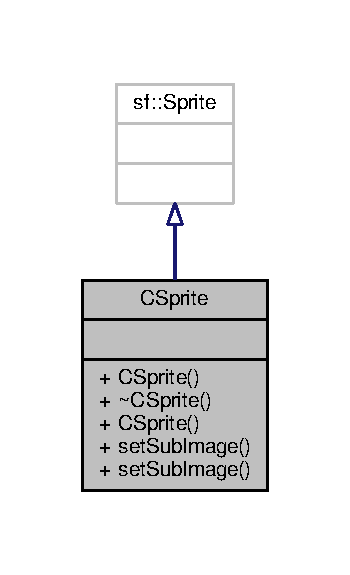
\includegraphics[width=168pt]{classCSprite__inherit__graph}
\end{center}
\end{figure}


Collaboration diagram for C\-Sprite\-:\nopagebreak
\begin{figure}[H]
\begin{center}
\leavevmode
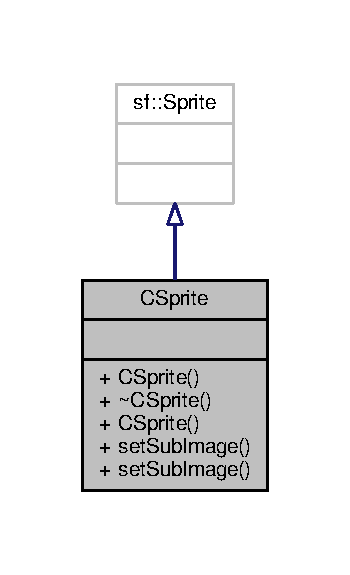
\includegraphics[width=168pt]{classCSprite__coll__graph}
\end{center}
\end{figure}
\subsection*{Public Member Functions}
\begin{DoxyCompactItemize}
\item 
\hyperlink{classCSprite_afdfe7ac25b872dbafd60e6329185b0c5}{C\-Sprite} (\hyperlink{classCTexture}{C\-Texture} $\ast$p\-Texture, const sf\-::\-Vector2$<$ int $>$ \&curr\-Sub)
\item 
\hyperlink{classCSprite_a274146d807d98947cff67621e783d31d}{$\sim$\-C\-Sprite} ()
\item 
\hyperlink{classCSprite_a7fa10fe45cf1683163671b7483ffc758}{C\-Sprite} (const \hyperlink{classCSprite}{C\-Sprite} \&other)
\item 
void \hyperlink{classCSprite_a2162a3b87f87eecf9e9b93fe4c573690}{set\-Sub\-Image} (int col, int row)
\begin{DoxyCompactList}\small\item\em sets the current sub image being rendered from the texture \end{DoxyCompactList}\item 
void \hyperlink{classCSprite_a6e46dd766754438ebdefadf3449540da}{set\-Sub\-Image} (const sf\-::\-Vector2$<$ int $>$ $\ast$new\-Sub)
\end{DoxyCompactItemize}


\subsection{Detailed Description}
Wrapper class for S\-F\-M\-L 2.\-1 Sprite. 

Definition at line 10 of file C\-Sprite.\-h.



\subsection{Constructor \& Destructor Documentation}
\hypertarget{classCSprite_afdfe7ac25b872dbafd60e6329185b0c5}{\index{C\-Sprite@{C\-Sprite}!C\-Sprite@{C\-Sprite}}
\index{C\-Sprite@{C\-Sprite}!CSprite@{C\-Sprite}}
\subsubsection[{C\-Sprite}]{\setlength{\rightskip}{0pt plus 5cm}C\-Sprite\-::\-C\-Sprite (
\begin{DoxyParamCaption}
\item[{{\bf C\-Texture} $\ast$}]{p\-Texture, }
\item[{const sf\-::\-Vector2$<$ int $>$ \&}]{curr\-Sub}
\end{DoxyParamCaption}
)}}\label{classCSprite_afdfe7ac25b872dbafd60e6329185b0c5}

\begin{DoxyParams}{Parameters}
{\em p\-Texture} & texture that this sprite will be rendering with \\
\hline
{\em curr\-Sub} & L\-E\-N\-G\-T\-H current sub-\/image being rendered \\
\hline
\end{DoxyParams}


Definition at line 6 of file C\-Sprite.\-cpp.

\hypertarget{classCSprite_a274146d807d98947cff67621e783d31d}{\index{C\-Sprite@{C\-Sprite}!$\sim$\-C\-Sprite@{$\sim$\-C\-Sprite}}
\index{$\sim$\-C\-Sprite@{$\sim$\-C\-Sprite}!CSprite@{C\-Sprite}}
\subsubsection[{$\sim$\-C\-Sprite}]{\setlength{\rightskip}{0pt plus 5cm}C\-Sprite\-::$\sim$\-C\-Sprite (
\begin{DoxyParamCaption}
{}
\end{DoxyParamCaption}
)}}\label{classCSprite_a274146d807d98947cff67621e783d31d}


Definition at line 19 of file C\-Sprite.\-cpp.

\hypertarget{classCSprite_a7fa10fe45cf1683163671b7483ffc758}{\index{C\-Sprite@{C\-Sprite}!C\-Sprite@{C\-Sprite}}
\index{C\-Sprite@{C\-Sprite}!CSprite@{C\-Sprite}}
\subsubsection[{C\-Sprite}]{\setlength{\rightskip}{0pt plus 5cm}C\-Sprite\-::\-C\-Sprite (
\begin{DoxyParamCaption}
\item[{const {\bf C\-Sprite} \&}]{other}
\end{DoxyParamCaption}
)}}\label{classCSprite_a7fa10fe45cf1683163671b7483ffc758}


Definition at line 24 of file C\-Sprite.\-cpp.



\subsection{Member Function Documentation}
\hypertarget{classCSprite_a2162a3b87f87eecf9e9b93fe4c573690}{\index{C\-Sprite@{C\-Sprite}!set\-Sub\-Image@{set\-Sub\-Image}}
\index{set\-Sub\-Image@{set\-Sub\-Image}!CSprite@{C\-Sprite}}
\subsubsection[{set\-Sub\-Image}]{\setlength{\rightskip}{0pt plus 5cm}void C\-Sprite\-::set\-Sub\-Image (
\begin{DoxyParamCaption}
\item[{int}]{col, }
\item[{int}]{row}
\end{DoxyParamCaption}
)}}\label{classCSprite_a2162a3b87f87eecf9e9b93fe4c573690}


sets the current sub image being rendered from the texture 



Definition at line 33 of file C\-Sprite.\-cpp.

\hypertarget{classCSprite_a6e46dd766754438ebdefadf3449540da}{\index{C\-Sprite@{C\-Sprite}!set\-Sub\-Image@{set\-Sub\-Image}}
\index{set\-Sub\-Image@{set\-Sub\-Image}!CSprite@{C\-Sprite}}
\subsubsection[{set\-Sub\-Image}]{\setlength{\rightskip}{0pt plus 5cm}void C\-Sprite\-::set\-Sub\-Image (
\begin{DoxyParamCaption}
\item[{const sf\-::\-Vector2$<$ int $>$ $\ast$}]{new\-Sub}
\end{DoxyParamCaption}
)}}\label{classCSprite_a6e46dd766754438ebdefadf3449540da}


Definition at line 46 of file C\-Sprite.\-cpp.



The documentation for this class was generated from the following files\-:\begin{DoxyCompactItemize}
\item 
/home/z\-Zelman/\-Dropbox/2\-D-\/\-Game\-Engine/src/\-Graphic/\hyperlink{CSprite_8h}{C\-Sprite.\-h}\item 
/home/z\-Zelman/\-Dropbox/2\-D-\/\-Game\-Engine/src/\-Graphic/\hyperlink{CSprite_8cpp}{C\-Sprite.\-cpp}\end{DoxyCompactItemize}

\hypertarget{classCTexture}{\section{C\-Texture Class Reference}
\label{classCTexture}\index{C\-Texture@{C\-Texture}}
}


Wrapper class for S\-F\-M\-L 2.\-1 Texture.  




{\ttfamily \#include $<$C\-Texture.\-h$>$}



Inheritance diagram for C\-Texture\-:\nopagebreak
\begin{figure}[H]
\begin{center}
\leavevmode
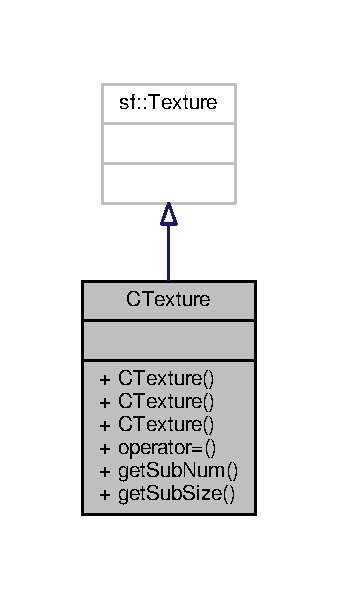
\includegraphics[width=162pt]{classCTexture__inherit__graph}
\end{center}
\end{figure}


Collaboration diagram for C\-Texture\-:\nopagebreak
\begin{figure}[H]
\begin{center}
\leavevmode
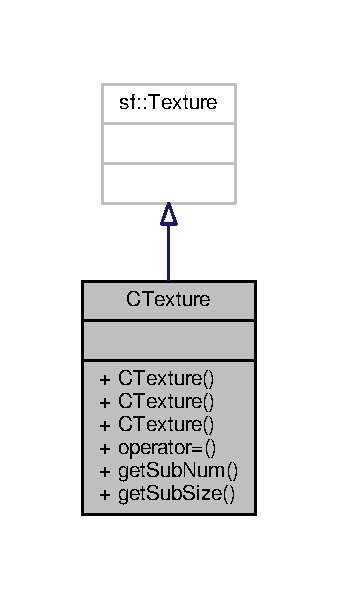
\includegraphics[width=162pt]{classCTexture__coll__graph}
\end{center}
\end{figure}
\subsection*{Public Member Functions}
\begin{DoxyCompactItemize}
\item 
\hyperlink{classCTexture_a4edabcc9e27ef0da135962c3490ec631}{C\-Texture} ()
\item 
\hyperlink{classCTexture_a03a03314b328783682d200443b561890}{C\-Texture} (std\-::string file\-Name, const sf\-::\-Vector2$<$ int $>$ \&sub\-Size, const sf\-::\-Vector2$<$ int $>$ \&sub\-Num)
\item 
\hyperlink{classCTexture_a2bb6709e0d63ccb6fb3219eb5528570f}{C\-Texture} (const \hyperlink{classCTexture}{C\-Texture} \&other)
\item 
\hyperlink{classCTexture}{C\-Texture} \& \hyperlink{classCTexture_ab4f29f7f73e347dfac33672e3b9a64c8}{operator=} (const \hyperlink{classCTexture}{C\-Texture} \&other)
\item 
const sf\-::\-Vector2$<$ int $>$ \& \hyperlink{classCTexture_a52a074211eaa812a91200f73f8387aca}{get\-Sub\-Num} () const 
\begin{DoxyCompactList}\small\item\em L\-E\-N\-G\-T\-H number of sub-\/section images on the full texture. \end{DoxyCompactList}\item 
const sf\-::\-Vector2$<$ int $>$ \& \hyperlink{classCTexture_a100f28379f113485d1e7574705ba977f}{get\-Sub\-Size} () const 
\begin{DoxyCompactList}\small\item\em L\-E\-N\-G\-T\-H of the sub-\/section image on the texture. \end{DoxyCompactList}\end{DoxyCompactItemize}


\subsection{Detailed Description}
Wrapper class for S\-F\-M\-L 2.\-1 Texture. 

Definition at line 16 of file C\-Texture.\-h.



\subsection{Constructor \& Destructor Documentation}
\hypertarget{classCTexture_a4edabcc9e27ef0da135962c3490ec631}{\index{C\-Texture@{C\-Texture}!C\-Texture@{C\-Texture}}
\index{C\-Texture@{C\-Texture}!CTexture@{C\-Texture}}
\subsubsection[{C\-Texture}]{\setlength{\rightskip}{0pt plus 5cm}C\-Texture\-::\-C\-Texture (
\begin{DoxyParamCaption}
{}
\end{DoxyParamCaption}
)}}\label{classCTexture_a4edabcc9e27ef0da135962c3490ec631}


Definition at line 13 of file C\-Texture.\-cpp.

\hypertarget{classCTexture_a03a03314b328783682d200443b561890}{\index{C\-Texture@{C\-Texture}!C\-Texture@{C\-Texture}}
\index{C\-Texture@{C\-Texture}!CTexture@{C\-Texture}}
\subsubsection[{C\-Texture}]{\setlength{\rightskip}{0pt plus 5cm}C\-Texture\-::\-C\-Texture (
\begin{DoxyParamCaption}
\item[{std\-::string}]{file\-Name, }
\item[{const sf\-::\-Vector2$<$ int $>$ \&}]{sub\-Size, }
\item[{const sf\-::\-Vector2$<$ int $>$ \&}]{sub\-Num}
\end{DoxyParamCaption}
)}}\label{classCTexture_a03a03314b328783682d200443b561890}

\begin{DoxyParams}{Parameters}
{\em file\-Name} & Relative full path to the texture image \\
\hline
{\em sub\-Size} & L\-E\-N\-G\-T\-H sub-\/image (x = width, y = height) \\
\hline
{\em sub\-Num} & L\-E\-N\-G\-T\-H number of sub images on the texture image \\
\hline
\end{DoxyParams}


Definition at line 19 of file C\-Texture.\-cpp.

\hypertarget{classCTexture_a2bb6709e0d63ccb6fb3219eb5528570f}{\index{C\-Texture@{C\-Texture}!C\-Texture@{C\-Texture}}
\index{C\-Texture@{C\-Texture}!CTexture@{C\-Texture}}
\subsubsection[{C\-Texture}]{\setlength{\rightskip}{0pt plus 5cm}C\-Texture\-::\-C\-Texture (
\begin{DoxyParamCaption}
\item[{const {\bf C\-Texture} \&}]{other}
\end{DoxyParamCaption}
)}}\label{classCTexture_a2bb6709e0d63ccb6fb3219eb5528570f}


Definition at line 31 of file C\-Texture.\-cpp.



\subsection{Member Function Documentation}
\hypertarget{classCTexture_a52a074211eaa812a91200f73f8387aca}{\index{C\-Texture@{C\-Texture}!get\-Sub\-Num@{get\-Sub\-Num}}
\index{get\-Sub\-Num@{get\-Sub\-Num}!CTexture@{C\-Texture}}
\subsubsection[{get\-Sub\-Num}]{\setlength{\rightskip}{0pt plus 5cm}const sf\-::\-Vector2$<$ int $>$ \& C\-Texture\-::get\-Sub\-Num (
\begin{DoxyParamCaption}
{}
\end{DoxyParamCaption}
) const}}\label{classCTexture_a52a074211eaa812a91200f73f8387aca}


L\-E\-N\-G\-T\-H number of sub-\/section images on the full texture. 

x = cols; y = rows 

Definition at line 56 of file C\-Texture.\-cpp.

\hypertarget{classCTexture_a100f28379f113485d1e7574705ba977f}{\index{C\-Texture@{C\-Texture}!get\-Sub\-Size@{get\-Sub\-Size}}
\index{get\-Sub\-Size@{get\-Sub\-Size}!CTexture@{C\-Texture}}
\subsubsection[{get\-Sub\-Size}]{\setlength{\rightskip}{0pt plus 5cm}const sf\-::\-Vector2$<$ int $>$ \& C\-Texture\-::get\-Sub\-Size (
\begin{DoxyParamCaption}
{}
\end{DoxyParamCaption}
) const}}\label{classCTexture_a100f28379f113485d1e7574705ba977f}


L\-E\-N\-G\-T\-H of the sub-\/section image on the texture. 

x = width; y = height 

Definition at line 62 of file C\-Texture.\-cpp.

\hypertarget{classCTexture_ab4f29f7f73e347dfac33672e3b9a64c8}{\index{C\-Texture@{C\-Texture}!operator=@{operator=}}
\index{operator=@{operator=}!CTexture@{C\-Texture}}
\subsubsection[{operator=}]{\setlength{\rightskip}{0pt plus 5cm}{\bf C\-Texture} \& C\-Texture\-::operator= (
\begin{DoxyParamCaption}
\item[{const {\bf C\-Texture} \&}]{other}
\end{DoxyParamCaption}
)}}\label{classCTexture_ab4f29f7f73e347dfac33672e3b9a64c8}


Definition at line 39 of file C\-Texture.\-cpp.



The documentation for this class was generated from the following files\-:\begin{DoxyCompactItemize}
\item 
/home/z\-Zelman/\-Dropbox/\-Marshmallow-\/\-Duels/src/\-Headers/\hyperlink{CTexture_8h}{C\-Texture.\-h}\item 
/home/z\-Zelman/\-Dropbox/\-Marshmallow-\/\-Duels/src/\-Graphics/\hyperlink{CTexture_8cpp}{C\-Texture.\-cpp}\end{DoxyCompactItemize}

\hypertarget{classGameElement__movable}{\section{Game\-Element\-\_\-movable Class Reference}
\label{classGameElement__movable}\index{Game\-Element\-\_\-movable@{Game\-Element\-\_\-movable}}
}


{\ttfamily \#include $<$Game\-Element\-\_\-movable.\-h$>$}



Inheritance diagram for Game\-Element\-\_\-movable\-:\nopagebreak
\begin{figure}[H]
\begin{center}
\leavevmode
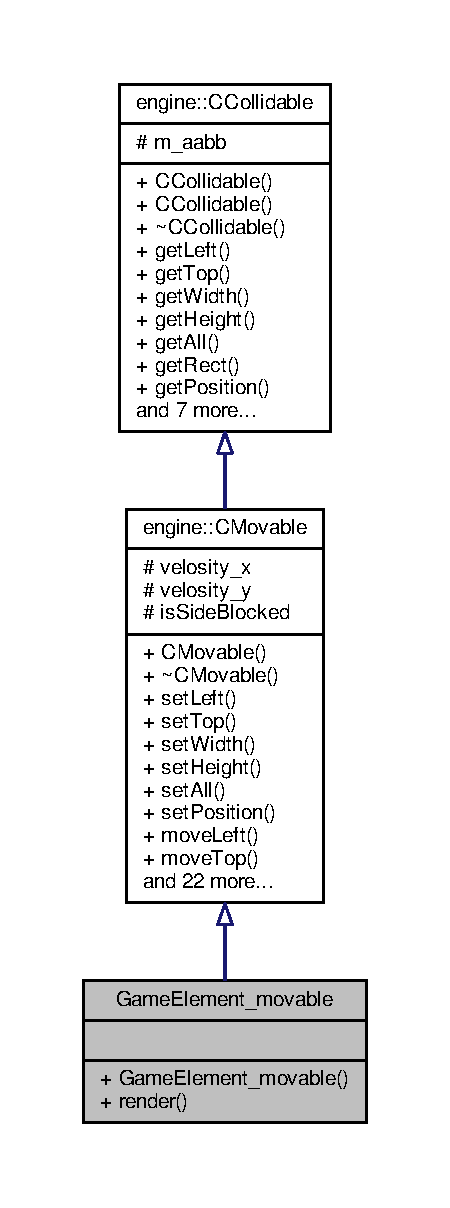
\includegraphics[height=550pt]{classGameElement__movable__inherit__graph}
\end{center}
\end{figure}


Collaboration diagram for Game\-Element\-\_\-movable\-:\nopagebreak
\begin{figure}[H]
\begin{center}
\leavevmode
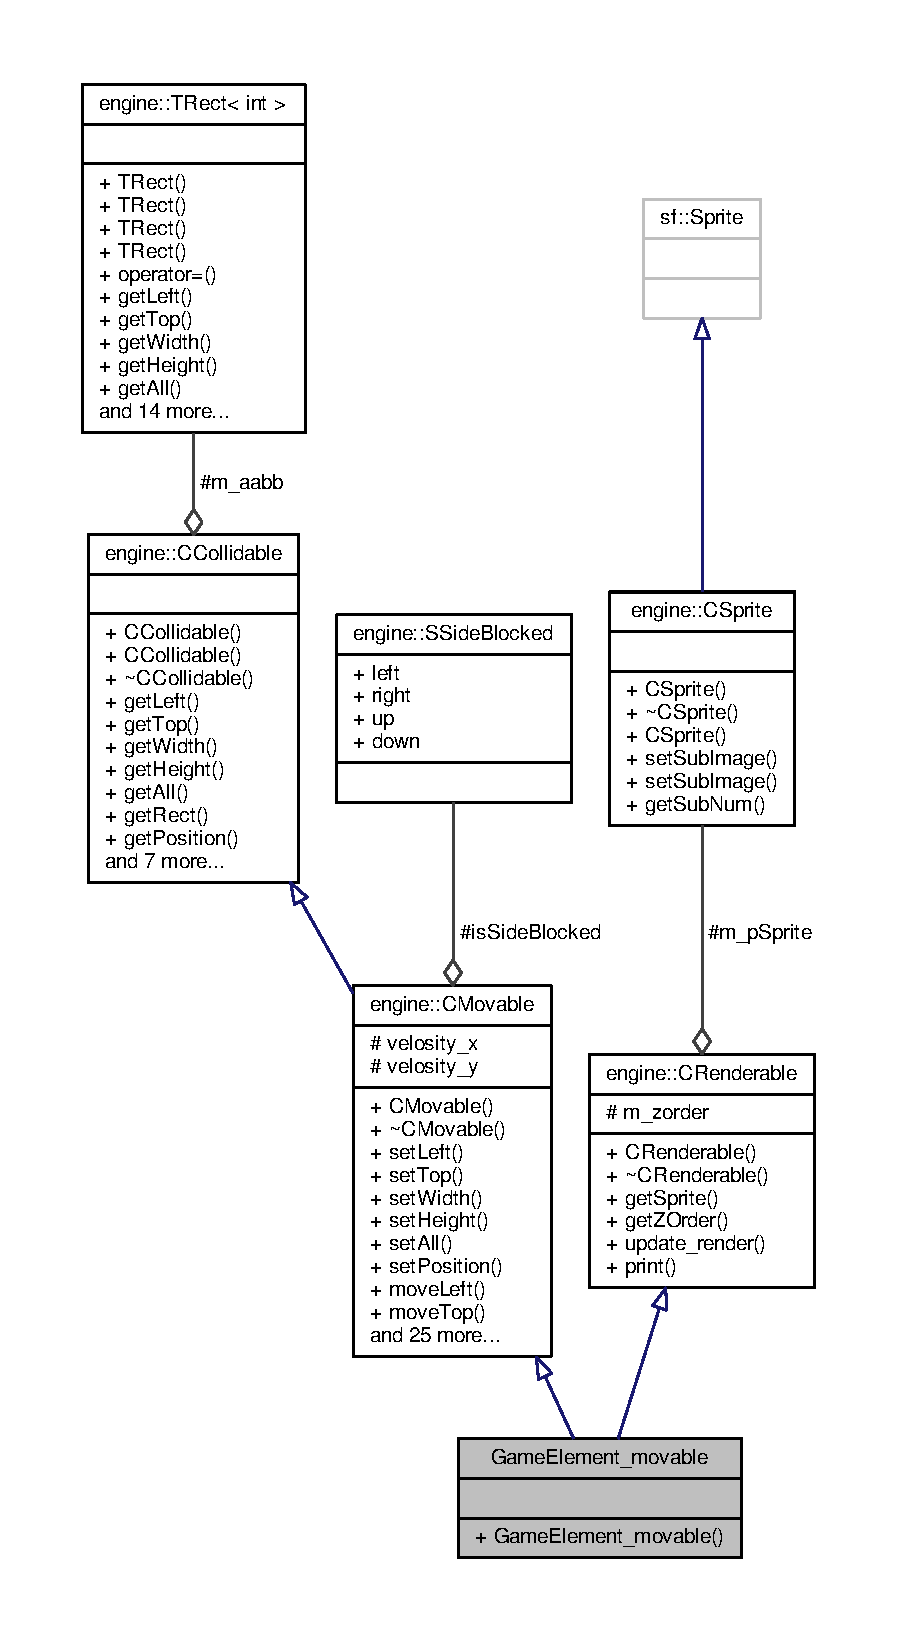
\includegraphics[height=550pt]{classGameElement__movable__coll__graph}
\end{center}
\end{figure}
\subsection*{Public Member Functions}
\begin{DoxyCompactItemize}
\item 
\hyperlink{classGameElement__movable_ac9009600530046f90e75ebcea411d907}{Game\-Element\-\_\-movable} (\hyperlink{classCSprite}{C\-Sprite} $\ast$sprite, sf\-::\-Render\-Window $\ast$window)
\item 
void \hyperlink{classGameElement__movable_a503e47a89c65d149529a3af6dc1064a1}{render} ()
\end{DoxyCompactItemize}
\subsection*{Additional Inherited Members}


\subsection{Detailed Description}


Definition at line 8 of file Game\-Element\-\_\-movable.\-h.



\subsection{Constructor \& Destructor Documentation}
\hypertarget{classGameElement__movable_ac9009600530046f90e75ebcea411d907}{\index{Game\-Element\-\_\-movable@{Game\-Element\-\_\-movable}!Game\-Element\-\_\-movable@{Game\-Element\-\_\-movable}}
\index{Game\-Element\-\_\-movable@{Game\-Element\-\_\-movable}!GameElement_movable@{Game\-Element\-\_\-movable}}
\subsubsection[{Game\-Element\-\_\-movable}]{\setlength{\rightskip}{0pt plus 5cm}Game\-Element\-\_\-movable\-::\-Game\-Element\-\_\-movable (
\begin{DoxyParamCaption}
\item[{{\bf C\-Sprite} $\ast$}]{sprite, }
\item[{sf\-::\-Render\-Window $\ast$}]{window}
\end{DoxyParamCaption}
)}}\label{classGameElement__movable_ac9009600530046f90e75ebcea411d907}


Definition at line 3 of file Game\-Element\-\_\-movable.\-cpp.



\subsection{Member Function Documentation}
\hypertarget{classGameElement__movable_a503e47a89c65d149529a3af6dc1064a1}{\index{Game\-Element\-\_\-movable@{Game\-Element\-\_\-movable}!render@{render}}
\index{render@{render}!GameElement_movable@{Game\-Element\-\_\-movable}}
\subsubsection[{render}]{\setlength{\rightskip}{0pt plus 5cm}void Game\-Element\-\_\-movable\-::render (
\begin{DoxyParamCaption}
{}
\end{DoxyParamCaption}
)}}\label{classGameElement__movable_a503e47a89c65d149529a3af6dc1064a1}


Definition at line 10 of file Game\-Element\-\_\-movable.\-cpp.



The documentation for this class was generated from the following files\-:\begin{DoxyCompactItemize}
\item 
/home/z\-Zelman/\-Dropbox/2\-D-\/\-Game\-Engine/src/\hyperlink{GameElement__movable_8h}{Game\-Element\-\_\-movable.\-h}\item 
/home/z\-Zelman/\-Dropbox/2\-D-\/\-Game\-Engine/src/\hyperlink{GameElement__movable_8cpp}{Game\-Element\-\_\-movable.\-cpp}\end{DoxyCompactItemize}

\hypertarget{classGameElement__static}{\section{Game\-Element\-\_\-static Class Reference}
\label{classGameElement__static}\index{Game\-Element\-\_\-static@{Game\-Element\-\_\-static}}
}


{\ttfamily \#include $<$Game\-Element\-\_\-static.\-h$>$}



Inheritance diagram for Game\-Element\-\_\-static\-:\nopagebreak
\begin{figure}[H]
\begin{center}
\leavevmode
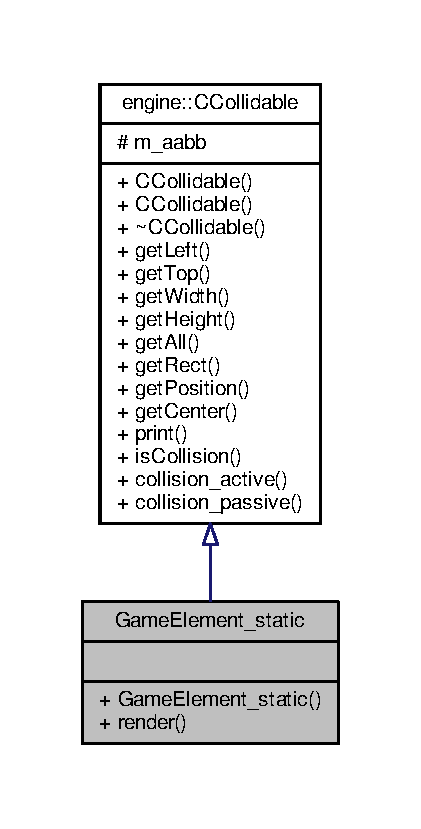
\includegraphics[width=202pt]{classGameElement__static__inherit__graph}
\end{center}
\end{figure}


Collaboration diagram for Game\-Element\-\_\-static\-:\nopagebreak
\begin{figure}[H]
\begin{center}
\leavevmode
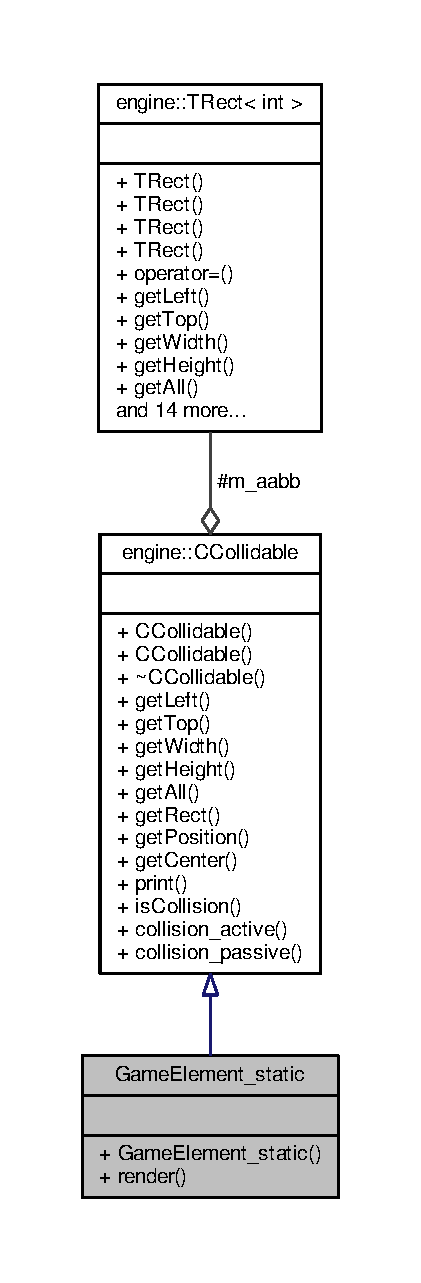
\includegraphics[height=550pt]{classGameElement__static__coll__graph}
\end{center}
\end{figure}
\subsection*{Public Member Functions}
\begin{DoxyCompactItemize}
\item 
\hyperlink{classGameElement__static_a1eb5f044f28720fe41fd57851a1ee168}{Game\-Element\-\_\-static} (\hyperlink{classengine_1_1CSprite}{engine\-::\-C\-Sprite} $\ast$sprite, sf\-::\-Render\-Window $\ast$window)
\item 
void \hyperlink{classGameElement__static_aa5fe0d840d4f306ac38c8e55cfc7616f}{render} ()
\end{DoxyCompactItemize}
\subsection*{Additional Inherited Members}


\subsection{Detailed Description}


Definition at line 6 of file Game\-Element\-\_\-static.\-h.



\subsection{Constructor \& Destructor Documentation}
\hypertarget{classGameElement__static_a1eb5f044f28720fe41fd57851a1ee168}{\index{Game\-Element\-\_\-static@{Game\-Element\-\_\-static}!Game\-Element\-\_\-static@{Game\-Element\-\_\-static}}
\index{Game\-Element\-\_\-static@{Game\-Element\-\_\-static}!GameElement_static@{Game\-Element\-\_\-static}}
\subsubsection[{Game\-Element\-\_\-static}]{\setlength{\rightskip}{0pt plus 5cm}Game\-Element\-\_\-static\-::\-Game\-Element\-\_\-static (
\begin{DoxyParamCaption}
\item[{{\bf engine\-::\-C\-Sprite} $\ast$}]{sprite, }
\item[{sf\-::\-Render\-Window $\ast$}]{window}
\end{DoxyParamCaption}
)}}\label{classGameElement__static_a1eb5f044f28720fe41fd57851a1ee168}


Definition at line 3 of file Game\-Element\-\_\-static.\-cpp.



\subsection{Member Function Documentation}
\hypertarget{classGameElement__static_aa5fe0d840d4f306ac38c8e55cfc7616f}{\index{Game\-Element\-\_\-static@{Game\-Element\-\_\-static}!render@{render}}
\index{render@{render}!GameElement_static@{Game\-Element\-\_\-static}}
\subsubsection[{render}]{\setlength{\rightskip}{0pt plus 5cm}void Game\-Element\-\_\-static\-::render (
\begin{DoxyParamCaption}
{}
\end{DoxyParamCaption}
)}}\label{classGameElement__static_aa5fe0d840d4f306ac38c8e55cfc7616f}


Definition at line 11 of file Game\-Element\-\_\-static.\-cpp.



The documentation for this class was generated from the following files\-:\begin{DoxyCompactItemize}
\item 
/home/z\-Zelman/\-Dropbox/2\-D-\/\-Game\-Engine/src/\hyperlink{GameElement__static_8h}{Game\-Element\-\_\-static.\-h}\item 
/home/z\-Zelman/\-Dropbox/2\-D-\/\-Game\-Engine/src/\hyperlink{GameElement__static_8cpp}{Game\-Element\-\_\-static.\-cpp}\end{DoxyCompactItemize}

\hypertarget{classengine_1_1PhysicsEngine}{\section{engine\-:\-:Physics\-Engine Class Reference}
\label{classengine_1_1PhysicsEngine}\index{engine\-::\-Physics\-Engine@{engine\-::\-Physics\-Engine}}
}


{\ttfamily \#include $<$Physics\-Engine.\-h$>$}



Collaboration diagram for engine\-:\-:Physics\-Engine\-:
\nopagebreak
\begin{figure}[H]
\begin{center}
\leavevmode
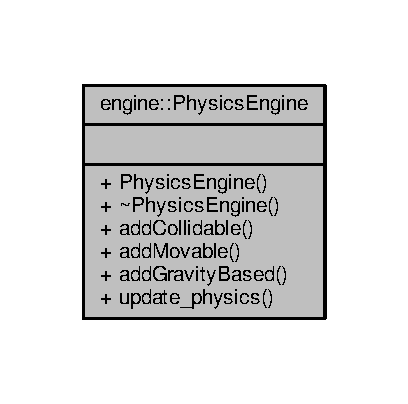
\includegraphics[width=196pt]{classengine_1_1PhysicsEngine__coll__graph}
\end{center}
\end{figure}
\subsection*{Public Member Functions}
\begin{DoxyCompactItemize}
\item 
\hyperlink{classengine_1_1PhysicsEngine_a14c98b9b2eae12bff267b99df27ac9fc}{Physics\-Engine} ()
\item 
virtual \hyperlink{classengine_1_1PhysicsEngine_a7b708ba5517fdd9cc95c977dde7ff4ab}{$\sim$\-Physics\-Engine} ()
\item 
void \hyperlink{classengine_1_1PhysicsEngine_a609b1b5b818d7865c9b20abfe07e26e8}{add\-Collidable} (\hyperlink{classengine_1_1CCollidable}{C\-Collidable} $\ast$c)
\item 
void \hyperlink{classengine_1_1PhysicsEngine_a32690f48a5df0b98c5f326c0b11414ba}{add\-Movable} (\hyperlink{classengine_1_1CMovable}{C\-Movable} $\ast$m)
\item 
void \hyperlink{classengine_1_1PhysicsEngine_a468ef9599ccd80e7e5c170d741ab1d21}{update} ()
\end{DoxyCompactItemize}


\subsection{Detailed Description}


Definition at line 12 of file Physics\-Engine.\-h.



\subsection{Constructor \& Destructor Documentation}
\hypertarget{classengine_1_1PhysicsEngine_a14c98b9b2eae12bff267b99df27ac9fc}{\index{engine\-::\-Physics\-Engine@{engine\-::\-Physics\-Engine}!Physics\-Engine@{Physics\-Engine}}
\index{Physics\-Engine@{Physics\-Engine}!engine::PhysicsEngine@{engine\-::\-Physics\-Engine}}
\subsubsection[{Physics\-Engine}]{\setlength{\rightskip}{0pt plus 5cm}engine\-::\-Physics\-Engine\-::\-Physics\-Engine (
\begin{DoxyParamCaption}
{}
\end{DoxyParamCaption}
)}}\label{classengine_1_1PhysicsEngine_a14c98b9b2eae12bff267b99df27ac9fc}


Definition at line 9 of file Physics\-Engine.\-cpp.

\hypertarget{classengine_1_1PhysicsEngine_a7b708ba5517fdd9cc95c977dde7ff4ab}{\index{engine\-::\-Physics\-Engine@{engine\-::\-Physics\-Engine}!$\sim$\-Physics\-Engine@{$\sim$\-Physics\-Engine}}
\index{$\sim$\-Physics\-Engine@{$\sim$\-Physics\-Engine}!engine::PhysicsEngine@{engine\-::\-Physics\-Engine}}
\subsubsection[{$\sim$\-Physics\-Engine}]{\setlength{\rightskip}{0pt plus 5cm}engine\-::\-Physics\-Engine\-::$\sim$\-Physics\-Engine (
\begin{DoxyParamCaption}
{}
\end{DoxyParamCaption}
)\hspace{0.3cm}{\ttfamily [virtual]}}}\label{classengine_1_1PhysicsEngine_a7b708ba5517fdd9cc95c977dde7ff4ab}


Definition at line 14 of file Physics\-Engine.\-cpp.



\subsection{Member Function Documentation}
\hypertarget{classengine_1_1PhysicsEngine_a609b1b5b818d7865c9b20abfe07e26e8}{\index{engine\-::\-Physics\-Engine@{engine\-::\-Physics\-Engine}!add\-Collidable@{add\-Collidable}}
\index{add\-Collidable@{add\-Collidable}!engine::PhysicsEngine@{engine\-::\-Physics\-Engine}}
\subsubsection[{add\-Collidable}]{\setlength{\rightskip}{0pt plus 5cm}void engine\-::\-Physics\-Engine\-::add\-Collidable (
\begin{DoxyParamCaption}
\item[{{\bf C\-Collidable} $\ast$}]{c}
\end{DoxyParamCaption}
)}}\label{classengine_1_1PhysicsEngine_a609b1b5b818d7865c9b20abfe07e26e8}


Definition at line 19 of file Physics\-Engine.\-cpp.

\hypertarget{classengine_1_1PhysicsEngine_a32690f48a5df0b98c5f326c0b11414ba}{\index{engine\-::\-Physics\-Engine@{engine\-::\-Physics\-Engine}!add\-Movable@{add\-Movable}}
\index{add\-Movable@{add\-Movable}!engine::PhysicsEngine@{engine\-::\-Physics\-Engine}}
\subsubsection[{add\-Movable}]{\setlength{\rightskip}{0pt plus 5cm}void engine\-::\-Physics\-Engine\-::add\-Movable (
\begin{DoxyParamCaption}
\item[{{\bf C\-Movable} $\ast$}]{m}
\end{DoxyParamCaption}
)}}\label{classengine_1_1PhysicsEngine_a32690f48a5df0b98c5f326c0b11414ba}


Definition at line 25 of file Physics\-Engine.\-cpp.

\hypertarget{classengine_1_1PhysicsEngine_a468ef9599ccd80e7e5c170d741ab1d21}{\index{engine\-::\-Physics\-Engine@{engine\-::\-Physics\-Engine}!update@{update}}
\index{update@{update}!engine::PhysicsEngine@{engine\-::\-Physics\-Engine}}
\subsubsection[{update}]{\setlength{\rightskip}{0pt plus 5cm}void engine\-::\-Physics\-Engine\-::update (
\begin{DoxyParamCaption}
{}
\end{DoxyParamCaption}
)}}\label{classengine_1_1PhysicsEngine_a468ef9599ccd80e7e5c170d741ab1d21}


Definition at line 31 of file Physics\-Engine.\-cpp.



The documentation for this class was generated from the following files\-:\begin{DoxyCompactItemize}
\item 
/home/z\-Zelman/\-Dropbox/2\-D-\/\-Game\-Engine/src/\-Physics/\hyperlink{PhysicsEngine_8h}{Physics\-Engine.\-h}\item 
/home/z\-Zelman/\-Dropbox/2\-D-\/\-Game\-Engine/src/\-Physics/\hyperlink{PhysicsEngine_8cpp}{Physics\-Engine.\-cpp}\end{DoxyCompactItemize}

\hypertarget{structengine_1_1SSideBlocked}{\section{engine\-:\-:S\-Side\-Blocked Struct Reference}
\label{structengine_1_1SSideBlocked}\index{engine\-::\-S\-Side\-Blocked@{engine\-::\-S\-Side\-Blocked}}
}


A plane-\/old-\/data-\/structure to tell whether the directions are \char`\"{}physically\char`\"{} blocked for movement.  




{\ttfamily \#include $<$C\-Movable.\-h$>$}



Collaboration diagram for engine\-:\-:S\-Side\-Blocked\-:\nopagebreak
\begin{figure}[H]
\begin{center}
\leavevmode
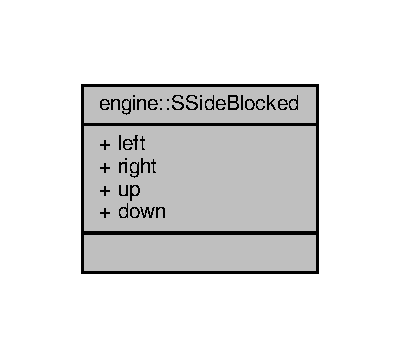
\includegraphics[width=192pt]{structengine_1_1SSideBlocked__coll__graph}
\end{center}
\end{figure}
\subsection*{Public Attributes}
\begin{DoxyCompactItemize}
\item 
bool \hyperlink{structengine_1_1SSideBlocked_aab2ebe596bade5dd2111290ff4171268}{left}
\item 
bool \hyperlink{structengine_1_1SSideBlocked_af6f555a50cd295e753bc57ba1fe98b7b}{right}
\item 
bool \hyperlink{structengine_1_1SSideBlocked_a62f8b294229bf0f52bc01ffcc9086202}{up}
\item 
bool \hyperlink{structengine_1_1SSideBlocked_ab0a5ec3de4a3a1f71eb8c28dcaa113ec}{down}
\end{DoxyCompactItemize}


\subsection{Detailed Description}
A plane-\/old-\/data-\/structure to tell whether the directions are \char`\"{}physically\char`\"{} blocked for movement. 

Definition at line 13 of file C\-Movable.\-h.



\subsection{Member Data Documentation}
\hypertarget{structengine_1_1SSideBlocked_ab0a5ec3de4a3a1f71eb8c28dcaa113ec}{\index{engine\-::\-S\-Side\-Blocked@{engine\-::\-S\-Side\-Blocked}!down@{down}}
\index{down@{down}!engine::SSideBlocked@{engine\-::\-S\-Side\-Blocked}}
\subsubsection[{down}]{\setlength{\rightskip}{0pt plus 5cm}bool engine\-::\-S\-Side\-Blocked\-::down}}\label{structengine_1_1SSideBlocked_ab0a5ec3de4a3a1f71eb8c28dcaa113ec}


Definition at line 15 of file C\-Movable.\-h.

\hypertarget{structengine_1_1SSideBlocked_aab2ebe596bade5dd2111290ff4171268}{\index{engine\-::\-S\-Side\-Blocked@{engine\-::\-S\-Side\-Blocked}!left@{left}}
\index{left@{left}!engine::SSideBlocked@{engine\-::\-S\-Side\-Blocked}}
\subsubsection[{left}]{\setlength{\rightskip}{0pt plus 5cm}bool engine\-::\-S\-Side\-Blocked\-::left}}\label{structengine_1_1SSideBlocked_aab2ebe596bade5dd2111290ff4171268}


Definition at line 15 of file C\-Movable.\-h.

\hypertarget{structengine_1_1SSideBlocked_af6f555a50cd295e753bc57ba1fe98b7b}{\index{engine\-::\-S\-Side\-Blocked@{engine\-::\-S\-Side\-Blocked}!right@{right}}
\index{right@{right}!engine::SSideBlocked@{engine\-::\-S\-Side\-Blocked}}
\subsubsection[{right}]{\setlength{\rightskip}{0pt plus 5cm}bool engine\-::\-S\-Side\-Blocked\-::right}}\label{structengine_1_1SSideBlocked_af6f555a50cd295e753bc57ba1fe98b7b}


Definition at line 15 of file C\-Movable.\-h.

\hypertarget{structengine_1_1SSideBlocked_a62f8b294229bf0f52bc01ffcc9086202}{\index{engine\-::\-S\-Side\-Blocked@{engine\-::\-S\-Side\-Blocked}!up@{up}}
\index{up@{up}!engine::SSideBlocked@{engine\-::\-S\-Side\-Blocked}}
\subsubsection[{up}]{\setlength{\rightskip}{0pt plus 5cm}bool engine\-::\-S\-Side\-Blocked\-::up}}\label{structengine_1_1SSideBlocked_a62f8b294229bf0f52bc01ffcc9086202}


Definition at line 15 of file C\-Movable.\-h.



The documentation for this struct was generated from the following file\-:\begin{DoxyCompactItemize}
\item 
/home/z\-Zelman/\-Dropbox/2\-D-\/\-Game\-Engine/src/\-Physics/\hyperlink{CMovable_8h}{C\-Movable.\-h}\end{DoxyCompactItemize}

\hypertarget{classengine_1_1TRect}{\section{engine\-:\-:T\-Rect$<$ T $>$ Class Template Reference}
\label{classengine_1_1TRect}\index{engine\-::\-T\-Rect$<$ T $>$@{engine\-::\-T\-Rect$<$ T $>$}}
}


A template class for a Rectangle that the physics engine uses.  




{\ttfamily \#include $<$T\-Rect.\-h$>$}



Collaboration diagram for engine\-:\-:T\-Rect$<$ T $>$\-:
\nopagebreak
\begin{figure}[H]
\begin{center}
\leavevmode
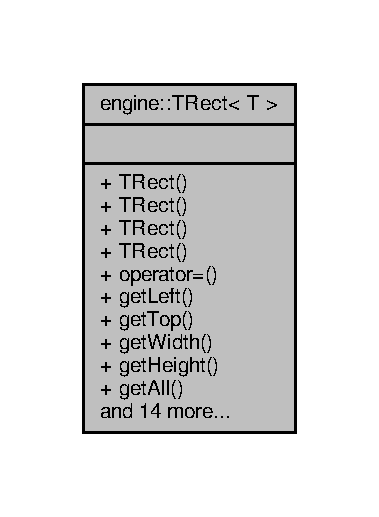
\includegraphics[width=182pt]{classengine_1_1TRect__coll__graph}
\end{center}
\end{figure}
\subsection*{Public Member Functions}
\begin{DoxyCompactItemize}
\item 
\hyperlink{classengine_1_1TRect_a6ac360fa89c33540e1aacf0217bcbff7}{T\-Rect} ()
\begin{DoxyCompactList}\small\item\em Sets member variables at (0, 0, 100, 100) \end{DoxyCompactList}\item 
\hyperlink{classengine_1_1TRect_af74e4c9b5d570438a25c8b92d9b946d4}{T\-Rect} (T left, T top, T width, T height)
\begin{DoxyCompactList}\small\item\em Creates a rect with given values. \end{DoxyCompactList}\item 
\hyperlink{classengine_1_1TRect_a3d400a91242673bf38496a724543f98a}{T\-Rect} (\hyperlink{classCSprite}{C\-Sprite} $\ast$sprite)
\begin{DoxyCompactList}\small\item\em Copies the dominations from the given \hyperlink{classCSprite}{C\-Sprite} into this Rect D\-O\-E\-S N\-O\-T keep the sprite around. \end{DoxyCompactList}\item 
\hyperlink{classengine_1_1TRect_a4a4706672995ba4fabd6be900b58ce1f}{T\-Rect} (const \hyperlink{classengine_1_1TRect}{T\-Rect}$<$ T $>$ \&other)
\item 
\hyperlink{classengine_1_1TRect}{T\-Rect} \& \hyperlink{classengine_1_1TRect_a4ccd990e5432e94ca3b8280cf9c73e0e}{operator=} (const \hyperlink{classengine_1_1TRect}{T\-Rect}$<$ T $>$ \&other)
\item 
T \hyperlink{classengine_1_1TRect_aa813022ee910757ce429aae829023d53}{get\-Left} () const 
\item 
T \hyperlink{classengine_1_1TRect_ae622bc0564f8d15556f32844be907adf}{get\-Top} () const 
\item 
T \hyperlink{classengine_1_1TRect_afe9eb87a07784381d0172cebac589ed0}{get\-Width} () const 
\item 
T \hyperlink{classengine_1_1TRect_ac377947f57b80de2c3c94d21e66e97cf}{get\-Height} () const 
\item 
void \hyperlink{classengine_1_1TRect_a73a225ba48ce45915087fe7a94c2ab1f}{get\-All} (T \&left, T \&top, T \&width, T \&height) const 
\item 
void \hyperlink{classengine_1_1TRect_a9b563983bf2839c51db741cdd0b90058}{get\-Rect} (\hyperlink{classengine_1_1TRect}{T\-Rect}$<$ int $>$ $\ast$rect) const 
\item 
void \hyperlink{classengine_1_1TRect_a6ec7dc08118c6012d17327ca8934d2e0}{get\-Position} (T \&left, T \&top) const 
\item 
void \hyperlink{classengine_1_1TRect_a34c390356af6890b4d4a5ef3d19694cf}{get\-Center} (T \&x, T \&y) const 
\item 
void \hyperlink{classengine_1_1TRect_aa0f1c4e8042c553fb3a9ad0805a58bb3}{set\-Left} (T left)
\item 
void \hyperlink{classengine_1_1TRect_aca4664e0e6d9736ffbc48663f9e8cd3f}{set\-Top} (T top)
\item 
void \hyperlink{classengine_1_1TRect_aad5a2530169d7953634fea4515381c37}{set\-Width} (T width)
\item 
void \hyperlink{classengine_1_1TRect_ae29fe9d2401f49e84f6c070ef60e9d7b}{set\-Height} (T height)
\item 
void \hyperlink{classengine_1_1TRect_ae10bacc96b54c45b2722e51b045ae3fe}{set\-All} (T left, T top, T width, T height)
\item 
void \hyperlink{classengine_1_1TRect_a41cce51fffc829c4d3e5dc40f605cb9e}{set\-All} (\hyperlink{classCSprite}{C\-Sprite} $\ast$sprite)
\begin{DoxyCompactList}\small\item\em Copies the dominations from the given \hyperlink{classCSprite}{C\-Sprite} into this Rect D\-O\-E\-S N\-O\-T keep the sprite around. \end{DoxyCompactList}\item 
void \hyperlink{classengine_1_1TRect_ad7bdff230a7152e3d8ed3934046bed7c}{set\-Position} (T left, T top)
\item 
void \hyperlink{classengine_1_1TRect_a0699fb896f494a85e24abe32066ae5d9}{move\-Left} (T d\-\_\-left)
\item 
void \hyperlink{classengine_1_1TRect_a7e65ccfa166f4d7690d87e6985182379}{move\-Top} (T d\-\_\-top)
\item 
void \hyperlink{classengine_1_1TRect_a2650390138117e0ad1eecc8124735bd9}{move\-Position} (T d\-\_\-left, T d\-\_\-top)
\end{DoxyCompactItemize}


\subsection{Detailed Description}
\subsubsection*{template$<$class T$>$class engine\-::\-T\-Rect$<$ T $>$}

A template class for a Rectangle that the physics engine uses. 

Can be used to represent an Axis Aligned Bounding Box (A\-A\-B\-B). 

Definition at line 19 of file T\-Rect.\-h.



\subsection{Constructor \& Destructor Documentation}
\hypertarget{classengine_1_1TRect_a6ac360fa89c33540e1aacf0217bcbff7}{\index{engine\-::\-T\-Rect@{engine\-::\-T\-Rect}!T\-Rect@{T\-Rect}}
\index{T\-Rect@{T\-Rect}!engine::TRect@{engine\-::\-T\-Rect}}
\subsubsection[{T\-Rect}]{\setlength{\rightskip}{0pt plus 5cm}template$<$class T $>$ {\bf engine\-::\-T\-Rect}$<$ T $>$\-::{\bf T\-Rect} (
\begin{DoxyParamCaption}
{}
\end{DoxyParamCaption}
)\hspace{0.3cm}{\ttfamily [inline]}}}\label{classengine_1_1TRect_a6ac360fa89c33540e1aacf0217bcbff7}


Sets member variables at (0, 0, 100, 100) 



Definition at line 77 of file T\-Rect.\-h.

\hypertarget{classengine_1_1TRect_af74e4c9b5d570438a25c8b92d9b946d4}{\index{engine\-::\-T\-Rect@{engine\-::\-T\-Rect}!T\-Rect@{T\-Rect}}
\index{T\-Rect@{T\-Rect}!engine::TRect@{engine\-::\-T\-Rect}}
\subsubsection[{T\-Rect}]{\setlength{\rightskip}{0pt plus 5cm}template$<$class T$>$ {\bf engine\-::\-T\-Rect}$<$ T $>$\-::{\bf T\-Rect} (
\begin{DoxyParamCaption}
\item[{T}]{left, }
\item[{T}]{top, }
\item[{T}]{width, }
\item[{T}]{height}
\end{DoxyParamCaption}
)\hspace{0.3cm}{\ttfamily [inline]}}}\label{classengine_1_1TRect_af74e4c9b5d570438a25c8b92d9b946d4}


Creates a rect with given values. 



Definition at line 83 of file T\-Rect.\-h.

\hypertarget{classengine_1_1TRect_a3d400a91242673bf38496a724543f98a}{\index{engine\-::\-T\-Rect@{engine\-::\-T\-Rect}!T\-Rect@{T\-Rect}}
\index{T\-Rect@{T\-Rect}!engine::TRect@{engine\-::\-T\-Rect}}
\subsubsection[{T\-Rect}]{\setlength{\rightskip}{0pt plus 5cm}template$<$class T$>$ {\bf engine\-::\-T\-Rect}$<$ T $>$\-::{\bf T\-Rect} (
\begin{DoxyParamCaption}
\item[{{\bf C\-Sprite} $\ast$}]{sprite}
\end{DoxyParamCaption}
)\hspace{0.3cm}{\ttfamily [inline]}}}\label{classengine_1_1TRect_a3d400a91242673bf38496a724543f98a}


Copies the dominations from the given \hyperlink{classCSprite}{C\-Sprite} into this Rect D\-O\-E\-S N\-O\-T keep the sprite around. 



Definition at line 89 of file T\-Rect.\-h.

\hypertarget{classengine_1_1TRect_a4a4706672995ba4fabd6be900b58ce1f}{\index{engine\-::\-T\-Rect@{engine\-::\-T\-Rect}!T\-Rect@{T\-Rect}}
\index{T\-Rect@{T\-Rect}!engine::TRect@{engine\-::\-T\-Rect}}
\subsubsection[{T\-Rect}]{\setlength{\rightskip}{0pt plus 5cm}template$<$class T$>$ {\bf engine\-::\-T\-Rect}$<$ T $>$\-::{\bf T\-Rect} (
\begin{DoxyParamCaption}
\item[{const {\bf T\-Rect}$<$ T $>$ \&}]{other}
\end{DoxyParamCaption}
)\hspace{0.3cm}{\ttfamily [inline]}}}\label{classengine_1_1TRect_a4a4706672995ba4fabd6be900b58ce1f}


Definition at line 98 of file T\-Rect.\-h.



\subsection{Member Function Documentation}
\hypertarget{classengine_1_1TRect_a73a225ba48ce45915087fe7a94c2ab1f}{\index{engine\-::\-T\-Rect@{engine\-::\-T\-Rect}!get\-All@{get\-All}}
\index{get\-All@{get\-All}!engine::TRect@{engine\-::\-T\-Rect}}
\subsubsection[{get\-All}]{\setlength{\rightskip}{0pt plus 5cm}template$<$class T$>$ void {\bf engine\-::\-T\-Rect}$<$ T $>$\-::get\-All (
\begin{DoxyParamCaption}
\item[{T \&}]{left, }
\item[{T \&}]{top, }
\item[{T \&}]{width, }
\item[{T \&}]{height}
\end{DoxyParamCaption}
) const\hspace{0.3cm}{\ttfamily [inline]}}}\label{classengine_1_1TRect_a73a225ba48ce45915087fe7a94c2ab1f}


Definition at line 143 of file T\-Rect.\-h.

\hypertarget{classengine_1_1TRect_a34c390356af6890b4d4a5ef3d19694cf}{\index{engine\-::\-T\-Rect@{engine\-::\-T\-Rect}!get\-Center@{get\-Center}}
\index{get\-Center@{get\-Center}!engine::TRect@{engine\-::\-T\-Rect}}
\subsubsection[{get\-Center}]{\setlength{\rightskip}{0pt plus 5cm}template$<$class T$>$ void {\bf engine\-::\-T\-Rect}$<$ T $>$\-::get\-Center (
\begin{DoxyParamCaption}
\item[{T \&}]{x, }
\item[{T \&}]{y}
\end{DoxyParamCaption}
) const\hspace{0.3cm}{\ttfamily [inline]}}}\label{classengine_1_1TRect_a34c390356af6890b4d4a5ef3d19694cf}


Definition at line 165 of file T\-Rect.\-h.

\hypertarget{classengine_1_1TRect_ac377947f57b80de2c3c94d21e66e97cf}{\index{engine\-::\-T\-Rect@{engine\-::\-T\-Rect}!get\-Height@{get\-Height}}
\index{get\-Height@{get\-Height}!engine::TRect@{engine\-::\-T\-Rect}}
\subsubsection[{get\-Height}]{\setlength{\rightskip}{0pt plus 5cm}template$<$class T $>$ T {\bf engine\-::\-T\-Rect}$<$ T $>$\-::get\-Height (
\begin{DoxyParamCaption}
{}
\end{DoxyParamCaption}
) const\hspace{0.3cm}{\ttfamily [inline]}}}\label{classengine_1_1TRect_ac377947f57b80de2c3c94d21e66e97cf}


Definition at line 137 of file T\-Rect.\-h.

\hypertarget{classengine_1_1TRect_aa813022ee910757ce429aae829023d53}{\index{engine\-::\-T\-Rect@{engine\-::\-T\-Rect}!get\-Left@{get\-Left}}
\index{get\-Left@{get\-Left}!engine::TRect@{engine\-::\-T\-Rect}}
\subsubsection[{get\-Left}]{\setlength{\rightskip}{0pt plus 5cm}template$<$class T $>$ T {\bf engine\-::\-T\-Rect}$<$ T $>$\-::get\-Left (
\begin{DoxyParamCaption}
{}
\end{DoxyParamCaption}
) const\hspace{0.3cm}{\ttfamily [inline]}}}\label{classengine_1_1TRect_aa813022ee910757ce429aae829023d53}


Definition at line 119 of file T\-Rect.\-h.

\hypertarget{classengine_1_1TRect_a6ec7dc08118c6012d17327ca8934d2e0}{\index{engine\-::\-T\-Rect@{engine\-::\-T\-Rect}!get\-Position@{get\-Position}}
\index{get\-Position@{get\-Position}!engine::TRect@{engine\-::\-T\-Rect}}
\subsubsection[{get\-Position}]{\setlength{\rightskip}{0pt plus 5cm}template$<$class T$>$ void {\bf engine\-::\-T\-Rect}$<$ T $>$\-::get\-Position (
\begin{DoxyParamCaption}
\item[{T \&}]{left, }
\item[{T \&}]{top}
\end{DoxyParamCaption}
) const\hspace{0.3cm}{\ttfamily [inline]}}}\label{classengine_1_1TRect_a6ec7dc08118c6012d17327ca8934d2e0}


Definition at line 158 of file T\-Rect.\-h.

\hypertarget{classengine_1_1TRect_a9b563983bf2839c51db741cdd0b90058}{\index{engine\-::\-T\-Rect@{engine\-::\-T\-Rect}!get\-Rect@{get\-Rect}}
\index{get\-Rect@{get\-Rect}!engine::TRect@{engine\-::\-T\-Rect}}
\subsubsection[{get\-Rect}]{\setlength{\rightskip}{0pt plus 5cm}template$<$class T $>$ void {\bf engine\-::\-T\-Rect}$<$ T $>$\-::get\-Rect (
\begin{DoxyParamCaption}
\item[{{\bf T\-Rect}$<$ int $>$ $\ast$}]{rect}
\end{DoxyParamCaption}
) const\hspace{0.3cm}{\ttfamily [inline]}}}\label{classengine_1_1TRect_a9b563983bf2839c51db741cdd0b90058}


Definition at line 152 of file T\-Rect.\-h.

\hypertarget{classengine_1_1TRect_ae622bc0564f8d15556f32844be907adf}{\index{engine\-::\-T\-Rect@{engine\-::\-T\-Rect}!get\-Top@{get\-Top}}
\index{get\-Top@{get\-Top}!engine::TRect@{engine\-::\-T\-Rect}}
\subsubsection[{get\-Top}]{\setlength{\rightskip}{0pt plus 5cm}template$<$class T $>$ T {\bf engine\-::\-T\-Rect}$<$ T $>$\-::get\-Top (
\begin{DoxyParamCaption}
{}
\end{DoxyParamCaption}
) const\hspace{0.3cm}{\ttfamily [inline]}}}\label{classengine_1_1TRect_ae622bc0564f8d15556f32844be907adf}


Definition at line 125 of file T\-Rect.\-h.

\hypertarget{classengine_1_1TRect_afe9eb87a07784381d0172cebac589ed0}{\index{engine\-::\-T\-Rect@{engine\-::\-T\-Rect}!get\-Width@{get\-Width}}
\index{get\-Width@{get\-Width}!engine::TRect@{engine\-::\-T\-Rect}}
\subsubsection[{get\-Width}]{\setlength{\rightskip}{0pt plus 5cm}template$<$class T $>$ T {\bf engine\-::\-T\-Rect}$<$ T $>$\-::get\-Width (
\begin{DoxyParamCaption}
{}
\end{DoxyParamCaption}
) const\hspace{0.3cm}{\ttfamily [inline]}}}\label{classengine_1_1TRect_afe9eb87a07784381d0172cebac589ed0}


Definition at line 131 of file T\-Rect.\-h.

\hypertarget{classengine_1_1TRect_a0699fb896f494a85e24abe32066ae5d9}{\index{engine\-::\-T\-Rect@{engine\-::\-T\-Rect}!move\-Left@{move\-Left}}
\index{move\-Left@{move\-Left}!engine::TRect@{engine\-::\-T\-Rect}}
\subsubsection[{move\-Left}]{\setlength{\rightskip}{0pt plus 5cm}template$<$class T$>$ void {\bf engine\-::\-T\-Rect}$<$ T $>$\-::move\-Left (
\begin{DoxyParamCaption}
\item[{T}]{d\-\_\-left}
\end{DoxyParamCaption}
)\hspace{0.3cm}{\ttfamily [inline]}}}\label{classengine_1_1TRect_a0699fb896f494a85e24abe32066ae5d9}


Definition at line 221 of file T\-Rect.\-h.

\hypertarget{classengine_1_1TRect_a2650390138117e0ad1eecc8124735bd9}{\index{engine\-::\-T\-Rect@{engine\-::\-T\-Rect}!move\-Position@{move\-Position}}
\index{move\-Position@{move\-Position}!engine::TRect@{engine\-::\-T\-Rect}}
\subsubsection[{move\-Position}]{\setlength{\rightskip}{0pt plus 5cm}template$<$class T$>$ void {\bf engine\-::\-T\-Rect}$<$ T $>$\-::move\-Position (
\begin{DoxyParamCaption}
\item[{T}]{d\-\_\-left, }
\item[{T}]{d\-\_\-top}
\end{DoxyParamCaption}
)\hspace{0.3cm}{\ttfamily [inline]}}}\label{classengine_1_1TRect_a2650390138117e0ad1eecc8124735bd9}


Definition at line 233 of file T\-Rect.\-h.

\hypertarget{classengine_1_1TRect_a7e65ccfa166f4d7690d87e6985182379}{\index{engine\-::\-T\-Rect@{engine\-::\-T\-Rect}!move\-Top@{move\-Top}}
\index{move\-Top@{move\-Top}!engine::TRect@{engine\-::\-T\-Rect}}
\subsubsection[{move\-Top}]{\setlength{\rightskip}{0pt plus 5cm}template$<$class T$>$ void {\bf engine\-::\-T\-Rect}$<$ T $>$\-::move\-Top (
\begin{DoxyParamCaption}
\item[{T}]{d\-\_\-top}
\end{DoxyParamCaption}
)\hspace{0.3cm}{\ttfamily [inline]}}}\label{classengine_1_1TRect_a7e65ccfa166f4d7690d87e6985182379}


Definition at line 227 of file T\-Rect.\-h.

\hypertarget{classengine_1_1TRect_a4ccd990e5432e94ca3b8280cf9c73e0e}{\index{engine\-::\-T\-Rect@{engine\-::\-T\-Rect}!operator=@{operator=}}
\index{operator=@{operator=}!engine::TRect@{engine\-::\-T\-Rect}}
\subsubsection[{operator=}]{\setlength{\rightskip}{0pt plus 5cm}template$<$class T$>$ {\bf T\-Rect}$<$ T $>$ \& {\bf engine\-::\-T\-Rect}$<$ T $>$\-::operator= (
\begin{DoxyParamCaption}
\item[{const {\bf T\-Rect}$<$ T $>$ \&}]{other}
\end{DoxyParamCaption}
)\hspace{0.3cm}{\ttfamily [inline]}}}\label{classengine_1_1TRect_a4ccd990e5432e94ca3b8280cf9c73e0e}


Definition at line 106 of file T\-Rect.\-h.

\hypertarget{classengine_1_1TRect_ae10bacc96b54c45b2722e51b045ae3fe}{\index{engine\-::\-T\-Rect@{engine\-::\-T\-Rect}!set\-All@{set\-All}}
\index{set\-All@{set\-All}!engine::TRect@{engine\-::\-T\-Rect}}
\subsubsection[{set\-All}]{\setlength{\rightskip}{0pt plus 5cm}template$<$class T$>$ void {\bf engine\-::\-T\-Rect}$<$ T $>$\-::set\-All (
\begin{DoxyParamCaption}
\item[{T}]{left, }
\item[{T}]{top, }
\item[{T}]{width, }
\item[{T}]{height}
\end{DoxyParamCaption}
)\hspace{0.3cm}{\ttfamily [inline]}}}\label{classengine_1_1TRect_ae10bacc96b54c45b2722e51b045ae3fe}


Definition at line 196 of file T\-Rect.\-h.

\hypertarget{classengine_1_1TRect_a41cce51fffc829c4d3e5dc40f605cb9e}{\index{engine\-::\-T\-Rect@{engine\-::\-T\-Rect}!set\-All@{set\-All}}
\index{set\-All@{set\-All}!engine::TRect@{engine\-::\-T\-Rect}}
\subsubsection[{set\-All}]{\setlength{\rightskip}{0pt plus 5cm}template$<$class T$>$ void {\bf engine\-::\-T\-Rect}$<$ T $>$\-::set\-All (
\begin{DoxyParamCaption}
\item[{{\bf C\-Sprite} $\ast$}]{sprite}
\end{DoxyParamCaption}
)\hspace{0.3cm}{\ttfamily [inline]}}}\label{classengine_1_1TRect_a41cce51fffc829c4d3e5dc40f605cb9e}


Copies the dominations from the given \hyperlink{classCSprite}{C\-Sprite} into this Rect D\-O\-E\-S N\-O\-T keep the sprite around. 



Definition at line 205 of file T\-Rect.\-h.

\hypertarget{classengine_1_1TRect_ae29fe9d2401f49e84f6c070ef60e9d7b}{\index{engine\-::\-T\-Rect@{engine\-::\-T\-Rect}!set\-Height@{set\-Height}}
\index{set\-Height@{set\-Height}!engine::TRect@{engine\-::\-T\-Rect}}
\subsubsection[{set\-Height}]{\setlength{\rightskip}{0pt plus 5cm}template$<$class T$>$ void {\bf engine\-::\-T\-Rect}$<$ T $>$\-::set\-Height (
\begin{DoxyParamCaption}
\item[{T}]{height}
\end{DoxyParamCaption}
)\hspace{0.3cm}{\ttfamily [inline]}}}\label{classengine_1_1TRect_ae29fe9d2401f49e84f6c070ef60e9d7b}


Definition at line 190 of file T\-Rect.\-h.

\hypertarget{classengine_1_1TRect_aa0f1c4e8042c553fb3a9ad0805a58bb3}{\index{engine\-::\-T\-Rect@{engine\-::\-T\-Rect}!set\-Left@{set\-Left}}
\index{set\-Left@{set\-Left}!engine::TRect@{engine\-::\-T\-Rect}}
\subsubsection[{set\-Left}]{\setlength{\rightskip}{0pt plus 5cm}template$<$class T$>$ void {\bf engine\-::\-T\-Rect}$<$ T $>$\-::set\-Left (
\begin{DoxyParamCaption}
\item[{T}]{left}
\end{DoxyParamCaption}
)\hspace{0.3cm}{\ttfamily [inline]}}}\label{classengine_1_1TRect_aa0f1c4e8042c553fb3a9ad0805a58bb3}


Definition at line 172 of file T\-Rect.\-h.

\hypertarget{classengine_1_1TRect_ad7bdff230a7152e3d8ed3934046bed7c}{\index{engine\-::\-T\-Rect@{engine\-::\-T\-Rect}!set\-Position@{set\-Position}}
\index{set\-Position@{set\-Position}!engine::TRect@{engine\-::\-T\-Rect}}
\subsubsection[{set\-Position}]{\setlength{\rightskip}{0pt plus 5cm}template$<$class T$>$ void {\bf engine\-::\-T\-Rect}$<$ T $>$\-::set\-Position (
\begin{DoxyParamCaption}
\item[{T}]{left, }
\item[{T}]{top}
\end{DoxyParamCaption}
)\hspace{0.3cm}{\ttfamily [inline]}}}\label{classengine_1_1TRect_ad7bdff230a7152e3d8ed3934046bed7c}


Definition at line 214 of file T\-Rect.\-h.

\hypertarget{classengine_1_1TRect_aca4664e0e6d9736ffbc48663f9e8cd3f}{\index{engine\-::\-T\-Rect@{engine\-::\-T\-Rect}!set\-Top@{set\-Top}}
\index{set\-Top@{set\-Top}!engine::TRect@{engine\-::\-T\-Rect}}
\subsubsection[{set\-Top}]{\setlength{\rightskip}{0pt plus 5cm}template$<$class T$>$ void {\bf engine\-::\-T\-Rect}$<$ T $>$\-::set\-Top (
\begin{DoxyParamCaption}
\item[{T}]{top}
\end{DoxyParamCaption}
)\hspace{0.3cm}{\ttfamily [inline]}}}\label{classengine_1_1TRect_aca4664e0e6d9736ffbc48663f9e8cd3f}


Definition at line 178 of file T\-Rect.\-h.

\hypertarget{classengine_1_1TRect_aad5a2530169d7953634fea4515381c37}{\index{engine\-::\-T\-Rect@{engine\-::\-T\-Rect}!set\-Width@{set\-Width}}
\index{set\-Width@{set\-Width}!engine::TRect@{engine\-::\-T\-Rect}}
\subsubsection[{set\-Width}]{\setlength{\rightskip}{0pt plus 5cm}template$<$class T$>$ void {\bf engine\-::\-T\-Rect}$<$ T $>$\-::set\-Width (
\begin{DoxyParamCaption}
\item[{T}]{width}
\end{DoxyParamCaption}
)\hspace{0.3cm}{\ttfamily [inline]}}}\label{classengine_1_1TRect_aad5a2530169d7953634fea4515381c37}


Definition at line 184 of file T\-Rect.\-h.



The documentation for this class was generated from the following file\-:\begin{DoxyCompactItemize}
\item 
/home/z\-Zelman/\-Dropbox/2\-D-\/\-Game\-Engine/src/\-Physics/\hyperlink{TRect_8h}{T\-Rect.\-h}\end{DoxyCompactItemize}

\chapter{File Documentation}
\hypertarget{GameElement__movable_8cpp}{\section{/home/z\-Zelman/\-Dropbox/2\-D-\/\-Game\-Engine/src/\-Game\-Element\-\_\-movable.cpp File Reference}
\label{GameElement__movable_8cpp}\index{/home/z\-Zelman/\-Dropbox/2\-D-\/\-Game\-Engine/src/\-Game\-Element\-\_\-movable.\-cpp@{/home/z\-Zelman/\-Dropbox/2\-D-\/\-Game\-Engine/src/\-Game\-Element\-\_\-movable.\-cpp}}
}
{\ttfamily \#include \char`\"{}Game\-Element\-\_\-movable.\-h\char`\"{}}\\*
Include dependency graph for Game\-Element\-\_\-movable.\-cpp\-:
\nopagebreak
\begin{figure}[H]
\begin{center}
\leavevmode
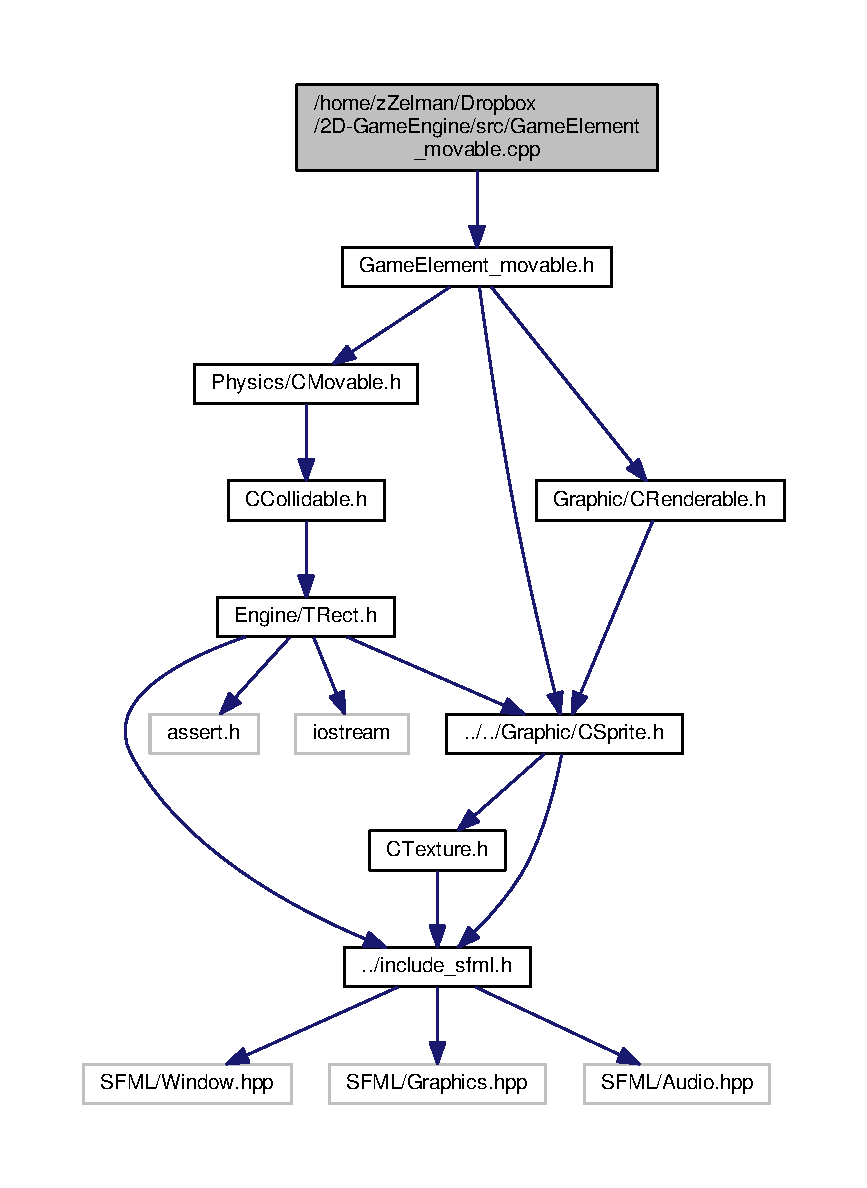
\includegraphics[width=350pt]{GameElement__movable_8cpp__incl}
\end{center}
\end{figure}

\hypertarget{GameElement__movable_8h}{\section{/home/z\-Zelman/\-Dropbox/2\-D-\/\-Game\-Engine/src/\-Game\-Element\-\_\-movable.h File Reference}
\label{GameElement__movable_8h}\index{/home/z\-Zelman/\-Dropbox/2\-D-\/\-Game\-Engine/src/\-Game\-Element\-\_\-movable.\-h@{/home/z\-Zelman/\-Dropbox/2\-D-\/\-Game\-Engine/src/\-Game\-Element\-\_\-movable.\-h}}
}
{\ttfamily \#include \char`\"{}Physics/\-C\-Movable.\-h\char`\"{}}\\*
{\ttfamily \#include \char`\"{}Graphic/\-C\-Sprite.\-h\char`\"{}}\\*
Include dependency graph for Game\-Element\-\_\-movable.\-h\-:\nopagebreak
\begin{figure}[H]
\begin{center}
\leavevmode
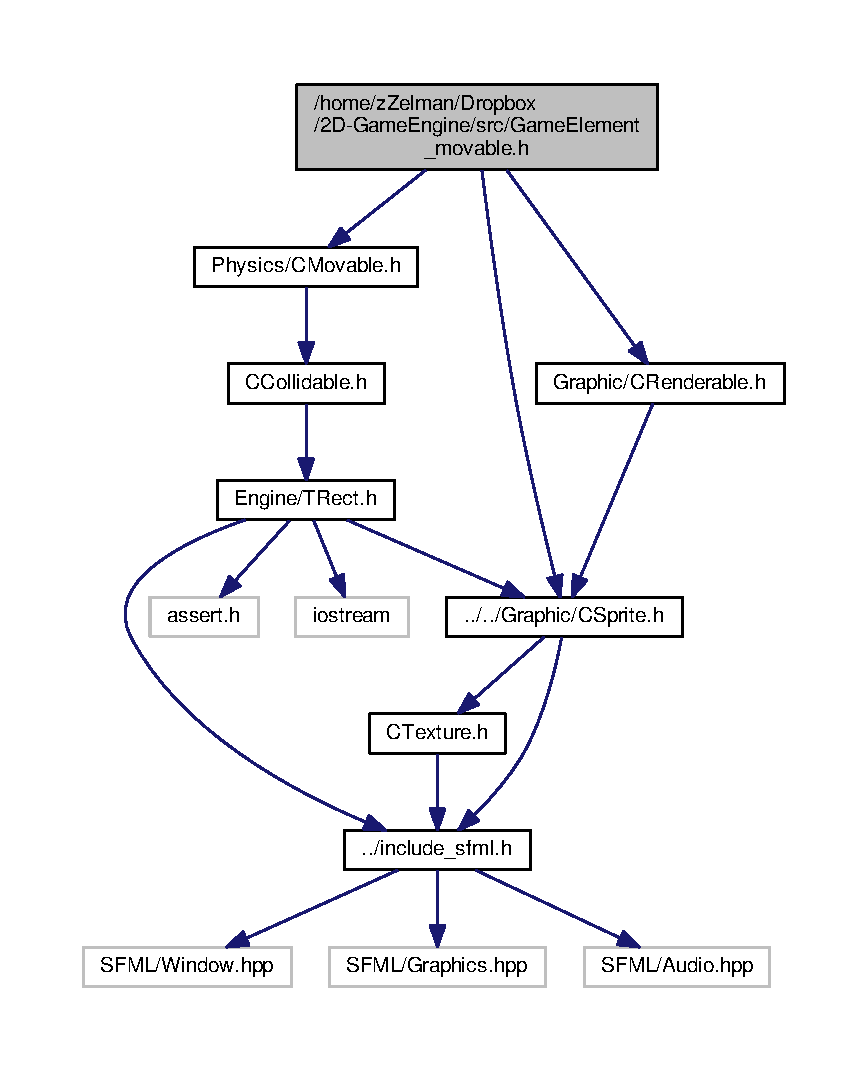
\includegraphics[width=350pt]{GameElement__movable_8h__incl}
\end{center}
\end{figure}
This graph shows which files directly or indirectly include this file\-:\nopagebreak
\begin{figure}[H]
\begin{center}
\leavevmode
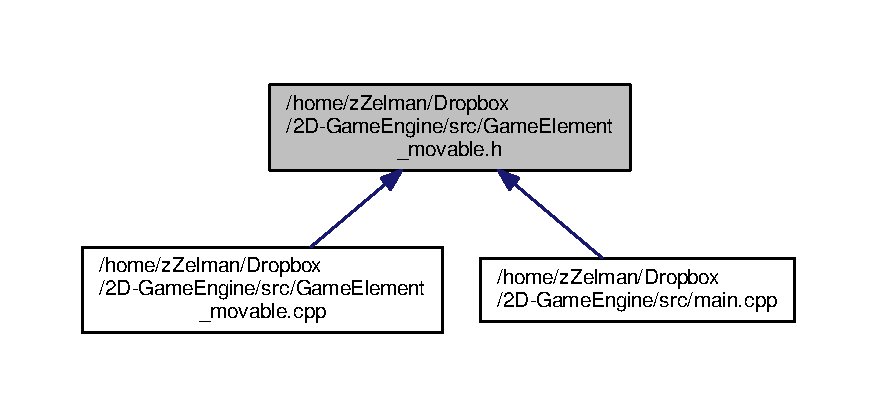
\includegraphics[width=350pt]{GameElement__movable_8h__dep__incl}
\end{center}
\end{figure}
\subsection*{Classes}
\begin{DoxyCompactItemize}
\item 
class \hyperlink{classGameElement__movable}{Game\-Element\-\_\-movable}
\end{DoxyCompactItemize}

\hypertarget{GameElement__static_8cpp}{\section{/home/z\-Zelman/\-Dropbox/2\-D-\/\-Game\-Engine/src/\-Game\-Element\-\_\-static.cpp File Reference}
\label{GameElement__static_8cpp}\index{/home/z\-Zelman/\-Dropbox/2\-D-\/\-Game\-Engine/src/\-Game\-Element\-\_\-static.\-cpp@{/home/z\-Zelman/\-Dropbox/2\-D-\/\-Game\-Engine/src/\-Game\-Element\-\_\-static.\-cpp}}
}
{\ttfamily \#include \char`\"{}Game\-Element\-\_\-static.\-h\char`\"{}}\\*
Include dependency graph for Game\-Element\-\_\-static.\-cpp\-:
\nopagebreak
\begin{figure}[H]
\begin{center}
\leavevmode
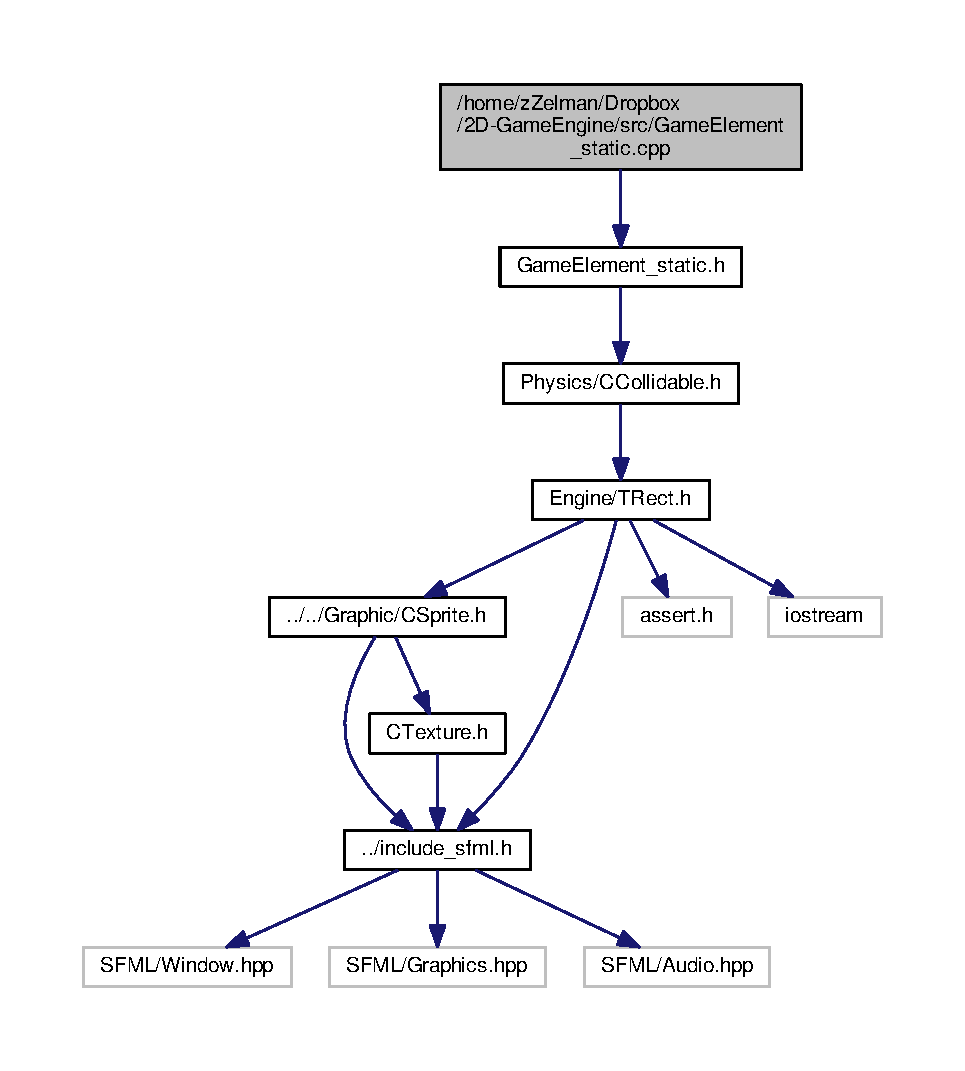
\includegraphics[width=350pt]{GameElement__static_8cpp__incl}
\end{center}
\end{figure}

\hypertarget{GameElement__static_8h}{\section{/home/z\-Zelman/\-Dropbox/2\-D-\/\-Game\-Engine/src/\-Game\-Element\-\_\-static.h File Reference}
\label{GameElement__static_8h}\index{/home/z\-Zelman/\-Dropbox/2\-D-\/\-Game\-Engine/src/\-Game\-Element\-\_\-static.\-h@{/home/z\-Zelman/\-Dropbox/2\-D-\/\-Game\-Engine/src/\-Game\-Element\-\_\-static.\-h}}
}
{\ttfamily \#include \char`\"{}Physics/\-C\-Collidable.\-h\char`\"{}}\\*
Include dependency graph for Game\-Element\-\_\-static.\-h\-:\nopagebreak
\begin{figure}[H]
\begin{center}
\leavevmode
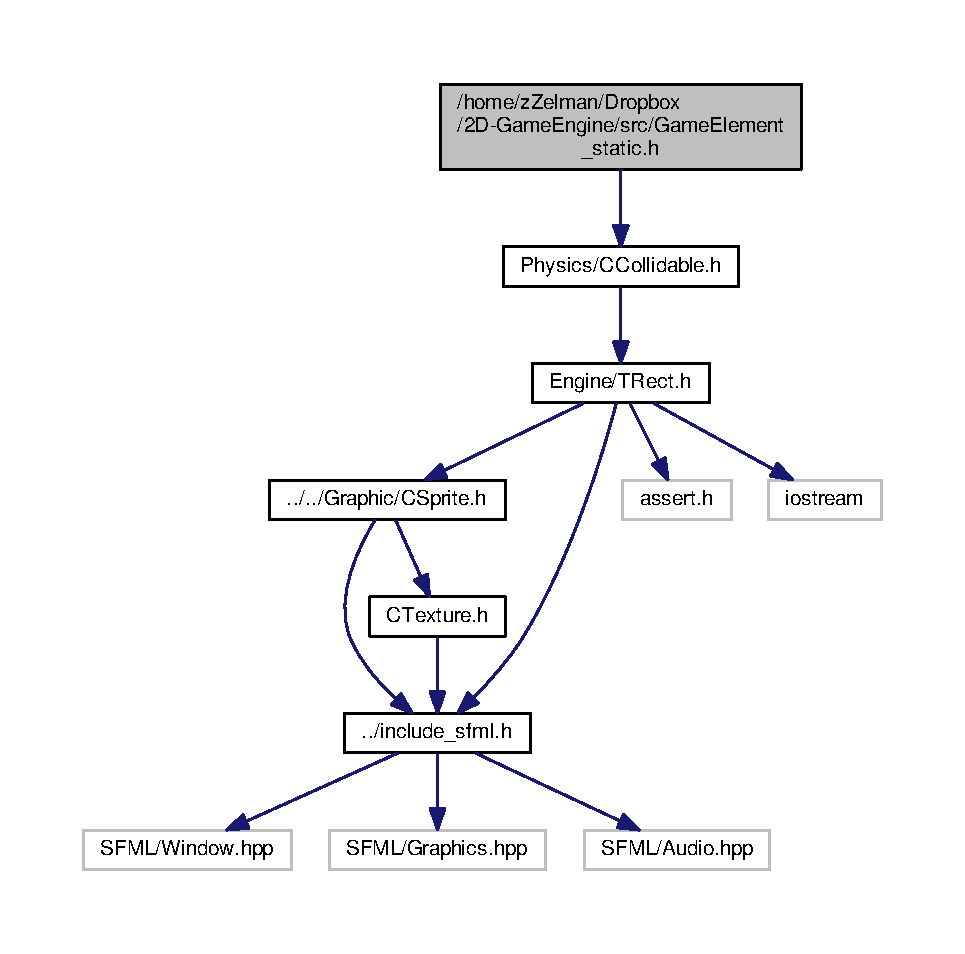
\includegraphics[width=350pt]{GameElement__static_8h__incl}
\end{center}
\end{figure}
This graph shows which files directly or indirectly include this file\-:\nopagebreak
\begin{figure}[H]
\begin{center}
\leavevmode
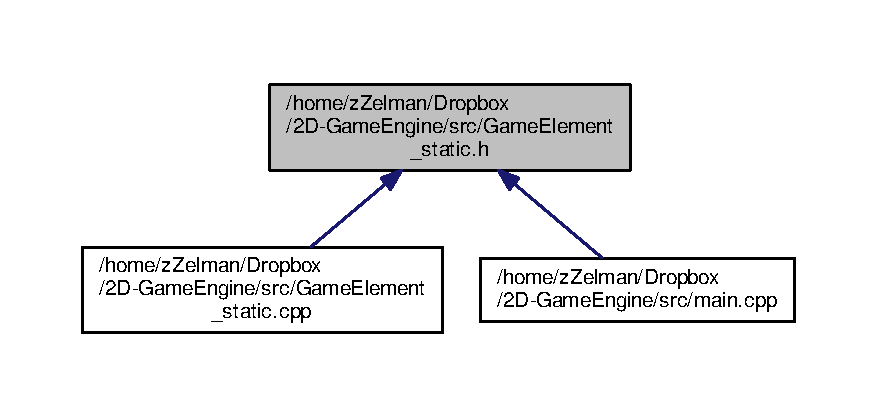
\includegraphics[width=350pt]{GameElement__static_8h__dep__incl}
\end{center}
\end{figure}
\subsection*{Classes}
\begin{DoxyCompactItemize}
\item 
class \hyperlink{classGameElement__static}{Game\-Element\-\_\-static}
\end{DoxyCompactItemize}

\hypertarget{CSprite_8cpp}{\section{/home/z\-Zelman/\-Dropbox/\-Marshmallow-\/\-Duels/src/\-Graphics/\-C\-Sprite.cpp File Reference}
\label{CSprite_8cpp}\index{/home/z\-Zelman/\-Dropbox/\-Marshmallow-\/\-Duels/src/\-Graphics/\-C\-Sprite.\-cpp@{/home/z\-Zelman/\-Dropbox/\-Marshmallow-\/\-Duels/src/\-Graphics/\-C\-Sprite.\-cpp}}
}
{\ttfamily \#include \char`\"{}../\-Headers/\-C\-Sprite.\-h\char`\"{}}\\*
{\ttfamily \#include \char`\"{}../\-Headers/include\-\_\-sfml.\-h\char`\"{}}\\*
{\ttfamily \#include $<$assert.\-h$>$}\\*
Include dependency graph for C\-Sprite.\-cpp\-:\nopagebreak
\begin{figure}[H]
\begin{center}
\leavevmode
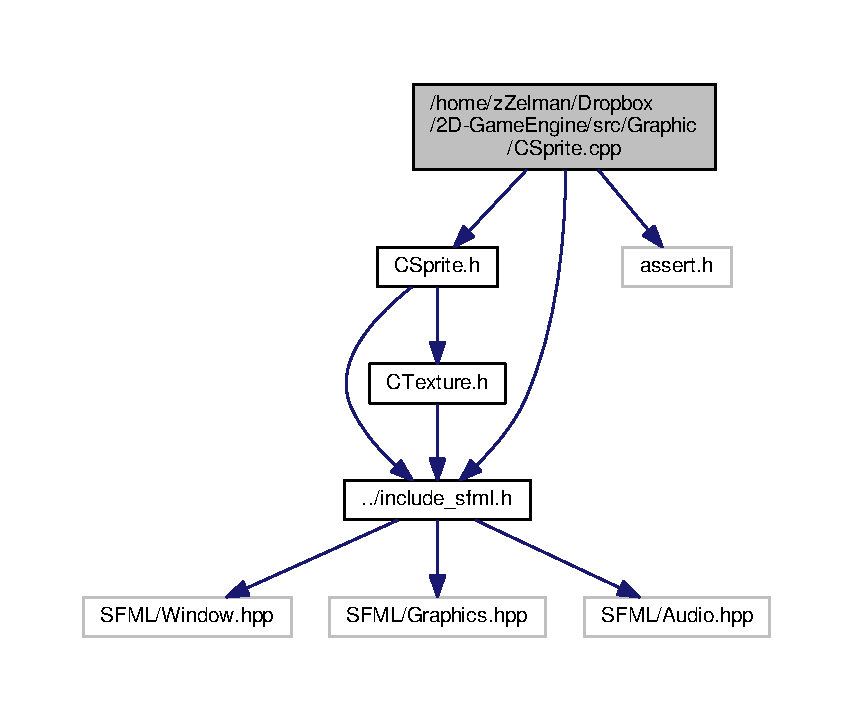
\includegraphics[width=350pt]{CSprite_8cpp__incl}
\end{center}
\end{figure}

\hypertarget{CSprite_8h}{\section{/home/z\-Zelman/\-Dropbox/2\-D-\/\-Game\-Engine/src/\-Graphic/\-C\-Sprite.h File Reference}
\label{CSprite_8h}\index{/home/z\-Zelman/\-Dropbox/2\-D-\/\-Game\-Engine/src/\-Graphic/\-C\-Sprite.\-h@{/home/z\-Zelman/\-Dropbox/2\-D-\/\-Game\-Engine/src/\-Graphic/\-C\-Sprite.\-h}}
}
{\ttfamily \#include \char`\"{}../include\-\_\-sfml.\-h\char`\"{}}\\*
{\ttfamily \#include \char`\"{}C\-Texture.\-h\char`\"{}}\\*
Include dependency graph for C\-Sprite.\-h\-:
\nopagebreak
\begin{figure}[H]
\begin{center}
\leavevmode
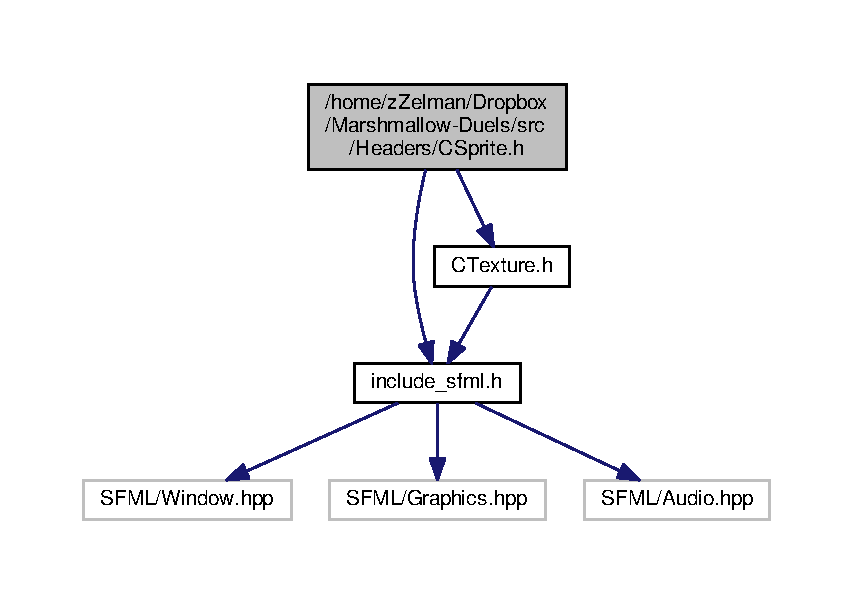
\includegraphics[width=350pt]{CSprite_8h__incl}
\end{center}
\end{figure}
This graph shows which files directly or indirectly include this file\-:
\nopagebreak
\begin{figure}[H]
\begin{center}
\leavevmode
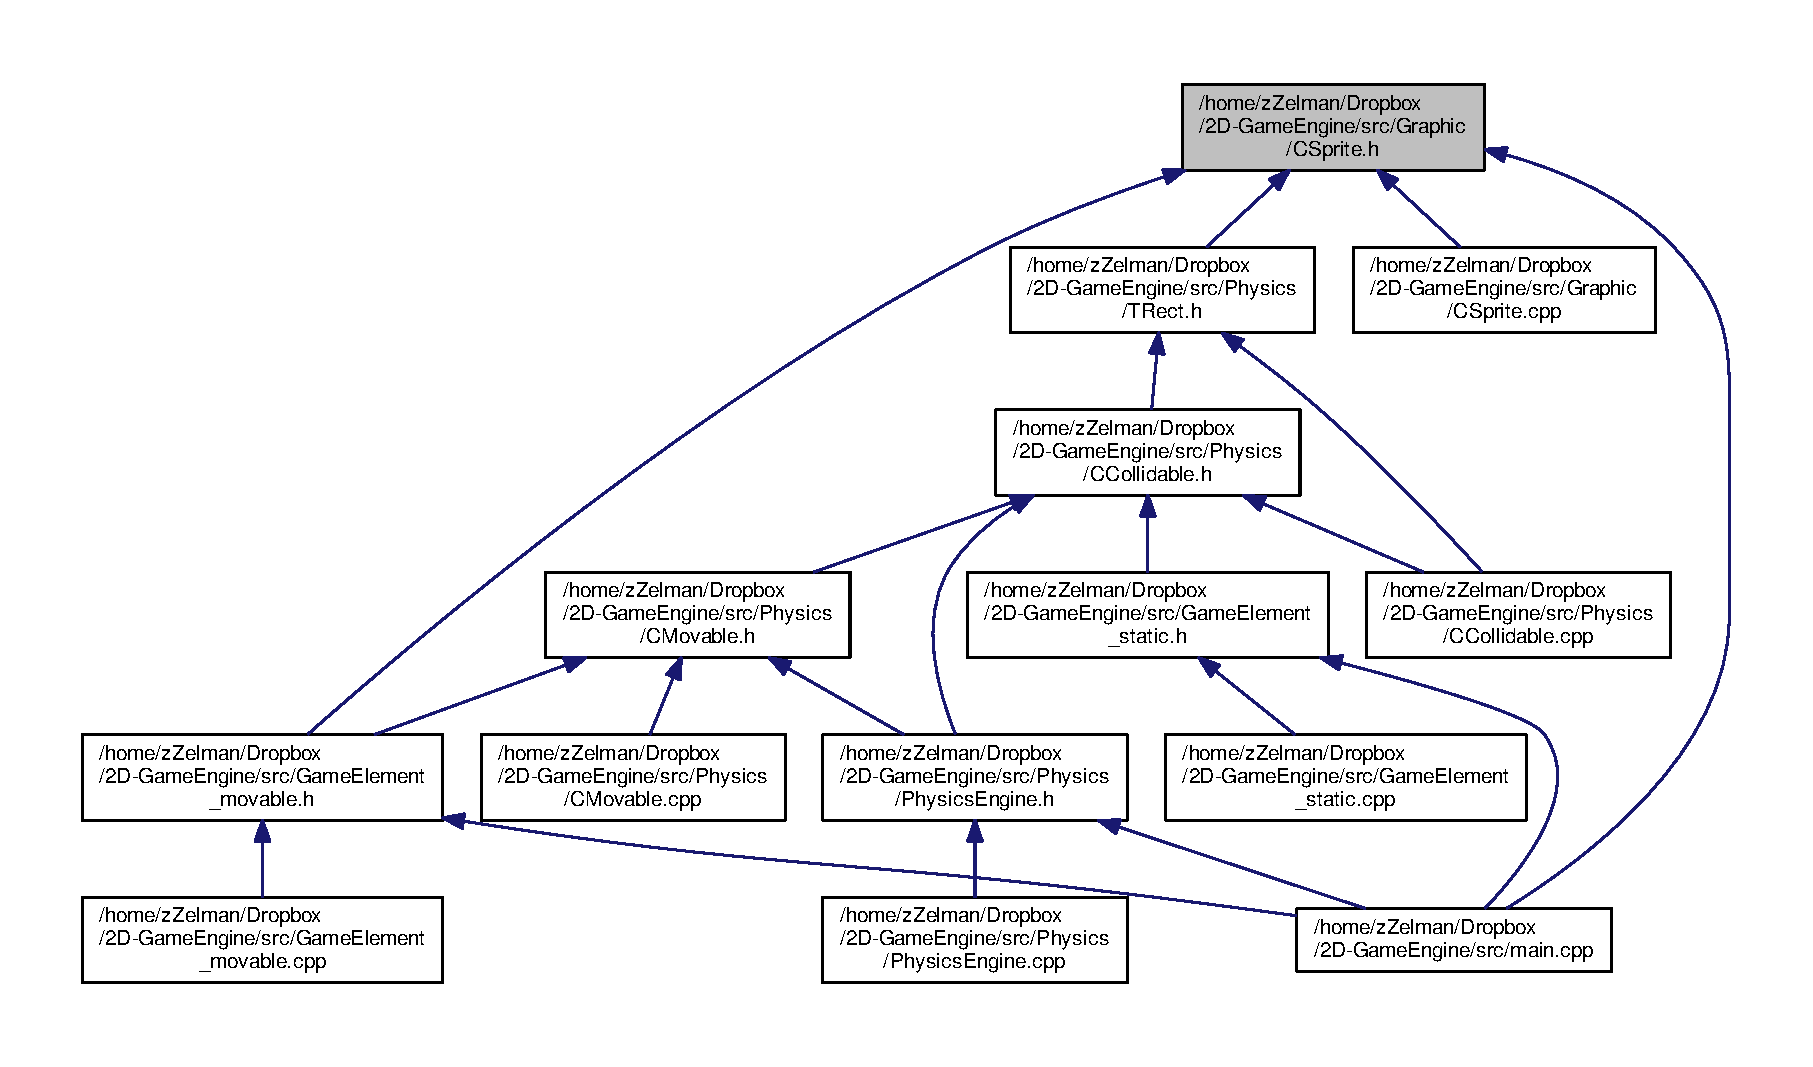
\includegraphics[width=350pt]{CSprite_8h__dep__incl}
\end{center}
\end{figure}
\subsection*{Classes}
\begin{DoxyCompactItemize}
\item 
class \hyperlink{classCSprite}{C\-Sprite}
\begin{DoxyCompactList}\small\item\em Wrapper class for S\-F\-M\-L 2.\-1 Sprite. \end{DoxyCompactList}\end{DoxyCompactItemize}

\hypertarget{CTexture_8cpp}{\section{/home/z\-Zelman/\-Dropbox/2\-D-\/\-Game\-Engine/src/\-Graphic/\-C\-Texture.cpp File Reference}
\label{CTexture_8cpp}\index{/home/z\-Zelman/\-Dropbox/2\-D-\/\-Game\-Engine/src/\-Graphic/\-C\-Texture.\-cpp@{/home/z\-Zelman/\-Dropbox/2\-D-\/\-Game\-Engine/src/\-Graphic/\-C\-Texture.\-cpp}}
}
{\ttfamily \#include \char`\"{}C\-Texture.\-h\char`\"{}}\\*
{\ttfamily \#include \char`\"{}../include\-\_\-sfml.\-h\char`\"{}}\\*
{\ttfamily \#include $<$assert.\-h$>$}\\*
Include dependency graph for C\-Texture.\-cpp\-:
\nopagebreak
\begin{figure}[H]
\begin{center}
\leavevmode
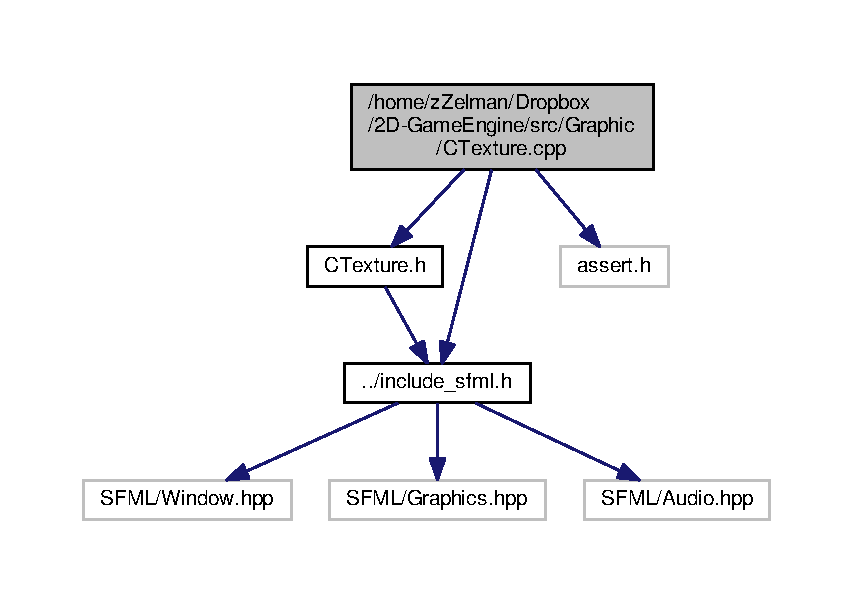
\includegraphics[width=350pt]{CTexture_8cpp__incl}
\end{center}
\end{figure}

\hypertarget{CTexture_8h}{\section{/home/z\-Zelman/\-Dropbox/2\-D-\/\-Game\-Engine/src/\-Graphic/\-C\-Texture.h File Reference}
\label{CTexture_8h}\index{/home/z\-Zelman/\-Dropbox/2\-D-\/\-Game\-Engine/src/\-Graphic/\-C\-Texture.\-h@{/home/z\-Zelman/\-Dropbox/2\-D-\/\-Game\-Engine/src/\-Graphic/\-C\-Texture.\-h}}
}
{\ttfamily \#include \char`\"{}../include\-\_\-sfml.\-h\char`\"{}}\\*
Include dependency graph for C\-Texture.\-h\-:\nopagebreak
\begin{figure}[H]
\begin{center}
\leavevmode
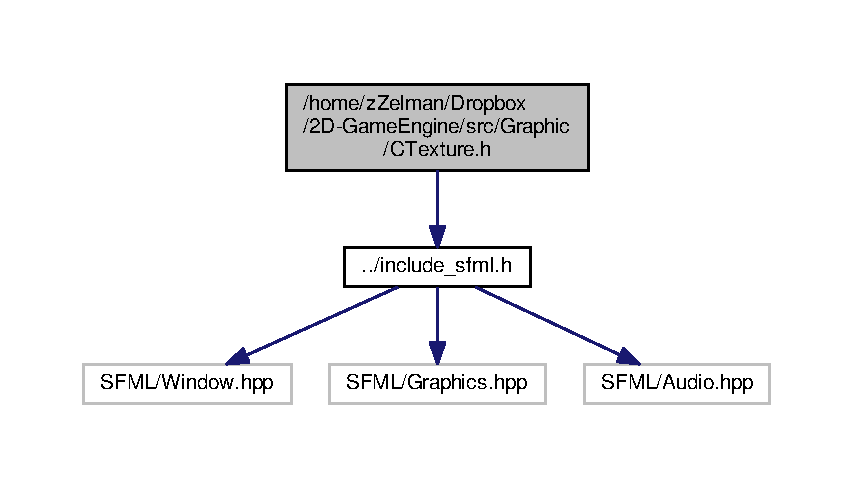
\includegraphics[width=350pt]{CTexture_8h__incl}
\end{center}
\end{figure}
This graph shows which files directly or indirectly include this file\-:\nopagebreak
\begin{figure}[H]
\begin{center}
\leavevmode
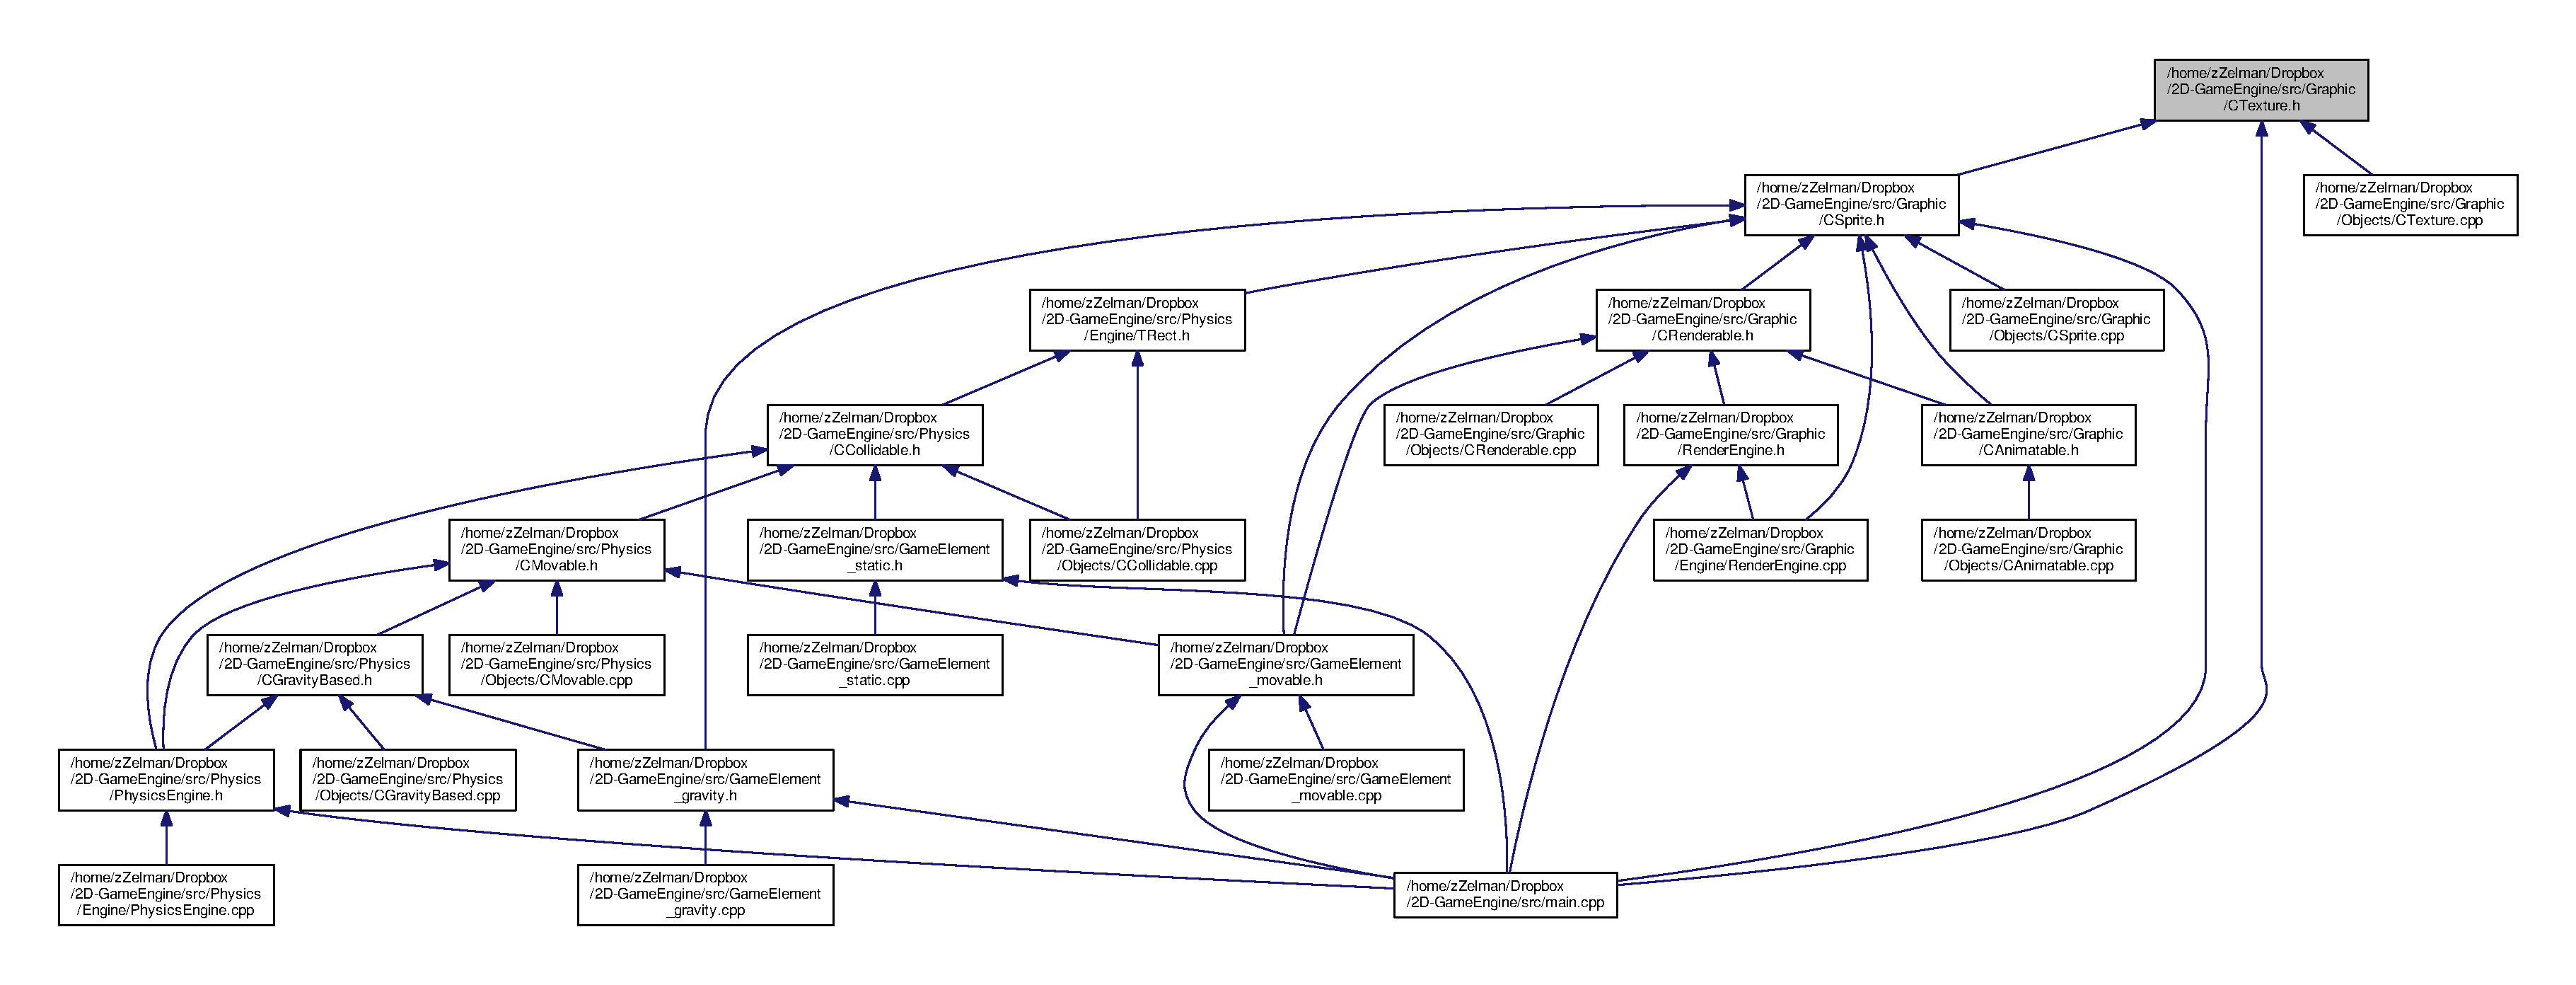
\includegraphics[width=350pt]{CTexture_8h__dep__incl}
\end{center}
\end{figure}
\subsection*{Classes}
\begin{DoxyCompactItemize}
\item 
class \hyperlink{classCTexture}{C\-Texture}
\begin{DoxyCompactList}\small\item\em Wrapper class for S\-F\-M\-L 2.\-1 Texture. \end{DoxyCompactList}\end{DoxyCompactItemize}

\hypertarget{include__sfml_8h}{\section{/home/z\-Zelman/\-Dropbox/2\-D-\/\-Game\-Engine/src/include\-\_\-sfml.h File Reference}
\label{include__sfml_8h}\index{/home/z\-Zelman/\-Dropbox/2\-D-\/\-Game\-Engine/src/include\-\_\-sfml.\-h@{/home/z\-Zelman/\-Dropbox/2\-D-\/\-Game\-Engine/src/include\-\_\-sfml.\-h}}
}
{\ttfamily \#include $<$S\-F\-M\-L/\-Window.\-hpp$>$}\\*
{\ttfamily \#include $<$S\-F\-M\-L/\-Graphics.\-hpp$>$}\\*
{\ttfamily \#include $<$S\-F\-M\-L/\-Audio.\-hpp$>$}\\*
Include dependency graph for include\-\_\-sfml.\-h\-:
\nopagebreak
\begin{figure}[H]
\begin{center}
\leavevmode
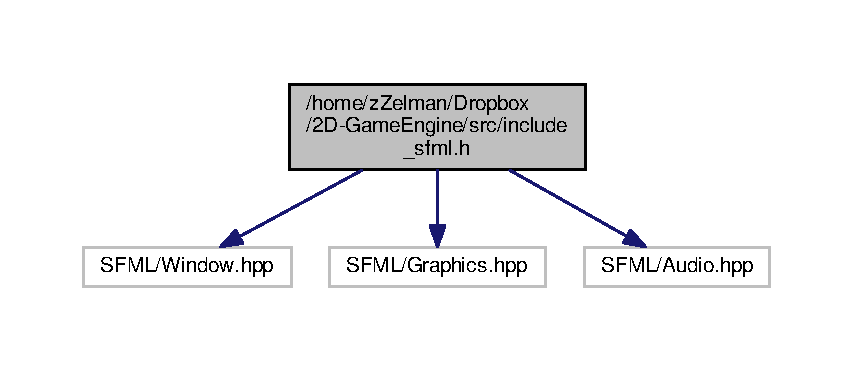
\includegraphics[width=350pt]{include__sfml_8h__incl}
\end{center}
\end{figure}
This graph shows which files directly or indirectly include this file\-:
\nopagebreak
\begin{figure}[H]
\begin{center}
\leavevmode
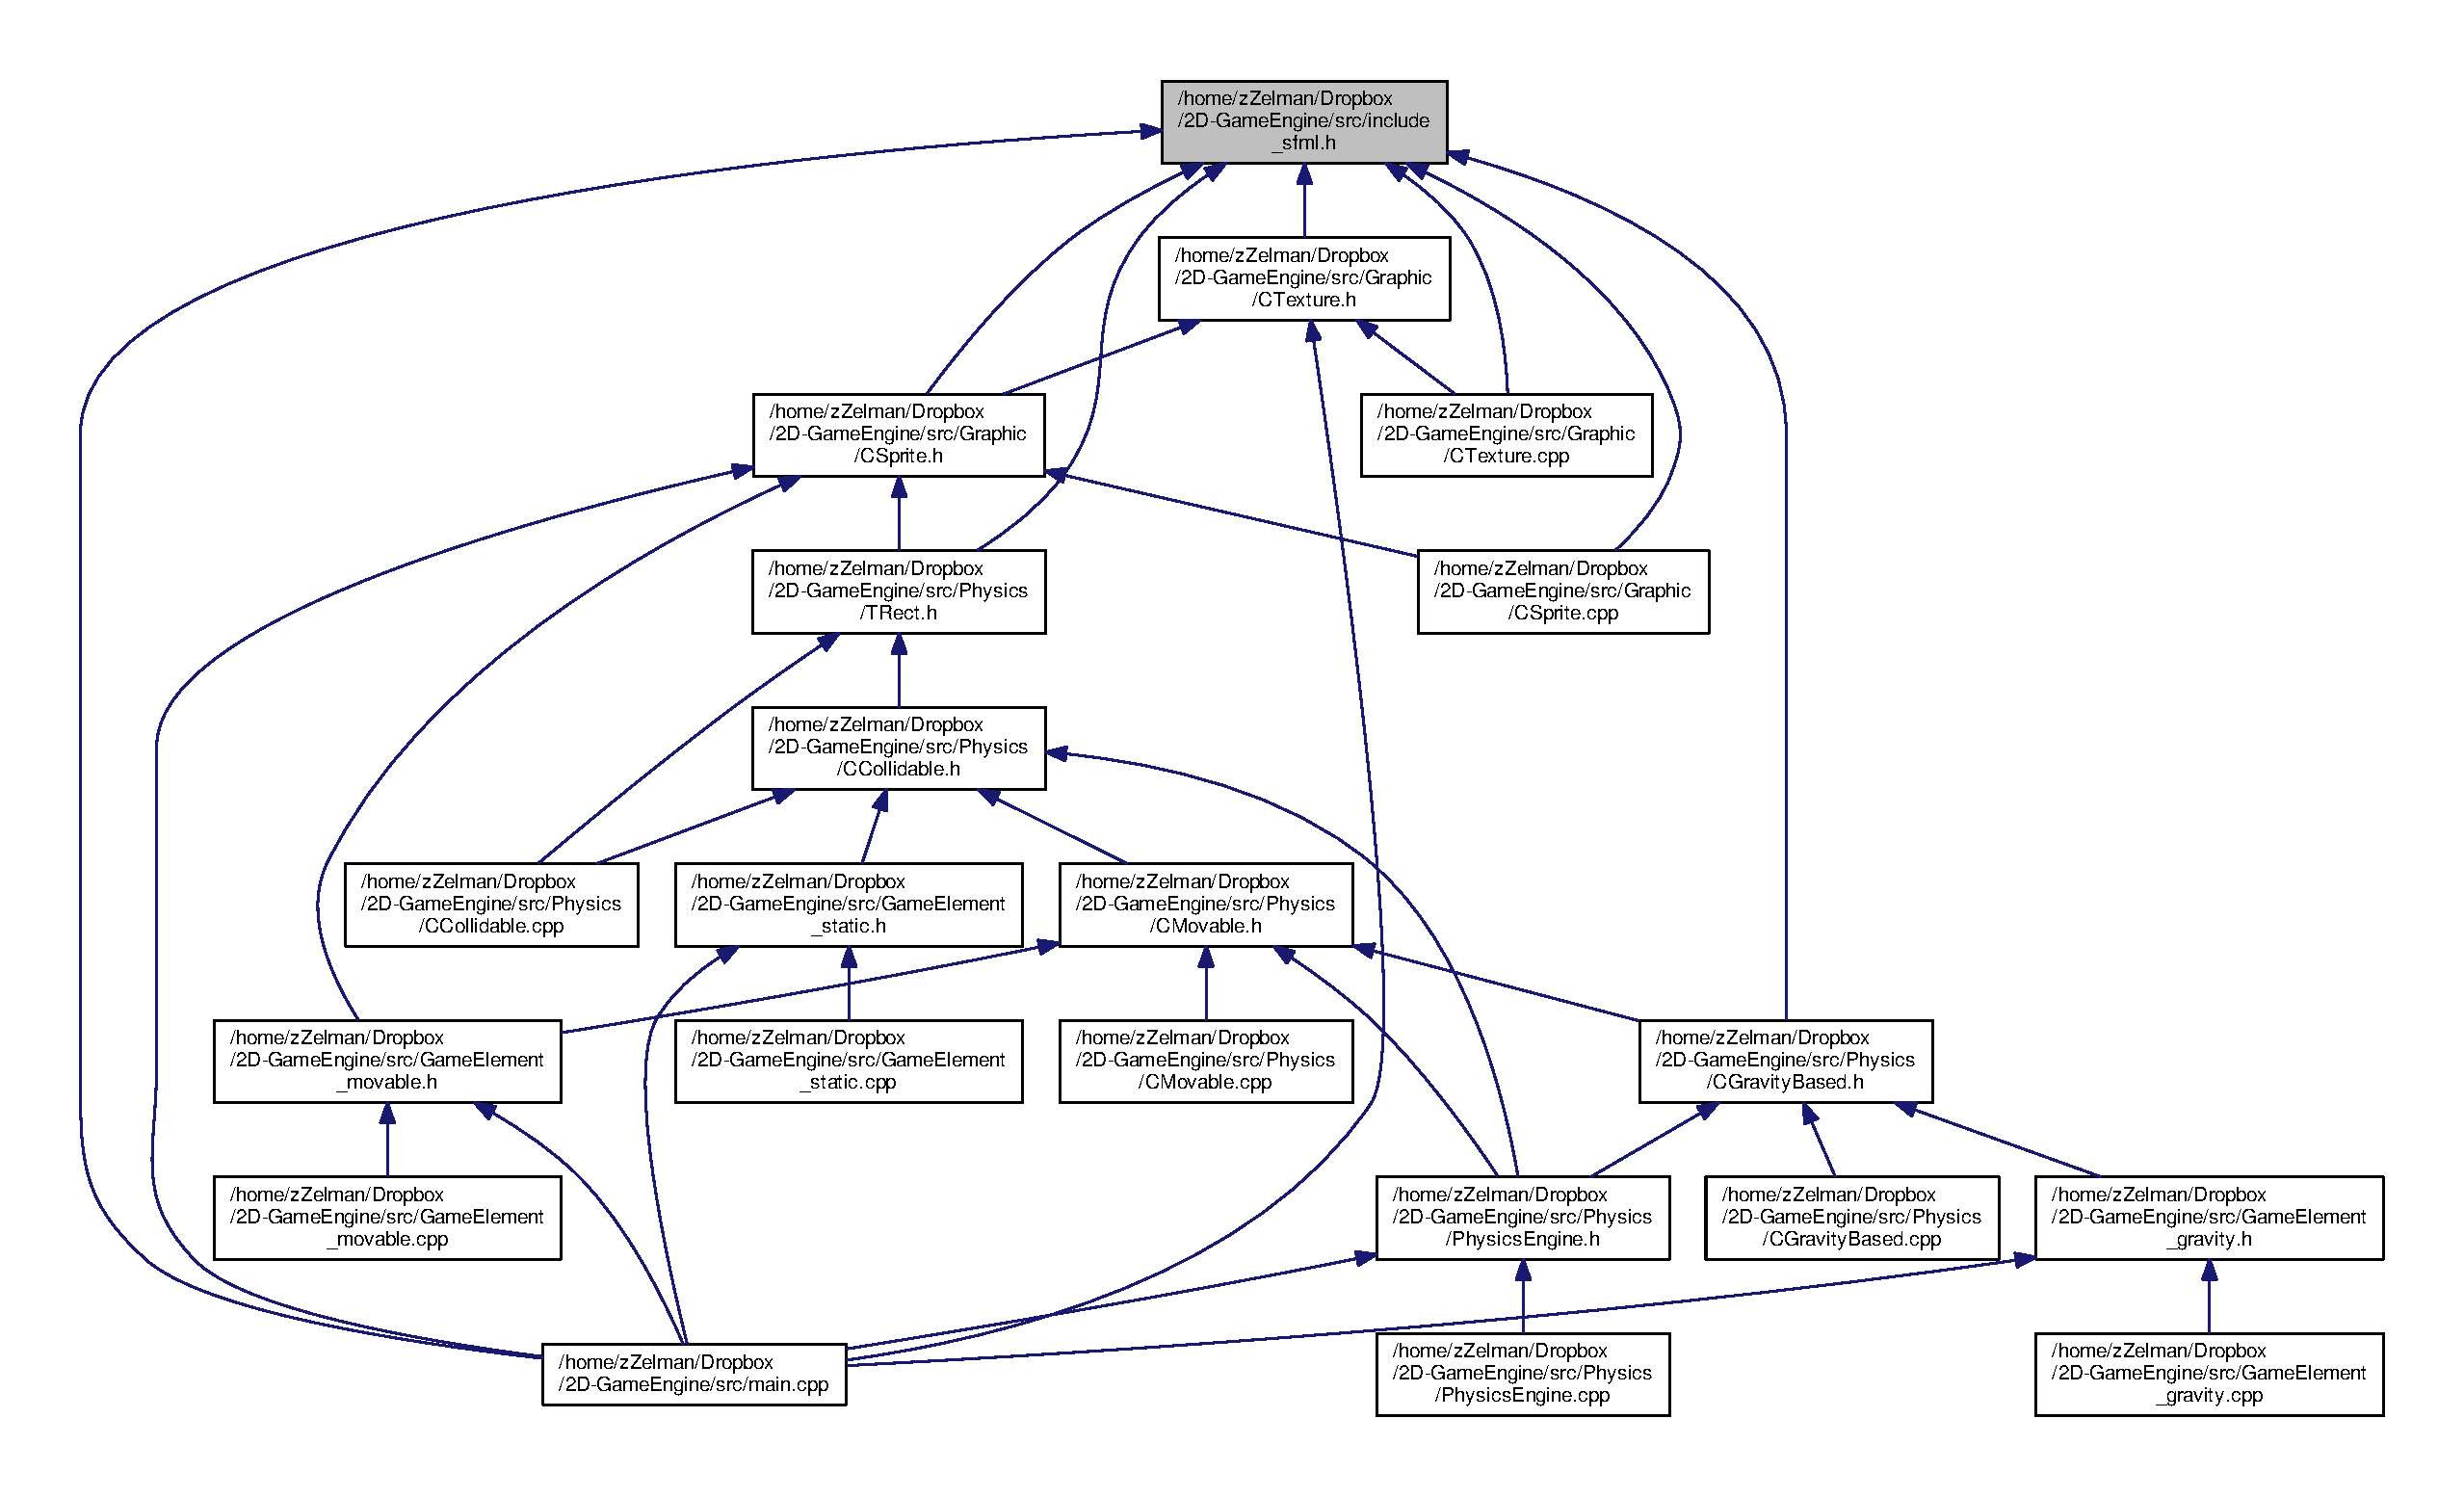
\includegraphics[width=230pt]{include__sfml_8h__dep__incl}
\end{center}
\end{figure}

\hypertarget{main_8cpp}{\section{/home/z\-Zelman/\-Dropbox/2\-D-\/\-Game\-Engine/src/main.cpp File Reference}
\label{main_8cpp}\index{/home/z\-Zelman/\-Dropbox/2\-D-\/\-Game\-Engine/src/main.\-cpp@{/home/z\-Zelman/\-Dropbox/2\-D-\/\-Game\-Engine/src/main.\-cpp}}
}
{\ttfamily \#include \char`\"{}include\-\_\-sfml.\-h\char`\"{}}\\*
{\ttfamily \#include \char`\"{}Graphic/\-C\-Texture.\-h\char`\"{}}\\*
{\ttfamily \#include \char`\"{}Graphic/\-C\-Sprite.\-h\char`\"{}}\\*
{\ttfamily \#include \char`\"{}Game\-Element\-\_\-movable.\-h\char`\"{}}\\*
{\ttfamily \#include \char`\"{}Game\-Element\-\_\-static.\-h\char`\"{}}\\*
{\ttfamily \#include \char`\"{}Physics/\-Physics\-Engine.\-h\char`\"{}}\\*
Include dependency graph for main.\-cpp\-:
\nopagebreak
\begin{figure}[H]
\begin{center}
\leavevmode
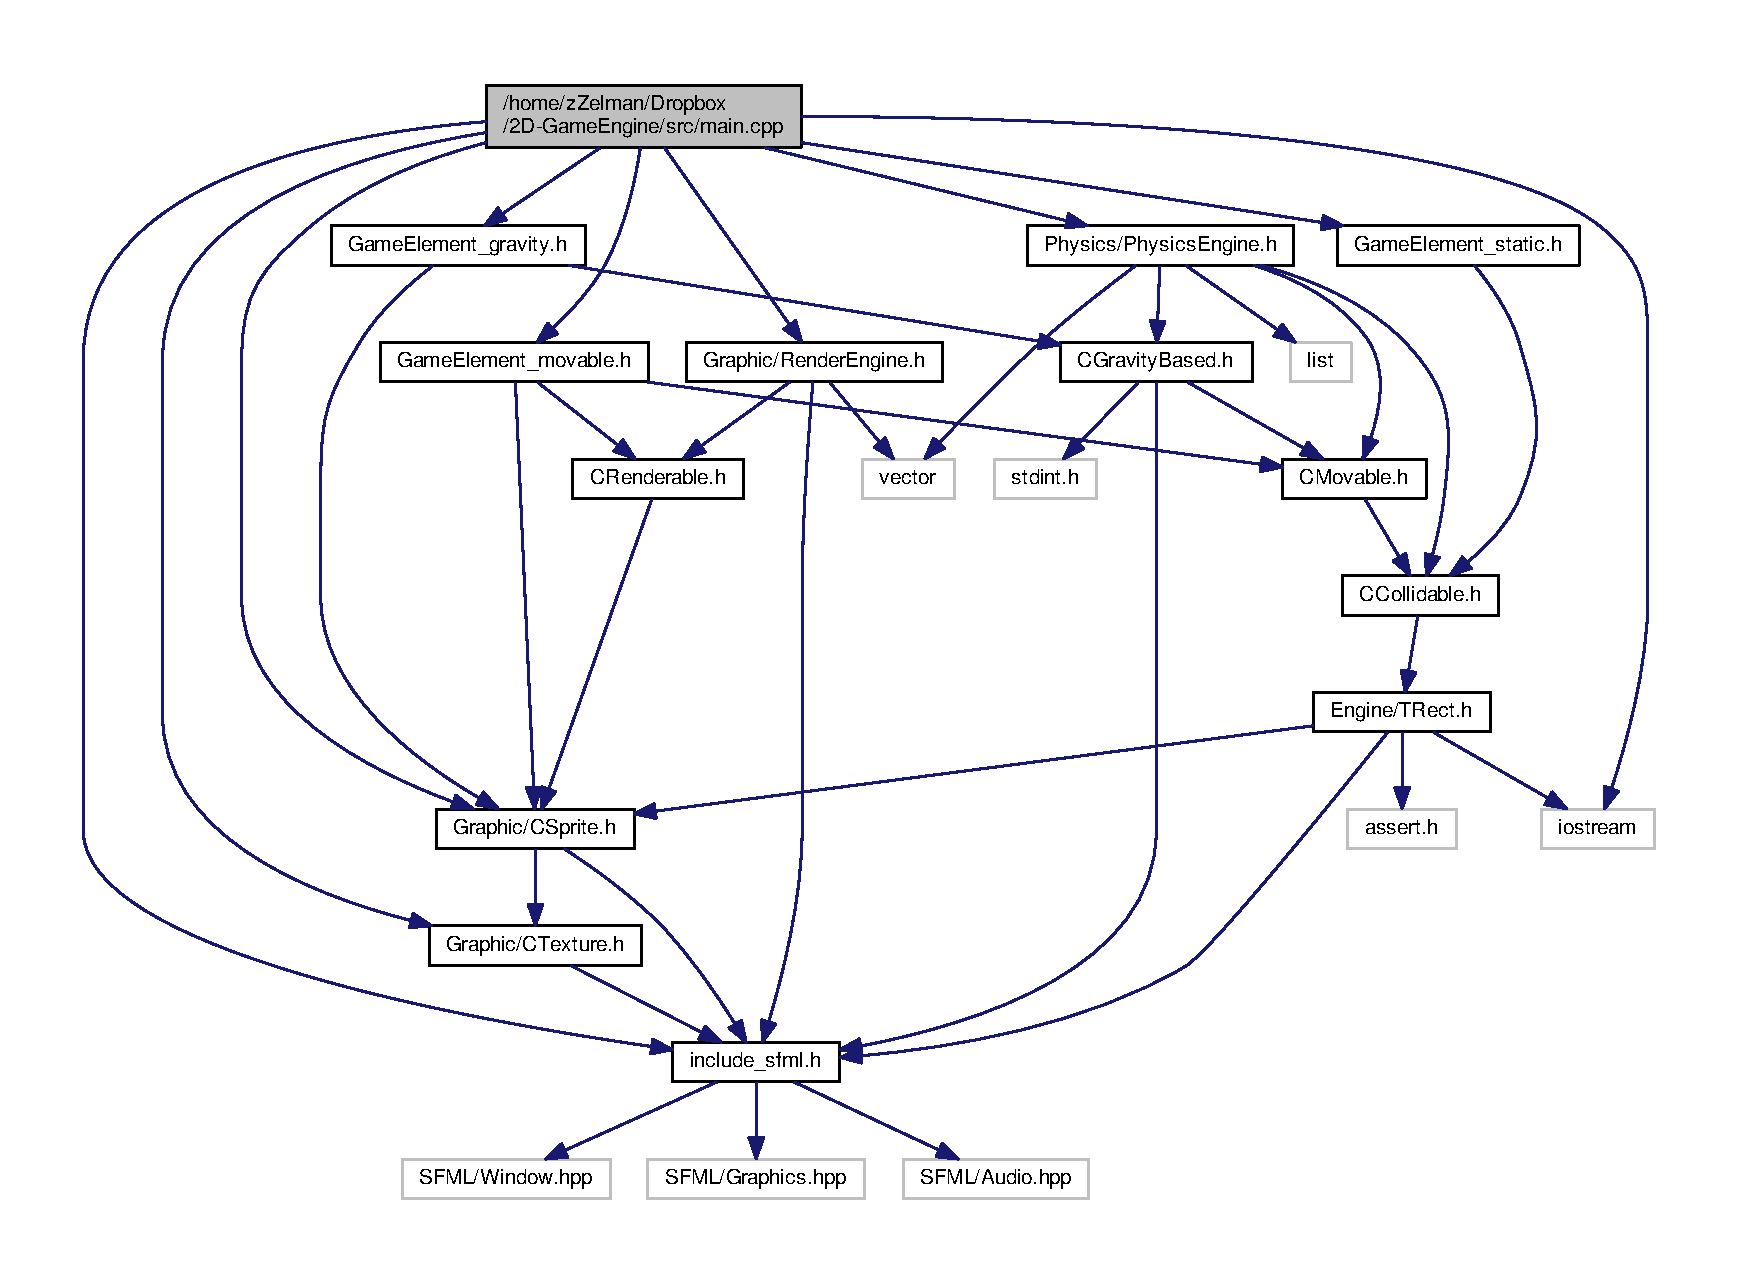
\includegraphics[width=350pt]{main_8cpp__incl}
\end{center}
\end{figure}
\subsection*{Functions}
\begin{DoxyCompactItemize}
\item 
void \hyperlink{main_8cpp_a0a462ec35bf9c8a31ea7b4c653ab3f4c}{window\-\_\-events} (bool \&done)
\begin{DoxyCompactList}\small\item\em Simplistic window event handling. \end{DoxyCompactList}\item 
void \hyperlink{main_8cpp_a6bbf2b1b4a5441f0205c3258bd661077}{update\-\_\-elements} ()
\begin{DoxyCompactList}\small\item\em Simplistic updating. \end{DoxyCompactList}\item 
void \hyperlink{main_8cpp_a20e3a3051df36234b0ce05ffac0741ee}{render\-\_\-elements} ()
\begin{DoxyCompactList}\small\item\em Simplistic rendering. \end{DoxyCompactList}\item 
void \hyperlink{main_8cpp_a190163a6c0c635f4695f2fdd61d2cb8c}{init\-\_\-elements} ()
\begin{DoxyCompactList}\small\item\em Init unit testing objects. \end{DoxyCompactList}\item 
void \hyperlink{main_8cpp_a4e306517e52618c9e9ba61f2beae2f94}{delete\-\_\-elements} ()
\begin{DoxyCompactList}\small\item\em Delete unit testing objects. \end{DoxyCompactList}\item 
int \hyperlink{main_8cpp_a0ddf1224851353fc92bfbff6f499fa97}{main} (int argc, char $\ast$argv\mbox{[}$\,$\mbox{]})
\begin{DoxyCompactList}\small\item\em Start of program. \end{DoxyCompactList}\end{DoxyCompactItemize}
\subsection*{Variables}
\begin{DoxyCompactItemize}
\item 
sf\-::\-Render\-Window $\ast$ \hyperlink{main_8cpp_a09bf53be0697112e73cc7ceaca479ef6}{g\-\_\-window}
\item 
\hyperlink{classCTexture}{C\-Texture} $\ast$ \hyperlink{main_8cpp_a7e2879f22f371962a365e7c8d9f0699f}{g\-\_\-texture}
\item 
\hyperlink{classCSprite}{C\-Sprite} $\ast$ \hyperlink{main_8cpp_a68ec2c6cb385b95c73463cbeeb11759d}{g\-\_\-sprite\-\_\-movable}
\item 
\hyperlink{classGameElement__movable}{Game\-Element\-\_\-movable} $\ast$ \hyperlink{main_8cpp_ab43805fb979ee1bdb9fa4ef8500736f5}{g\-\_\-element\-\_\-movable}
\item 
\hyperlink{classCSprite}{C\-Sprite} $\ast$ \hyperlink{main_8cpp_acb23cd68aed5278e47711f5b62734397}{g\-\_\-sprite\-\_\-static}
\item 
\hyperlink{classGameElement__static}{Game\-Element\-\_\-static} $\ast$ \hyperlink{main_8cpp_aff6119240a4bf77d3a20abd24127b596}{g\-\_\-element\-\_\-static}
\item 
\hyperlink{classengine_1_1PhysicsEngine}{engine\-::\-Physics\-Engine} $\ast$ \hyperlink{main_8cpp_aee1bcd5912424a8845145c705c1e3e39}{g\-\_\-physics\-Engine}
\end{DoxyCompactItemize}


\subsection{Function Documentation}
\hypertarget{main_8cpp_a4e306517e52618c9e9ba61f2beae2f94}{\index{main.\-cpp@{main.\-cpp}!delete\-\_\-elements@{delete\-\_\-elements}}
\index{delete\-\_\-elements@{delete\-\_\-elements}!main.cpp@{main.\-cpp}}
\subsubsection[{delete\-\_\-elements}]{\setlength{\rightskip}{0pt plus 5cm}void delete\-\_\-elements (
\begin{DoxyParamCaption}
{}
\end{DoxyParamCaption}
)}}\label{main_8cpp_a4e306517e52618c9e9ba61f2beae2f94}


Delete unit testing objects. 



Definition at line 135 of file main.\-cpp.

\hypertarget{main_8cpp_a190163a6c0c635f4695f2fdd61d2cb8c}{\index{main.\-cpp@{main.\-cpp}!init\-\_\-elements@{init\-\_\-elements}}
\index{init\-\_\-elements@{init\-\_\-elements}!main.cpp@{main.\-cpp}}
\subsubsection[{init\-\_\-elements}]{\setlength{\rightskip}{0pt plus 5cm}void init\-\_\-elements (
\begin{DoxyParamCaption}
{}
\end{DoxyParamCaption}
)}}\label{main_8cpp_a190163a6c0c635f4695f2fdd61d2cb8c}


Init unit testing objects. 



Definition at line 110 of file main.\-cpp.

\hypertarget{main_8cpp_a0ddf1224851353fc92bfbff6f499fa97}{\index{main.\-cpp@{main.\-cpp}!main@{main}}
\index{main@{main}!main.cpp@{main.\-cpp}}
\subsubsection[{main}]{\setlength{\rightskip}{0pt plus 5cm}int main (
\begin{DoxyParamCaption}
\item[{int}]{argc, }
\item[{char $\ast$}]{argv\mbox{[}$\,$\mbox{]}}
\end{DoxyParamCaption}
)}}\label{main_8cpp_a0ddf1224851353fc92bfbff6f499fa97}


Start of program. 



Definition at line 154 of file main.\-cpp.

\hypertarget{main_8cpp_a20e3a3051df36234b0ce05ffac0741ee}{\index{main.\-cpp@{main.\-cpp}!render\-\_\-elements@{render\-\_\-elements}}
\index{render\-\_\-elements@{render\-\_\-elements}!main.cpp@{main.\-cpp}}
\subsubsection[{render\-\_\-elements}]{\setlength{\rightskip}{0pt plus 5cm}void render\-\_\-elements (
\begin{DoxyParamCaption}
{}
\end{DoxyParamCaption}
)}}\label{main_8cpp_a20e3a3051df36234b0ce05ffac0741ee}


Simplistic rendering. 



Definition at line 97 of file main.\-cpp.

\hypertarget{main_8cpp_a6bbf2b1b4a5441f0205c3258bd661077}{\index{main.\-cpp@{main.\-cpp}!update\-\_\-elements@{update\-\_\-elements}}
\index{update\-\_\-elements@{update\-\_\-elements}!main.cpp@{main.\-cpp}}
\subsubsection[{update\-\_\-elements}]{\setlength{\rightskip}{0pt plus 5cm}void update\-\_\-elements (
\begin{DoxyParamCaption}
{}
\end{DoxyParamCaption}
)}}\label{main_8cpp_a6bbf2b1b4a5441f0205c3258bd661077}


Simplistic updating. 



Definition at line 88 of file main.\-cpp.

\hypertarget{main_8cpp_a0a462ec35bf9c8a31ea7b4c653ab3f4c}{\index{main.\-cpp@{main.\-cpp}!window\-\_\-events@{window\-\_\-events}}
\index{window\-\_\-events@{window\-\_\-events}!main.cpp@{main.\-cpp}}
\subsubsection[{window\-\_\-events}]{\setlength{\rightskip}{0pt plus 5cm}void window\-\_\-events (
\begin{DoxyParamCaption}
\item[{bool \&}]{done}
\end{DoxyParamCaption}
)}}\label{main_8cpp_a0a462ec35bf9c8a31ea7b4c653ab3f4c}


Simplistic window event handling. 



Definition at line 22 of file main.\-cpp.



\subsection{Variable Documentation}
\hypertarget{main_8cpp_ab43805fb979ee1bdb9fa4ef8500736f5}{\index{main.\-cpp@{main.\-cpp}!g\-\_\-element\-\_\-movable@{g\-\_\-element\-\_\-movable}}
\index{g\-\_\-element\-\_\-movable@{g\-\_\-element\-\_\-movable}!main.cpp@{main.\-cpp}}
\subsubsection[{g\-\_\-element\-\_\-movable}]{\setlength{\rightskip}{0pt plus 5cm}{\bf Game\-Element\-\_\-movable}$\ast$ g\-\_\-element\-\_\-movable}}\label{main_8cpp_ab43805fb979ee1bdb9fa4ef8500736f5}


Definition at line 12 of file main.\-cpp.

\hypertarget{main_8cpp_aff6119240a4bf77d3a20abd24127b596}{\index{main.\-cpp@{main.\-cpp}!g\-\_\-element\-\_\-static@{g\-\_\-element\-\_\-static}}
\index{g\-\_\-element\-\_\-static@{g\-\_\-element\-\_\-static}!main.cpp@{main.\-cpp}}
\subsubsection[{g\-\_\-element\-\_\-static}]{\setlength{\rightskip}{0pt plus 5cm}{\bf Game\-Element\-\_\-static}$\ast$ g\-\_\-element\-\_\-static}}\label{main_8cpp_aff6119240a4bf77d3a20abd24127b596}


Definition at line 15 of file main.\-cpp.

\hypertarget{main_8cpp_aee1bcd5912424a8845145c705c1e3e39}{\index{main.\-cpp@{main.\-cpp}!g\-\_\-physics\-Engine@{g\-\_\-physics\-Engine}}
\index{g\-\_\-physics\-Engine@{g\-\_\-physics\-Engine}!main.cpp@{main.\-cpp}}
\subsubsection[{g\-\_\-physics\-Engine}]{\setlength{\rightskip}{0pt plus 5cm}{\bf engine\-::\-Physics\-Engine}$\ast$ g\-\_\-physics\-Engine}}\label{main_8cpp_aee1bcd5912424a8845145c705c1e3e39}


Definition at line 17 of file main.\-cpp.

\hypertarget{main_8cpp_a68ec2c6cb385b95c73463cbeeb11759d}{\index{main.\-cpp@{main.\-cpp}!g\-\_\-sprite\-\_\-movable@{g\-\_\-sprite\-\_\-movable}}
\index{g\-\_\-sprite\-\_\-movable@{g\-\_\-sprite\-\_\-movable}!main.cpp@{main.\-cpp}}
\subsubsection[{g\-\_\-sprite\-\_\-movable}]{\setlength{\rightskip}{0pt plus 5cm}{\bf C\-Sprite}$\ast$ g\-\_\-sprite\-\_\-movable}}\label{main_8cpp_a68ec2c6cb385b95c73463cbeeb11759d}


Definition at line 11 of file main.\-cpp.

\hypertarget{main_8cpp_acb23cd68aed5278e47711f5b62734397}{\index{main.\-cpp@{main.\-cpp}!g\-\_\-sprite\-\_\-static@{g\-\_\-sprite\-\_\-static}}
\index{g\-\_\-sprite\-\_\-static@{g\-\_\-sprite\-\_\-static}!main.cpp@{main.\-cpp}}
\subsubsection[{g\-\_\-sprite\-\_\-static}]{\setlength{\rightskip}{0pt plus 5cm}{\bf C\-Sprite}$\ast$ g\-\_\-sprite\-\_\-static}}\label{main_8cpp_acb23cd68aed5278e47711f5b62734397}


Definition at line 14 of file main.\-cpp.

\hypertarget{main_8cpp_a7e2879f22f371962a365e7c8d9f0699f}{\index{main.\-cpp@{main.\-cpp}!g\-\_\-texture@{g\-\_\-texture}}
\index{g\-\_\-texture@{g\-\_\-texture}!main.cpp@{main.\-cpp}}
\subsubsection[{g\-\_\-texture}]{\setlength{\rightskip}{0pt plus 5cm}{\bf C\-Texture}$\ast$ g\-\_\-texture}}\label{main_8cpp_a7e2879f22f371962a365e7c8d9f0699f}


Definition at line 9 of file main.\-cpp.

\hypertarget{main_8cpp_a09bf53be0697112e73cc7ceaca479ef6}{\index{main.\-cpp@{main.\-cpp}!g\-\_\-window@{g\-\_\-window}}
\index{g\-\_\-window@{g\-\_\-window}!main.cpp@{main.\-cpp}}
\subsubsection[{g\-\_\-window}]{\setlength{\rightskip}{0pt plus 5cm}sf\-::\-Render\-Window$\ast$ g\-\_\-window}}\label{main_8cpp_a09bf53be0697112e73cc7ceaca479ef6}


Definition at line 8 of file main.\-cpp.


\hypertarget{CCollidable_8cpp}{\section{/home/z\-Zelman/\-Dropbox/2\-D-\/\-Game\-Engine/src/\-Physics/\-C\-Collidable.cpp File Reference}
\label{CCollidable_8cpp}\index{/home/z\-Zelman/\-Dropbox/2\-D-\/\-Game\-Engine/src/\-Physics/\-C\-Collidable.\-cpp@{/home/z\-Zelman/\-Dropbox/2\-D-\/\-Game\-Engine/src/\-Physics/\-C\-Collidable.\-cpp}}
}
{\ttfamily \#include \char`\"{}C\-Collidable.\-h\char`\"{}}\\*
{\ttfamily \#include \char`\"{}T\-Rect.\-h\char`\"{}}\\*
{\ttfamily \#include $<$iostream$>$}\\*
Include dependency graph for C\-Collidable.\-cpp\-:\nopagebreak
\begin{figure}[H]
\begin{center}
\leavevmode
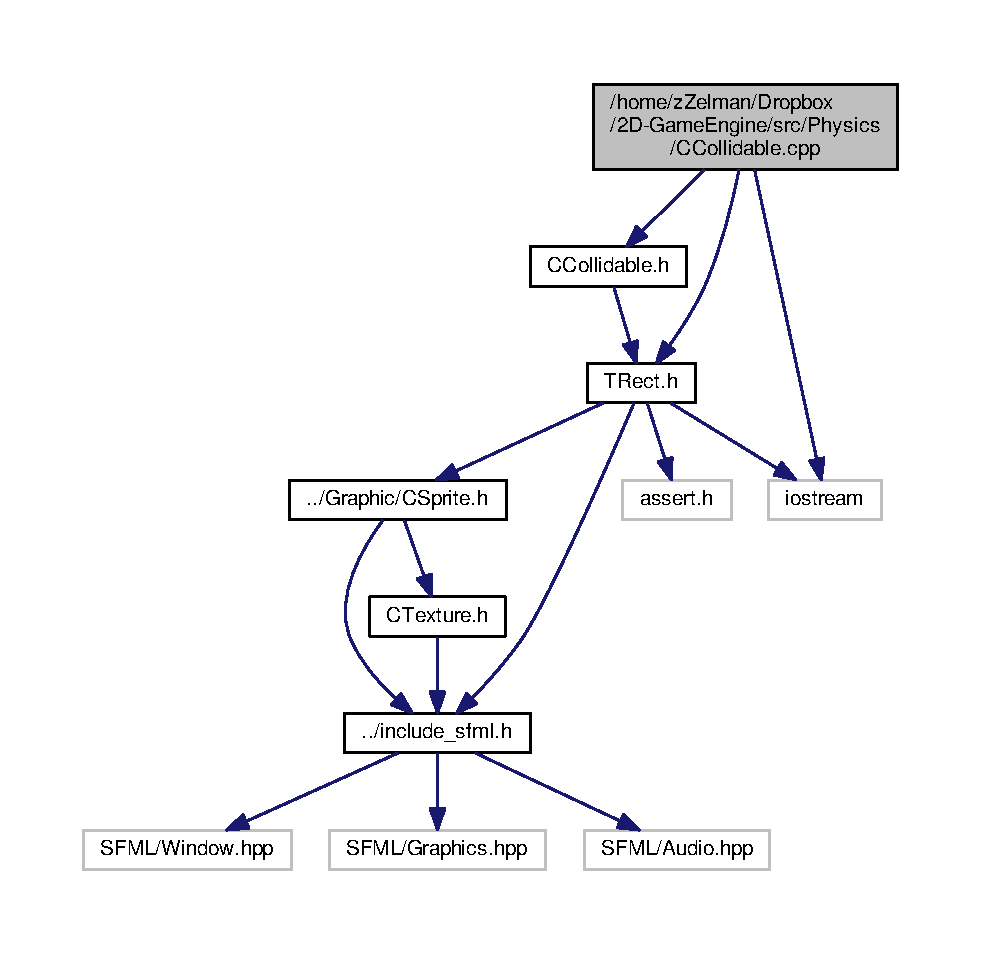
\includegraphics[width=350pt]{CCollidable_8cpp__incl}
\end{center}
\end{figure}
\subsection*{Namespaces}
\begin{DoxyCompactItemize}
\item 
\hyperlink{namespaceengine}{engine}
\end{DoxyCompactItemize}

\hypertarget{CCollidable_8h}{\section{/home/z\-Zelman/\-Dropbox/2\-D-\/\-Game\-Engine/src/\-Physics/\-C\-Collidable.h File Reference}
\label{CCollidable_8h}\index{/home/z\-Zelman/\-Dropbox/2\-D-\/\-Game\-Engine/src/\-Physics/\-C\-Collidable.\-h@{/home/z\-Zelman/\-Dropbox/2\-D-\/\-Game\-Engine/src/\-Physics/\-C\-Collidable.\-h}}
}
{\ttfamily \#include \char`\"{}T\-Rect.\-h\char`\"{}}\\*
Include dependency graph for C\-Collidable.\-h\-:
\nopagebreak
\begin{figure}[H]
\begin{center}
\leavevmode
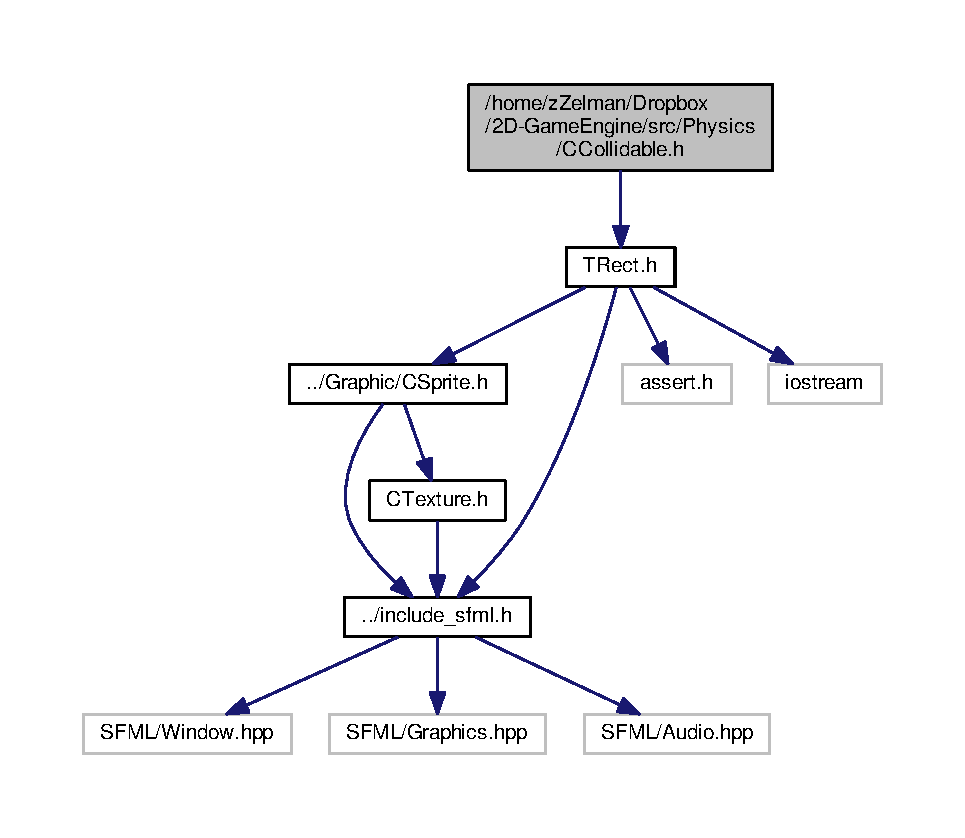
\includegraphics[width=350pt]{CCollidable_8h__incl}
\end{center}
\end{figure}
This graph shows which files directly or indirectly include this file\-:
\nopagebreak
\begin{figure}[H]
\begin{center}
\leavevmode
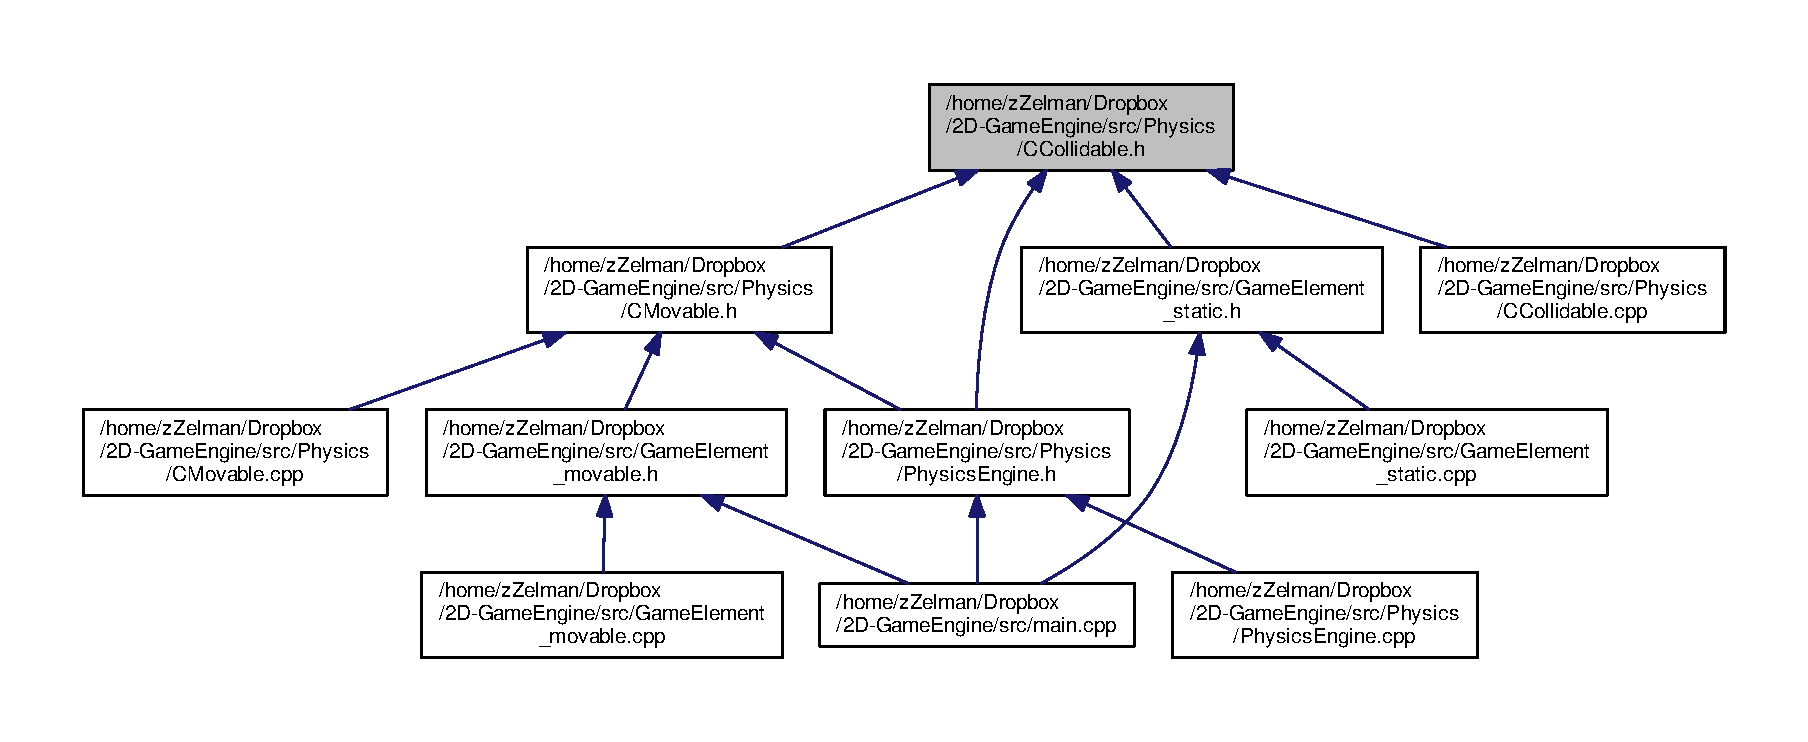
\includegraphics[width=350pt]{CCollidable_8h__dep__incl}
\end{center}
\end{figure}
\subsection*{Classes}
\begin{DoxyCompactItemize}
\item 
class \hyperlink{classengine_1_1CCollidable}{engine\-::\-C\-Collidable}
\begin{DoxyCompactList}\small\item\em The base class for all physics objects. \end{DoxyCompactList}\end{DoxyCompactItemize}
\subsection*{Namespaces}
\begin{DoxyCompactItemize}
\item 
\hyperlink{namespaceengine}{engine}
\end{DoxyCompactItemize}

\hypertarget{CMovable_8cpp}{\section{/home/z\-Zelman/\-Dropbox/2\-D-\/\-Game\-Engine/src/\-Physics/\-C\-Movable.cpp File Reference}
\label{CMovable_8cpp}\index{/home/z\-Zelman/\-Dropbox/2\-D-\/\-Game\-Engine/src/\-Physics/\-C\-Movable.\-cpp@{/home/z\-Zelman/\-Dropbox/2\-D-\/\-Game\-Engine/src/\-Physics/\-C\-Movable.\-cpp}}
}
{\ttfamily \#include \char`\"{}C\-Movable.\-h\char`\"{}}\\*
{\ttfamily \#include $<$iostream$>$}\\*
Include dependency graph for C\-Movable.\-cpp\-:\nopagebreak
\begin{figure}[H]
\begin{center}
\leavevmode
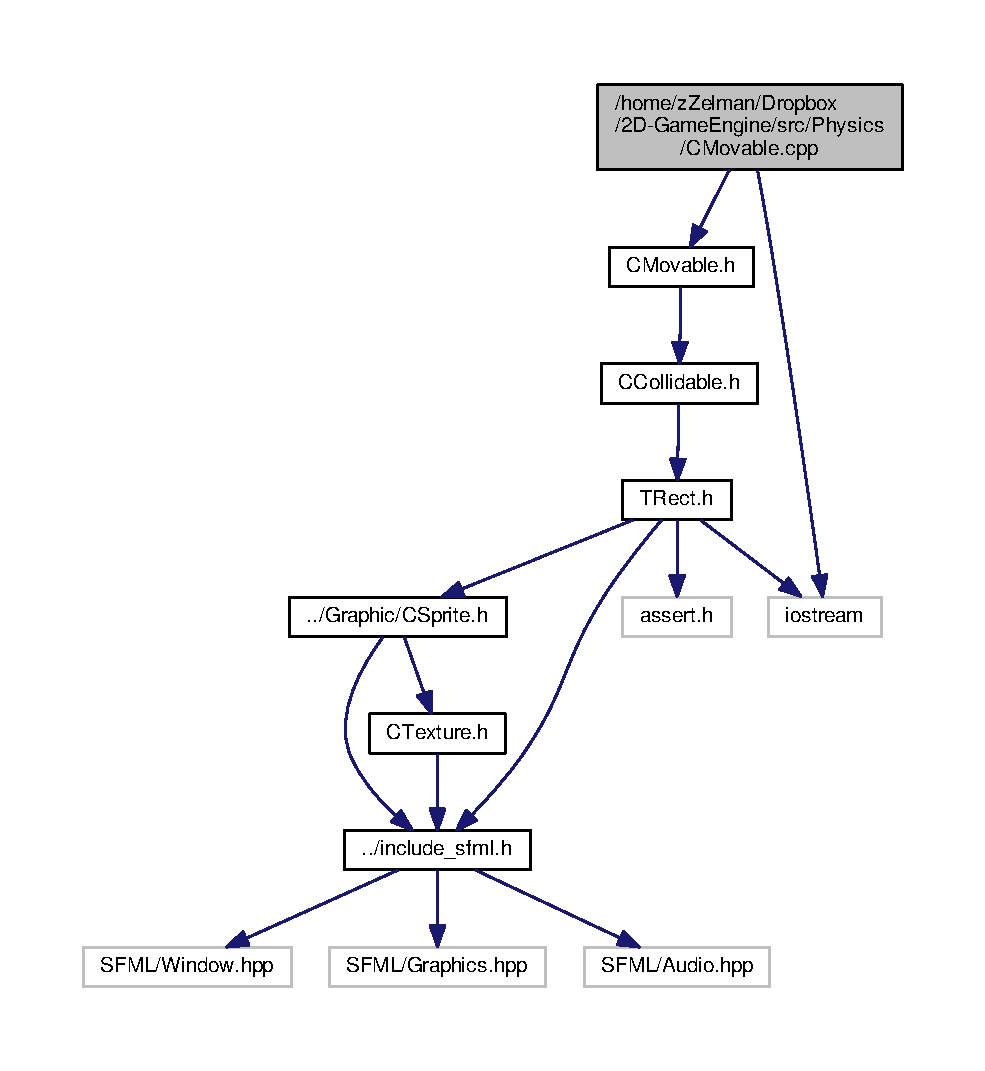
\includegraphics[width=350pt]{CMovable_8cpp__incl}
\end{center}
\end{figure}
\subsection*{Namespaces}
\begin{DoxyCompactItemize}
\item 
\hyperlink{namespaceengine}{engine}
\end{DoxyCompactItemize}

\hypertarget{CMovable_8h}{\section{/home/z\-Zelman/\-Dropbox/2\-D-\/\-Game\-Engine/src/\-Physics/\-C\-Movable.h File Reference}
\label{CMovable_8h}\index{/home/z\-Zelman/\-Dropbox/2\-D-\/\-Game\-Engine/src/\-Physics/\-C\-Movable.\-h@{/home/z\-Zelman/\-Dropbox/2\-D-\/\-Game\-Engine/src/\-Physics/\-C\-Movable.\-h}}
}
{\ttfamily \#include \char`\"{}C\-Collidable.\-h\char`\"{}}\\*
Include dependency graph for C\-Movable.\-h\-:\nopagebreak
\begin{figure}[H]
\begin{center}
\leavevmode
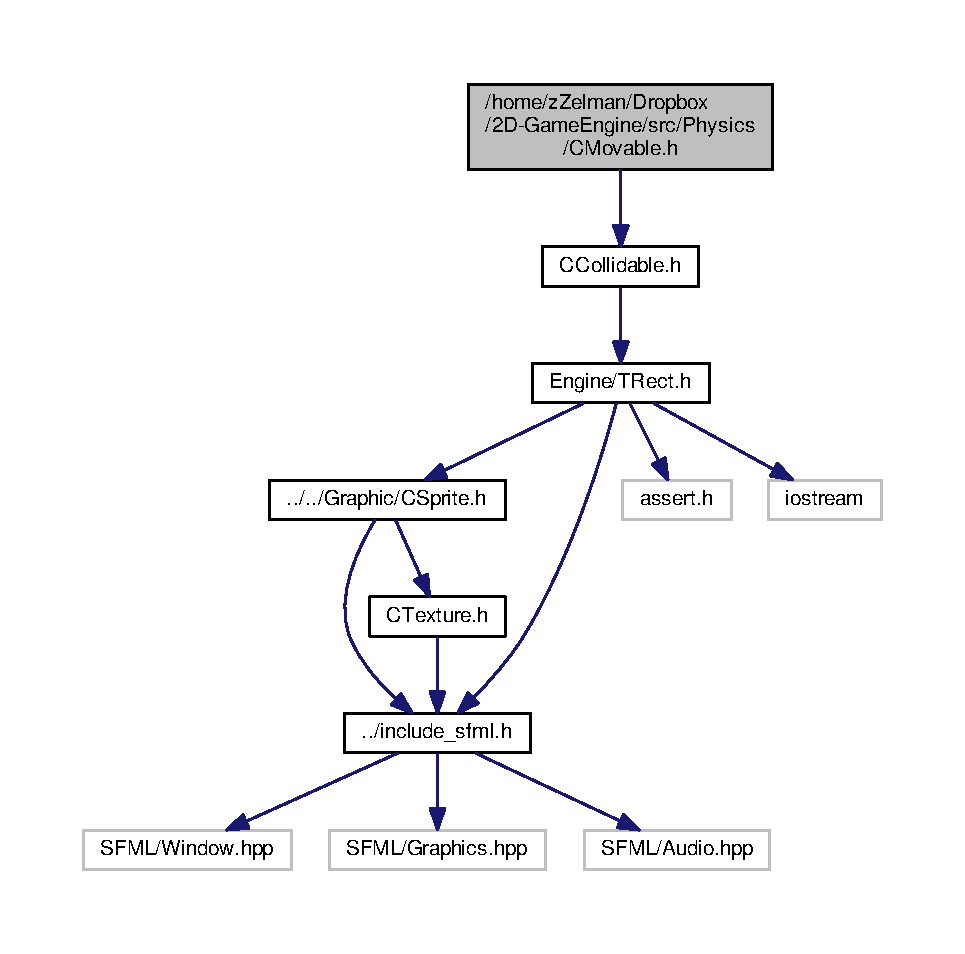
\includegraphics[width=350pt]{CMovable_8h__incl}
\end{center}
\end{figure}
This graph shows which files directly or indirectly include this file\-:\nopagebreak
\begin{figure}[H]
\begin{center}
\leavevmode
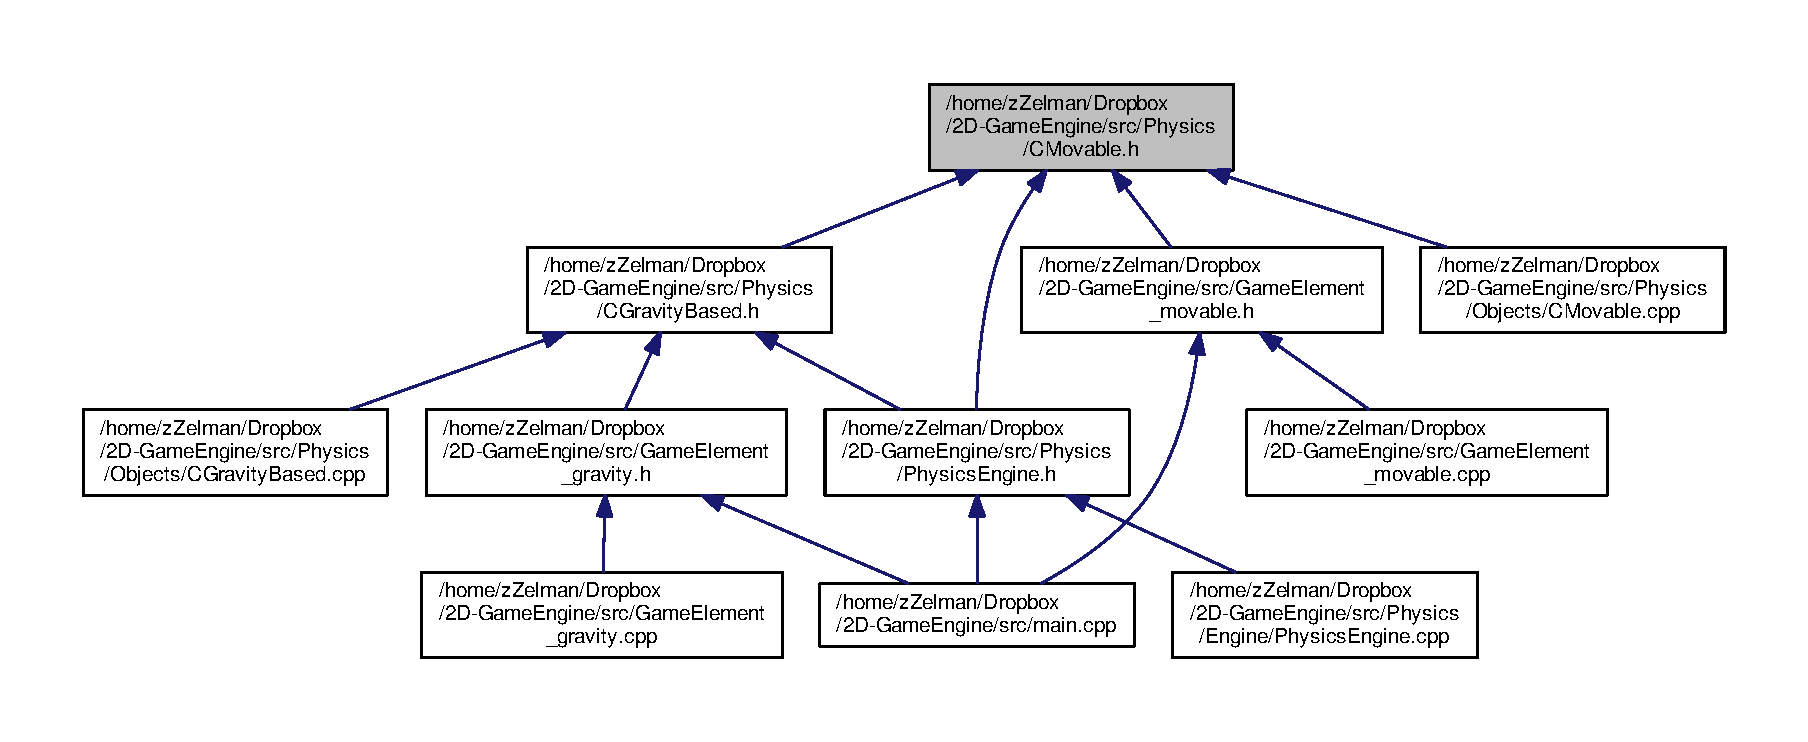
\includegraphics[width=350pt]{CMovable_8h__dep__incl}
\end{center}
\end{figure}
\subsection*{Classes}
\begin{DoxyCompactItemize}
\item 
struct \hyperlink{structengine_1_1SSideBlocked}{engine\-::\-S\-Side\-Blocked}
\begin{DoxyCompactList}\small\item\em A plane-\/old-\/data-\/structure to tell whether the directions are \char`\"{}physically\char`\"{} blocked for movement. \end{DoxyCompactList}\item 
class \hyperlink{classengine_1_1CMovable}{engine\-::\-C\-Movable}
\end{DoxyCompactItemize}
\subsection*{Namespaces}
\begin{DoxyCompactItemize}
\item 
\hyperlink{namespaceengine}{engine}
\end{DoxyCompactItemize}

\hypertarget{PhysicsEngine_8cpp}{\section{/home/z\-Zelman/\-Dropbox/2\-D-\/\-Game\-Engine/src/\-Physics/\-Engine/\-Physics\-Engine.cpp File Reference}
\label{PhysicsEngine_8cpp}\index{/home/z\-Zelman/\-Dropbox/2\-D-\/\-Game\-Engine/src/\-Physics/\-Engine/\-Physics\-Engine.\-cpp@{/home/z\-Zelman/\-Dropbox/2\-D-\/\-Game\-Engine/src/\-Physics/\-Engine/\-Physics\-Engine.\-cpp}}
}
{\ttfamily \#include \char`\"{}../\-Physics\-Engine.\-h\char`\"{}}\\*
{\ttfamily \#include $<$iostream$>$}\\*
Include dependency graph for Physics\-Engine.\-cpp\-:\nopagebreak
\begin{figure}[H]
\begin{center}
\leavevmode
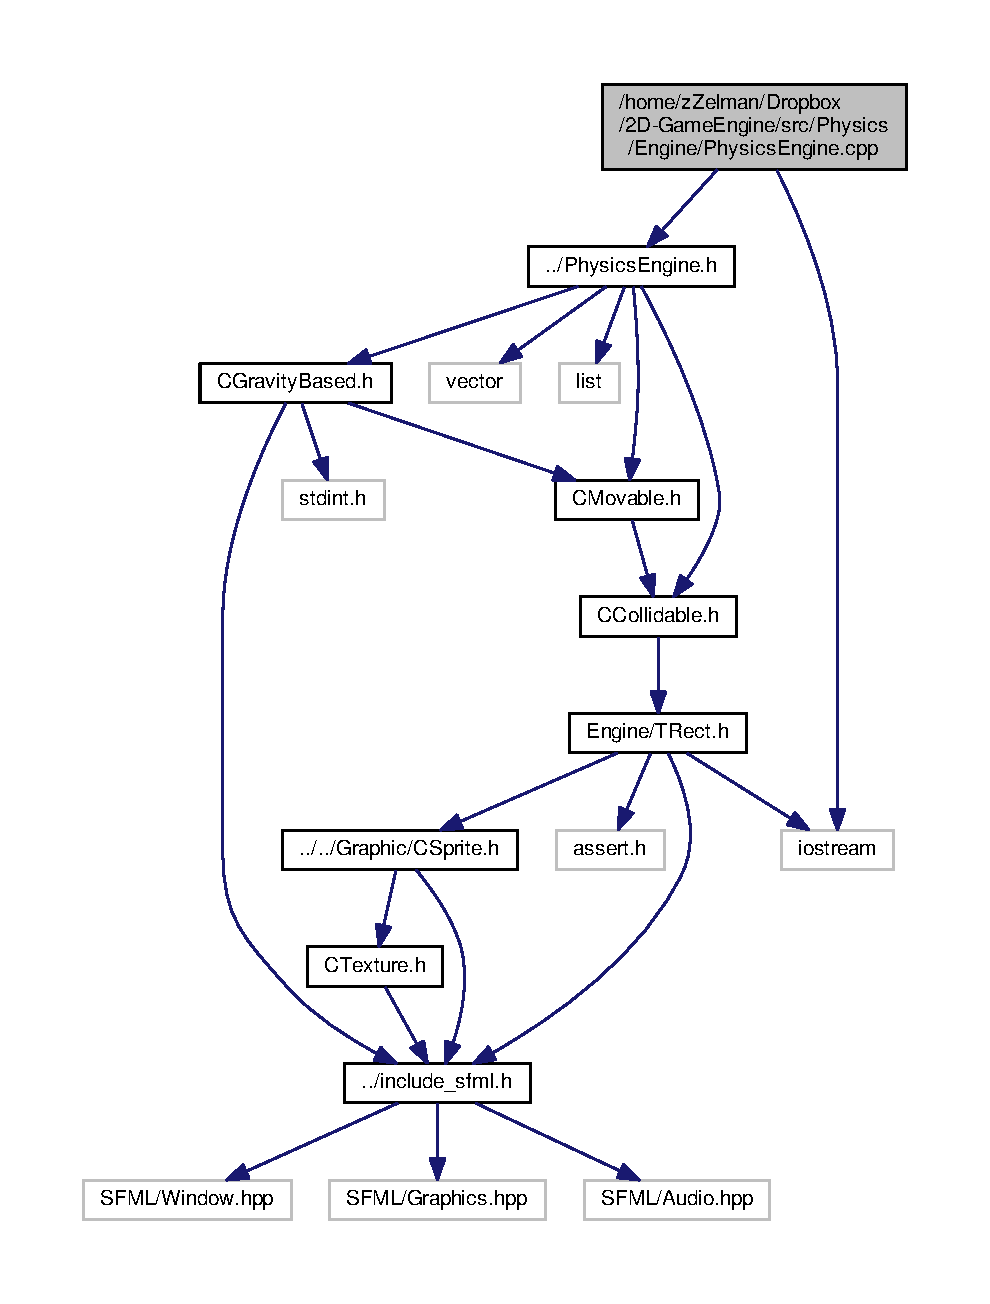
\includegraphics[width=350pt]{PhysicsEngine_8cpp__incl}
\end{center}
\end{figure}
\subsection*{Namespaces}
\begin{DoxyCompactItemize}
\item 
\hyperlink{namespaceengine}{engine}
\end{DoxyCompactItemize}

\hypertarget{PhysicsEngine_8h}{\section{/home/z\-Zelman/\-Dropbox/2\-D-\/\-Game\-Engine/src/\-Physics/\-Physics\-Engine.h File Reference}
\label{PhysicsEngine_8h}\index{/home/z\-Zelman/\-Dropbox/2\-D-\/\-Game\-Engine/src/\-Physics/\-Physics\-Engine.\-h@{/home/z\-Zelman/\-Dropbox/2\-D-\/\-Game\-Engine/src/\-Physics/\-Physics\-Engine.\-h}}
}
{\ttfamily \#include \char`\"{}C\-Collidable.\-h\char`\"{}}\\*
{\ttfamily \#include \char`\"{}C\-Movable.\-h\char`\"{}}\\*
{\ttfamily \#include $<$vector$>$}\\*
{\ttfamily \#include $<$list$>$}\\*
Include dependency graph for Physics\-Engine.\-h\-:
\nopagebreak
\begin{figure}[H]
\begin{center}
\leavevmode
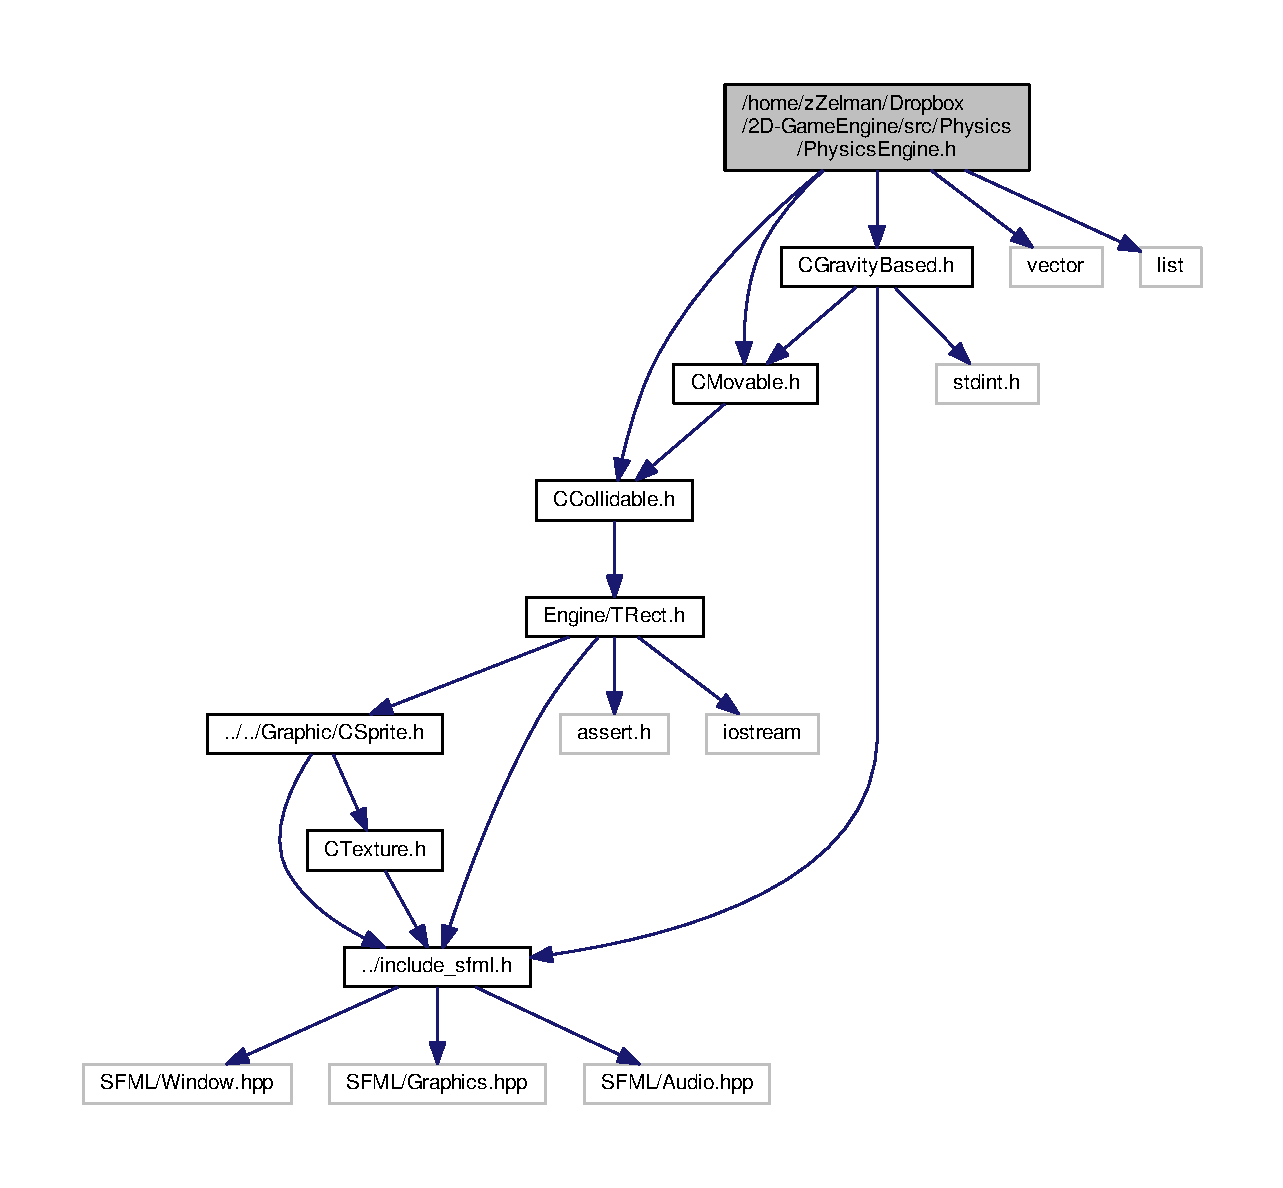
\includegraphics[width=350pt]{PhysicsEngine_8h__incl}
\end{center}
\end{figure}
This graph shows which files directly or indirectly include this file\-:\nopagebreak
\begin{figure}[H]
\begin{center}
\leavevmode
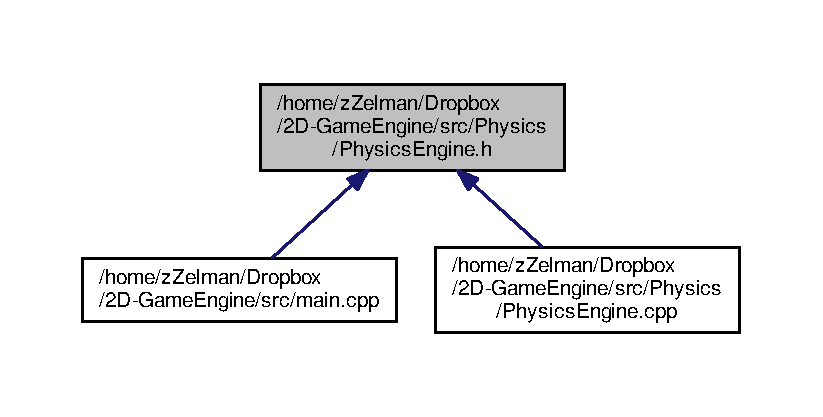
\includegraphics[width=350pt]{PhysicsEngine_8h__dep__incl}
\end{center}
\end{figure}
\subsection*{Classes}
\begin{DoxyCompactItemize}
\item 
class \hyperlink{classengine_1_1PhysicsEngine}{engine\-::\-Physics\-Engine}
\end{DoxyCompactItemize}
\subsection*{Namespaces}
\begin{DoxyCompactItemize}
\item 
\hyperlink{namespaceengine}{engine}
\end{DoxyCompactItemize}

\hypertarget{TRect_8h}{\section{/home/z\-Zelman/\-Dropbox/2\-D-\/\-Game\-Engine/src/\-Physics/\-Engine/\-T\-Rect.h File Reference}
\label{TRect_8h}\index{/home/z\-Zelman/\-Dropbox/2\-D-\/\-Game\-Engine/src/\-Physics/\-Engine/\-T\-Rect.\-h@{/home/z\-Zelman/\-Dropbox/2\-D-\/\-Game\-Engine/src/\-Physics/\-Engine/\-T\-Rect.\-h}}
}
{\ttfamily \#include \char`\"{}../../\-Graphic/\-C\-Sprite.\-h\char`\"{}}\\*
{\ttfamily \#include \char`\"{}../../include\-\_\-sfml.\-h\char`\"{}}\\*
{\ttfamily \#include $<$assert.\-h$>$}\\*
{\ttfamily \#include $<$iostream$>$}\\*
Include dependency graph for T\-Rect.\-h\-:\nopagebreak
\begin{figure}[H]
\begin{center}
\leavevmode
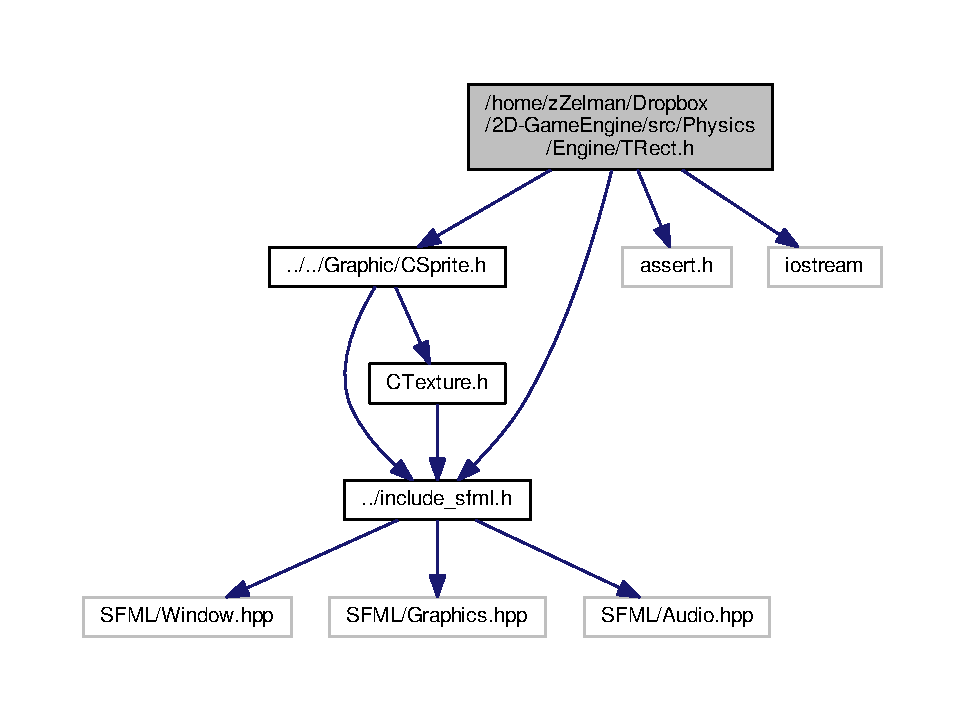
\includegraphics[width=350pt]{TRect_8h__incl}
\end{center}
\end{figure}
This graph shows which files directly or indirectly include this file\-:\nopagebreak
\begin{figure}[H]
\begin{center}
\leavevmode
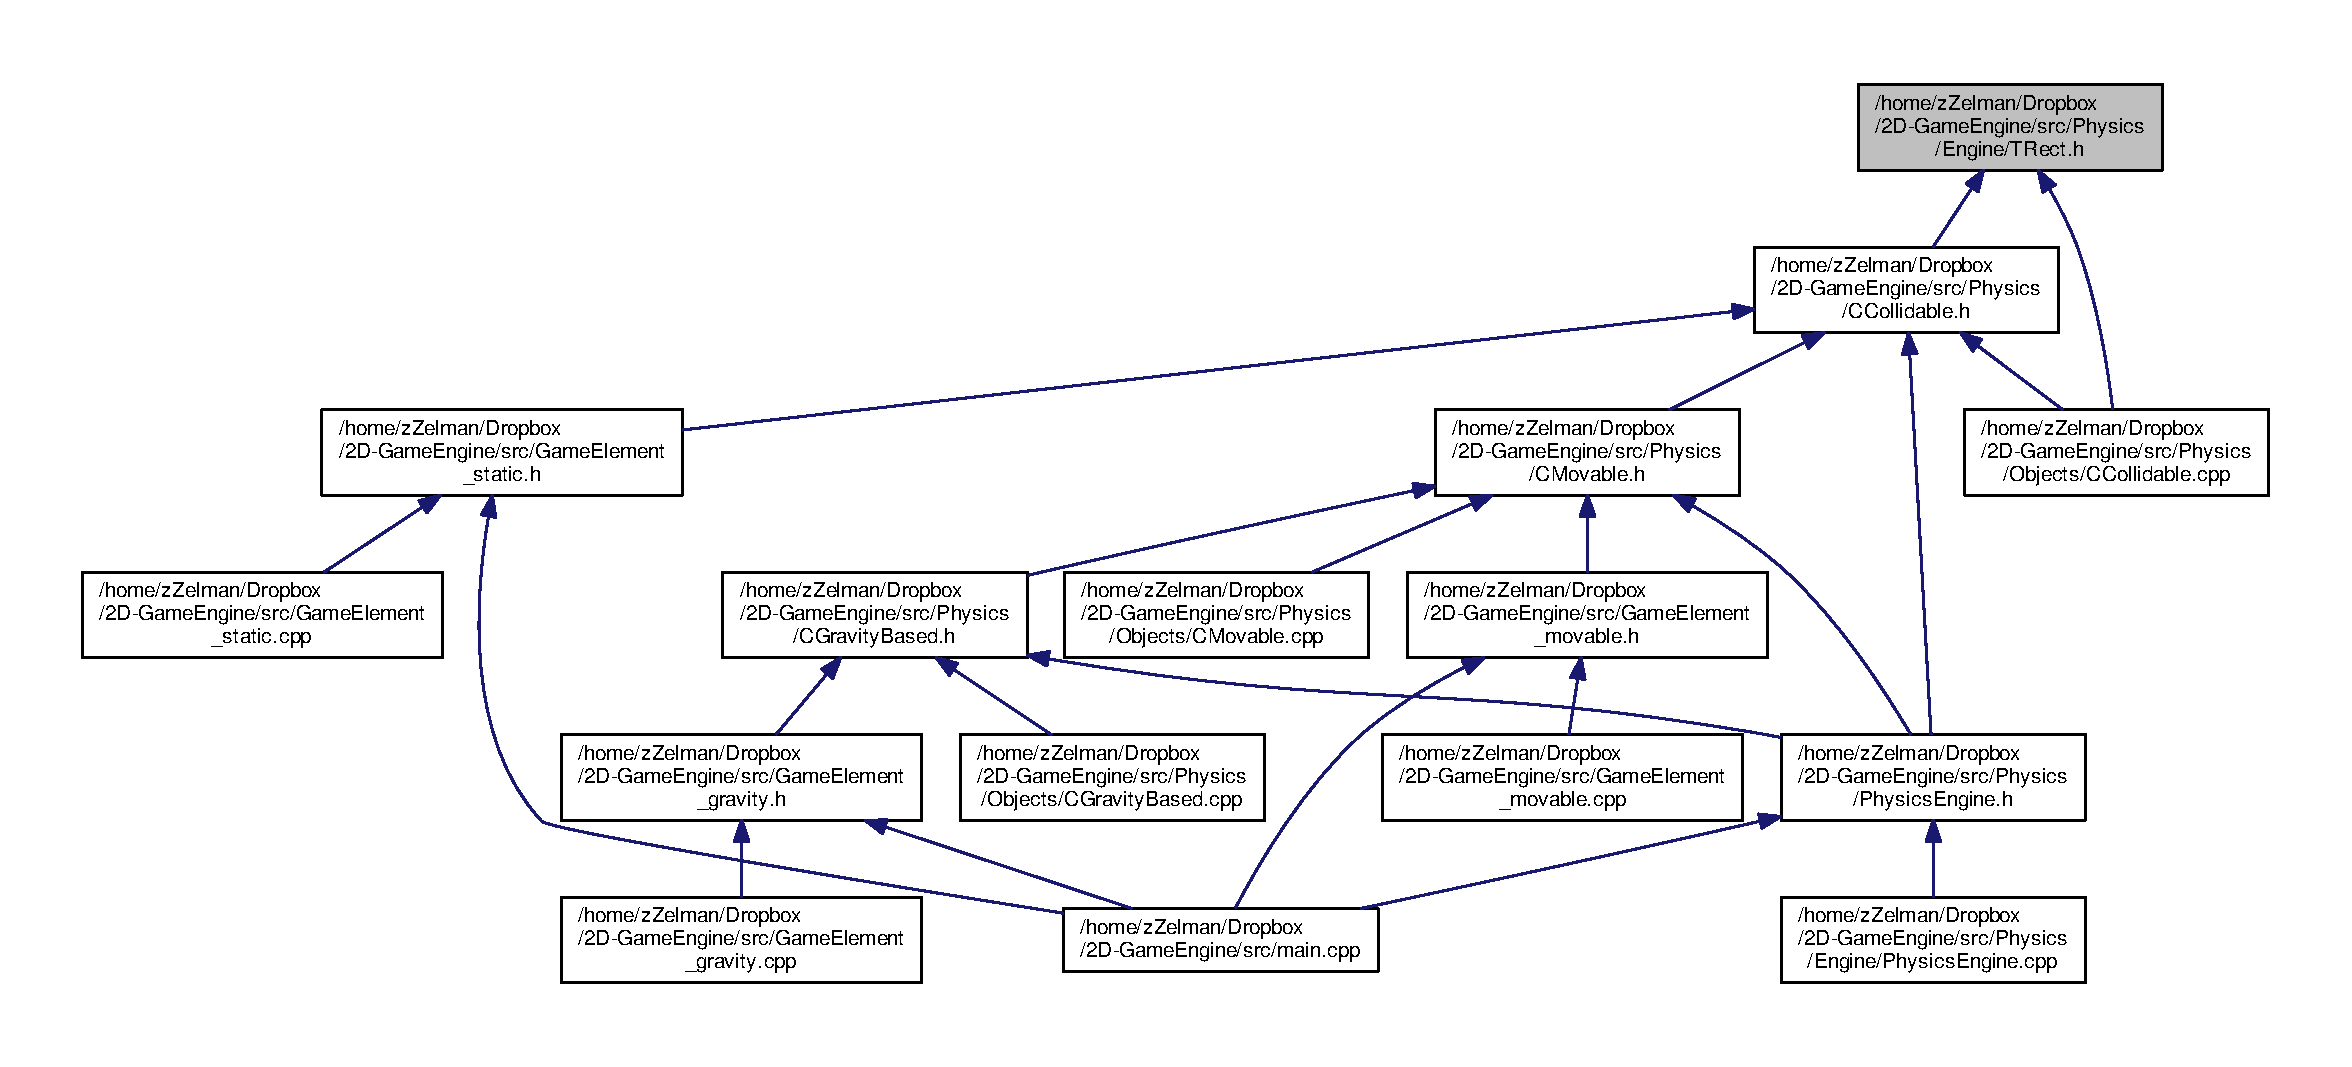
\includegraphics[width=350pt]{TRect_8h__dep__incl}
\end{center}
\end{figure}
\subsection*{Classes}
\begin{DoxyCompactItemize}
\item 
class \hyperlink{classengine_1_1TRect}{engine\-::\-T\-Rect$<$ T $>$}
\begin{DoxyCompactList}\small\item\em A template class for a Rectangle that the physics engine uses. \end{DoxyCompactList}\end{DoxyCompactItemize}
\subsection*{Namespaces}
\begin{DoxyCompactItemize}
\item 
\hyperlink{namespaceengine}{engine}
\end{DoxyCompactItemize}

%--- End generated contents ---

% Index
\newpage
\phantomsection
\addcontentsline{toc}{part}{Index}
\printindex

\end{document}
